%  --------------------------------------------------------------------------
%  Diplomarbeit Dokumentation
%  Created by Silvan Spross on 2011-04-02.
%  --------------------------------------------------------------------------

%  --------------------------------------------------------------------------
%  Latex Document Settings
%  --------------------------------------------------------------------------
\documentclass[
11pt, % Schriftgrösse
a4paper, % A4 Papier
BCOR10mm, % Absoluter Wert der Bindekorrektur, z.B. BCOR1cm
DIV14, % Satzspiegel festlegen siehe
       % http://www.ctex.org/documents/packages/nonstd/koma-script.pdf
footsepline = false, % Trennlinie zwischen Textkörper und Fußzeile
                     % bei normalen Seiten
headsepline, % Trennlinie zwischen Kopfzeile und Textkörper
             % bei normalen Seiten
oneside, % Zweiseitig
openright,
halfparskip, % Europäischer Satz mit Abstand zwischen den Absätzen
abstracton, % inkl. Abstract
listof=totocnumbered, % Abb.- und Tab.verzeichnis im Inhaltsverzeichnis
bibliography=totocnumbered % Lit.zeichnis in Inhaltsverzeichnis aufnehmen
]{scrreprt}

\usepackage[automark]{scrpage2} % Gestaltung von kopf- und Fußzeile
\usepackage[ngerman]{babel}
\usepackage[ngerman]{translator}
\usepackage{tocbasic}
\usepackage[utf8]{inputenc}
\usepackage{lmodern} % Latin Modern
\usepackage[T1]{fontenc}
\usepackage{hyphenat}
\usepackage{ae} % Schöne Schriften für PDF-Dateien

% Tradmark
\def\TTra{\textsuperscript{\texttrademark}}

%1.5 Zeilenabstand
\usepackage[onehalfspacing]{setspace}

% Festlegung des Seitenstils (scrpage2)
\pagestyle{scrheadings}
\clearscrheadfoot
\automark[chapter]{section}

% \lehead{\sffamily\upshape\headmark}
% \cehead{}
% \rehead{}
% \lefoot[\pagemark]{\upshape \pagemark}
% \cefoot{}
% \refoot{}
% \lohead{}
% \cohead{}
\lohead{\sffamily\upshape\headmark}
\lofoot{}
\cofoot{}
\rofoot[\pagemark]{\scshape \pagemark}

% Surround parts of graphics with box
\usepackage{boxedminipage}

% Package for including code in the document
\usepackage{listings}

% If you want to generate a toc for each chapter (use with book)
\usepackage{minitoc}
\usepackage{longtable}

% Abkürzungsverzeichnis erstellen.
\usepackage[printonlyused]{acronym}

% schöne Tabelle zeichnen
\usepackage{booktabs}
\renewcommand{\arraystretch}{1.4} %Die Zeilenabstände in Tabllen angepasst.

% für variable Breiten
\usepackage{tabularx}

% Durchgestrichener Text
\usepackage[normalem]{ulem} %emphasize weiterhin kursiv

% This is now the recommended way for checking for PDFLaTeX:
\usepackage{ifpdf}

\usepackage{eurosym}

\usepackage{natbib}

\usepackage{paralist}

\usepackage[hyperfootnotes=false]{hyperref}
\hypersetup{
  bookmarks=true,         % show bookmarks bar?
  unicode=true,           % non-Latin characters in Acrobat’s bookmarks
  pdftoolbar=true,        % show Acrobat’s toolbar?
  pdfmenubar=true,        % show Acrobat’s menu?
  pdffitwindow=true,      % window fit to page when opened
  pdfstartview={FitH},    % fits the width of the page to the window
  pdftitle={Diplomarbeit},   
  pdfauthor={Silvan Spross},
  pdfsubject={Definition und Optimierung der Projektprozesse bei allink.creative},
  pdfcreator={TeX Live 2009},
  pdfproducer={pdfTeX, Version 3.1415926-1.40.10},
  pdfnewwindow=true,      % links in new window
  colorlinks=true,       % false: boxed links; true: colored links
  linkcolor=blue,          % color of internal links
  citecolor=black,        % color of links to bibliography
  filecolor=magenta,      % color of file links
  urlcolor=cyan          % color of external links
  % linkcolor=black,          % color of internal links
  % citecolor=black,        % color of links to bibliography
  % filecolor=black,      % color of file links
  % urlcolor=black          % color of external links
}

\ifpdf
    \usepackage[pdftex]{graphicx}
\else
    \usepackage{graphicx}
\fi

\makeatletter 
\let\orgdescriptionlabel\descriptionlabel 
\renewcommand*{\descriptionlabel}[1]{% 
  \let\orglabel\label 
  \let\label\@gobble 
  \phantomsection 
  \edef\@currentlabel{#1}% 
  %\edef\@currentlabelname{#1}% 
  \let\label\orglabel 
  \orgdescriptionlabel{#1}% 
} 
\makeatother 

%  --------------------------------------------------------------------------
%  Start Document
%  --------------------------------------------------------------------------
\title{Definition und Optimierung der Projektprozesse bei allink.creative}

\author{Diplomarbeit in Informatik\\
    \\
    Studierender - Silvan Spross\\
	Auftraggeber - Michael Walder\\
    Projektbetreuer - Beat Seeliger\\
    Experte - Matthias Bachmann\\
	\\
	HSZ-T - Technische Hochschule Zürich}

\date{März 2011 bis Juni 2011}

\begin{document}

  \ifpdf
    \DeclareGraphicsExtensions{.pdf, .jpg, .tif}
  \else
    \DeclareGraphicsExtensions{.eps, .jpg}
  \fi

  \pagenumbering{Alph}
  
  \maketitle

  \begin{abstract}
Die Designagentur allink.creative stellt sich wegen ihres Wachstums neuen 
Herausforderungen in ihren Projektabläufen und Prozessen. Da sich die
Agentur bis anhin noch nicht mit diesem Thema explizit auseinander gesetzt hat,
wird im Rahmen dieser Arbeit der heutigen Zustand genauer analysiert und 
zusammen mit den Bedürfnissen und Anforderungen erfasst. Zusätzlich wird ein
Branchenvergleich zwischen ähnlichen Agenturen durchgeführt.
Anhand den gewonnenen Informationen und den vorhandenen Theorien wird ein Konzept
mit praxisnahen Lösungsvarianten aufgezeigt. Die gewählte
Variante wird in einem ``Proof of Concept'' getestet und aus den daraus
entstehenden Resultaten werden Schlüsse für die zukünftige Vorgehensweise 
gezogen. Über die ganze Arbeit hinweg stehen auch die zur Zeit und in Zukunft zu verwendenden
Tools und Software zur Unterstützung im Vordergrund.
\end{abstract}

  \pagenumbering{Roman}
  
  \tableofcontents
  
  \chapter{Personalienblatt}
  \begin{tabbing}
	\hspace*{4cm}   \= \kill
	Name, Vorname:  \> {\bf Spross, Silvan} \\
	Adresse:        \> {\bf Meinrad Lienert-Strasse 27} \\
	PLZ, Wohnort:   \> {\bf 8003 Zürich} \\
	\\
	Geburtsdatum:   \> {\bf 07.11.1985} \\
	Heimatort:      \> {\bf Zürich ZH} \\
\end{tabbing}

  
  \chapter{Bestätigung}
  Hiermit bestätige ich, Silvan Spross, dass die vorliegende Diplomarbeit 
``Definition und Optimierung der Projektprozesse bei allink.creative'' im
Rahmen der geltenden Reglemente und in allen Teilen selbständig erarbeitet und 
durchgeführt wurde.\\
\\
Zürich, den 31. Mai 2011\\
\\\\
Silvan Spross
  
  \chapter{Vorwort}
  Das Schreiben einer Diplomarbeit bedeutet nebst dem baldigen Abschluss des Studiums
auch einen grossen Aufwand. Deshalb ist die Wahl des Themas und meine
Motivation in diese Arbeit die nötige Zeit und Qualität zu investieren sehr
wichtig. Aus diesem Grund möchte ich kurz erläutern, was mich zu dieser
Arbeit geführt hat.

Ein eigenes Unternehmen zu gründen und erfolgreich zu führen war schon immer
einer meiner Träume. Nach meiner Lehre im Jahre 2004 machte ich mich deshalb
selbstständig und gründete 2005 die SiSprocom GmbH\footnote{Website der SiSprocom GmbH, \url{http://sisprocom.ch/}}. 
Im ersten Jahr bestanden
die Tätigkeitsfelder überwiegend aus Webdesign und Schulungen. Im Bereich
Webdesign lag der Fokus hauptsächlich auf der Programmierung. Dieser Bereich 
entwickelte sich immer stärker in Richtung 
Applikationsentwicklung und dank Aufträgen einer Zürcher Grossbank 
lag der Fokus bald nur noch darauf.

Durch dieses grössere Mandat wuchs die SiSprocom GmbH zwischenzeitlich
auf 3 Mitarbeiter. Dies führte zu massiv mehr Aufwand in der Administration.
Schnell wurde klar, dass zwingend Stunden rapportiert und das Schreiben
von Rechnungen vereinfacht werden musste. Wir bedienten uns damals Google 
Docs\footnote{Googles Online Office Suite, \url{http://docs.google.com/}} um die rapportierten Stunden zentral zu 
verwalten und einer selbst geschriebenen Software um vereinfacht Rechnungen 
verwalten und schreiben zu können.
So lehrreich und spannend die Arbeit in dieser Grossbank auch war, so kompliziert
waren auch ihre Abläufe und Prozesse. Zu diesem Zeitpunkt schwor ich mir, dies
in meiner Unternehmung einmal besser zu lösen.

Ende 2009 realisierte ich, dass ich zwar ein eigenes Unternehmen hatte und
selbständig war, jedoch fast ausschliesslich nur für einen Kunden arbeitete.
Ich kam zum Schluss, dass dies nicht das eigentliches Ziel meiner Selbständigkeit 
war und begriff
relativ schnell, dass ich mich von dieser Abhängigkeit nur lösen konnte, wenn
ich mich als Person vollständig aus diesem Mandat zurückziehe.
Dies tat ich dann anfangs 2010 auch und mietete ein Büro in den Räumlichkeiten
der allink GmbH\footnote{Website der allink GmbH, \url{http://allink.ch/}}. Deren IT hatte zu diesem Zeitpunkt 
ein paar grössere
Herausforderungen zu bewältigen und ich bot meine Hilfe an. Schnell wurde
daraus eine Partnerschaft und die SiSprocom fusionierte mit der allink, indem zwischen
den Partnern Anteile der jeweiligen Firma ausgetauscht wurden.

Heute, im März 2011, knapp ein Jahr danach, ist Die SiSprocom GmbH um 30\% 
gewachsen und arbeitet ausschliesslich für die erwähnte Grossbank. Alle anderen Projekte
haben wir in die allink GmbH übernommen. Die administrativen Aufgaben der
SiSprocom GmbH wurden an
meinem Vater abgetreten, der zusammen mit einem Treuhänder das laufende
Mandat und die drei Mitarbeiter gut handhaben kann. So konnte ich mich ganz
auf die neuen Herausforderungen bei der allink konzentrieren.

Die allink GmbH ist inzwischen um 70\% auf 17 Mitarbeiter gewachsen und muss sich dadurch
neuen Herausforderungen in der Organisation und bei den Projektabläufen stellen.

Da mich die Selbständigkeit auch durch das ganze Studium begleitet hat, möchte 
ich meine Diplomarbeit nutzen um unser Unternehmen zu optimieren.
  
  \chapter{Einleitung}
  \pagenumbering{arabic}
  \section{Ausgangslage}
Die Agentur allink.creative ist im letzten Jahr stark gewachsen. Von zehn
Mitarbeitern im Februar 2010 auf siebzehn Mitarbeiter im Februar 2011. Dies hat 
zur Auswirkung, dass gewisse Abläufe und Prozesse neu definiert und bestehende
überarbeitet werden müssen, um weiterhin effizient, oder wenn möglich noch 
effizienter, arbeiten zu können. Die Agentur arbeitet zurzeit überwiegend mit Apple
Computern und setzt gewisse Software ein, die die Geschäftsleitung beibehalten 
möchte. Es soll jedoch innerhalb dieser Arbeit geprüft werden, welche Software
weiterhin Sinn macht und welche man möglicherweise ersetzen oder neu anschaffen
bzw. sogar selbst entwickeln möchte.

\section{Problemstellung}
Durch den schnellen Wachstum der Agentur stösst sie bei der Abwicklung ihrer
Projekte an Grenzen. Die Partner, die bisher den Überblick über alle
Projekte und deren Abläufe im Auge behalten konnten, sind bei dieser Grösse
nicht mehr in der Lage dies beizubehalten. Deshalb muss mehr Struktur geschaffen und
den Mitarbeitern mehr Verantwortung und Kompetenzen abgegeben werden. Und trotzdem
soll es der Geschäftsleitung mit Hilfe von Controling Tools möglich bleiben,
einen Überblick über die Lage der Agentur zu behalten.

Die Partner erhoffen sich dadurch ein gesundes Wachstum der Agentur ermöglichen
zu können. Zusätzlich wird vermutet, dass durch Optimierungen im Projektablauf
auch Kosten gespart werden können und die ganze Agentur im Allgemeinen 
professionalisiert werden kann.

\section{Zielsetzung}
Das Hauptziel dieser Arbeit besteht darin, das aktuelle Projektmanagement der 
allink zu analysieren, den zur Zeit gegebenen Umständen anzupassen und zu
optimieren, damit ein weiteres Wachstum der Agentur vereinfacht wird.

Allen Partnern bei der allink ist klar, dass der heutiger Projektablauf 
nicht optimal ist. Zu oft sehen sie sich mit gleichen Problemen konfrontiert, 
die in anderen Projekt schon einmal angetroffen und gelöst wurden.
Jedes Mal wird versucht daraus zu lernen, ohne etwas konkret festzuhalten oder
wirklich zu verändern. Das liegt meist daran, dass zu viel ansteht und
die internen Verbesserungen hinter die Aufträge und Wünsche der Kunden
gestellt werden.

Der aktuellen Projektablauf der allink wird genauer untersucht und auf 
dessen Stärken und Schwächen eingegangen. Danach werden die Bedürfnisse und 
Anforderungen der verschiedenen Stakeholdern des Projektablaufes aufgenommen und
Kennzahlen definiert, die in Zukunft bei einem verbesserten Projektablauf gemessen 
werden sollen. Daraus wird ein neues Konzept des überarbeiteten Projektablaufes 
mit verschiedenen Varianten in der Umsetzung erstellt und zusammen mit der 
Geschäftsleitung der allink entschieden, welchen Projektablauf 
man in Zukunft einsetzen und verfeinern möchte. Der neue Projektablauf soll 
abschliessend in einem ``Proof of Concept'', also anhand eines konkreten Projektes, 
getestet werden.

\section{Aufbau der Arbeit}
Im Kapitel \ref{chap:theorie_teil} werden dem Leser die Grundlagen zu Projektmanagement 
näher gebracht. Neben den jeweiligen Begriffserklärungen werden wichtige Modelle 
und Tools aus der Theorie und Praxis aufgezeigt.
Im Kapitel \ref{chap:analyse} wird der aktuelle Projektablauf bei der allink
GmbH genauer analysiert und aufgezeigt. Mit Hilfe der Prozessdarstellung wird
das aktuelle Vorgehen dargestellt und mit Beispielen untermalt.

Im Branchenvergleich im Kapitel \ref{chap:branchenvergleich} werden ähnlich 
grosse Agentur interviewt und deren Vorgehen als Vergleich herangezogen.
Im Kapitel \ref{chap:anforderungen} werden die Bedürfnisse und Anforderungen 
aller Stakeholders die in den Projektablauf involviert sind aufgenommen und daraus
Anforderungen gebildet. Zusätzlich werden Kennzahlen definiert, die in Zukunft
während und nach den Projekten gemessen werden sollen.

Im Kapitel \ref{chap:konzept} wird ein Lösungsansatz des neuen Projektablaufes
erarbeitet und verschiedene Varianten zur Umsetzung aufgezeigt. Auf dieser Grundlage
entscheidet sich der Auftraggeber für einen neuen Projektablauf. Dieser wird
im Kapitel \ref{chap:proof_of_concept} der Arbeit in einem ``Proof of Concept'' 
getestet. Im letzten Kapitel \ref{chap:reflektion} wird die Arbeit in Form eines Fazits 
zusammengefasst. Zudem wird ein Ausblick auf die zukünftige Verwendung und den 
Einsatz des neuen Projektablaufes abgegeben.

Die folgende Abbildung \ref{pic:01_gliederung_arbeit} beschreibt die Gliederung der 
Arbeit in graphischer Form und zeigt auf, wie die erarbeiteten Resultate in
den Lösungsansatz des neuen Projektablaufes einfliessen.

\begin{figure}[htbp]
\begin{center}
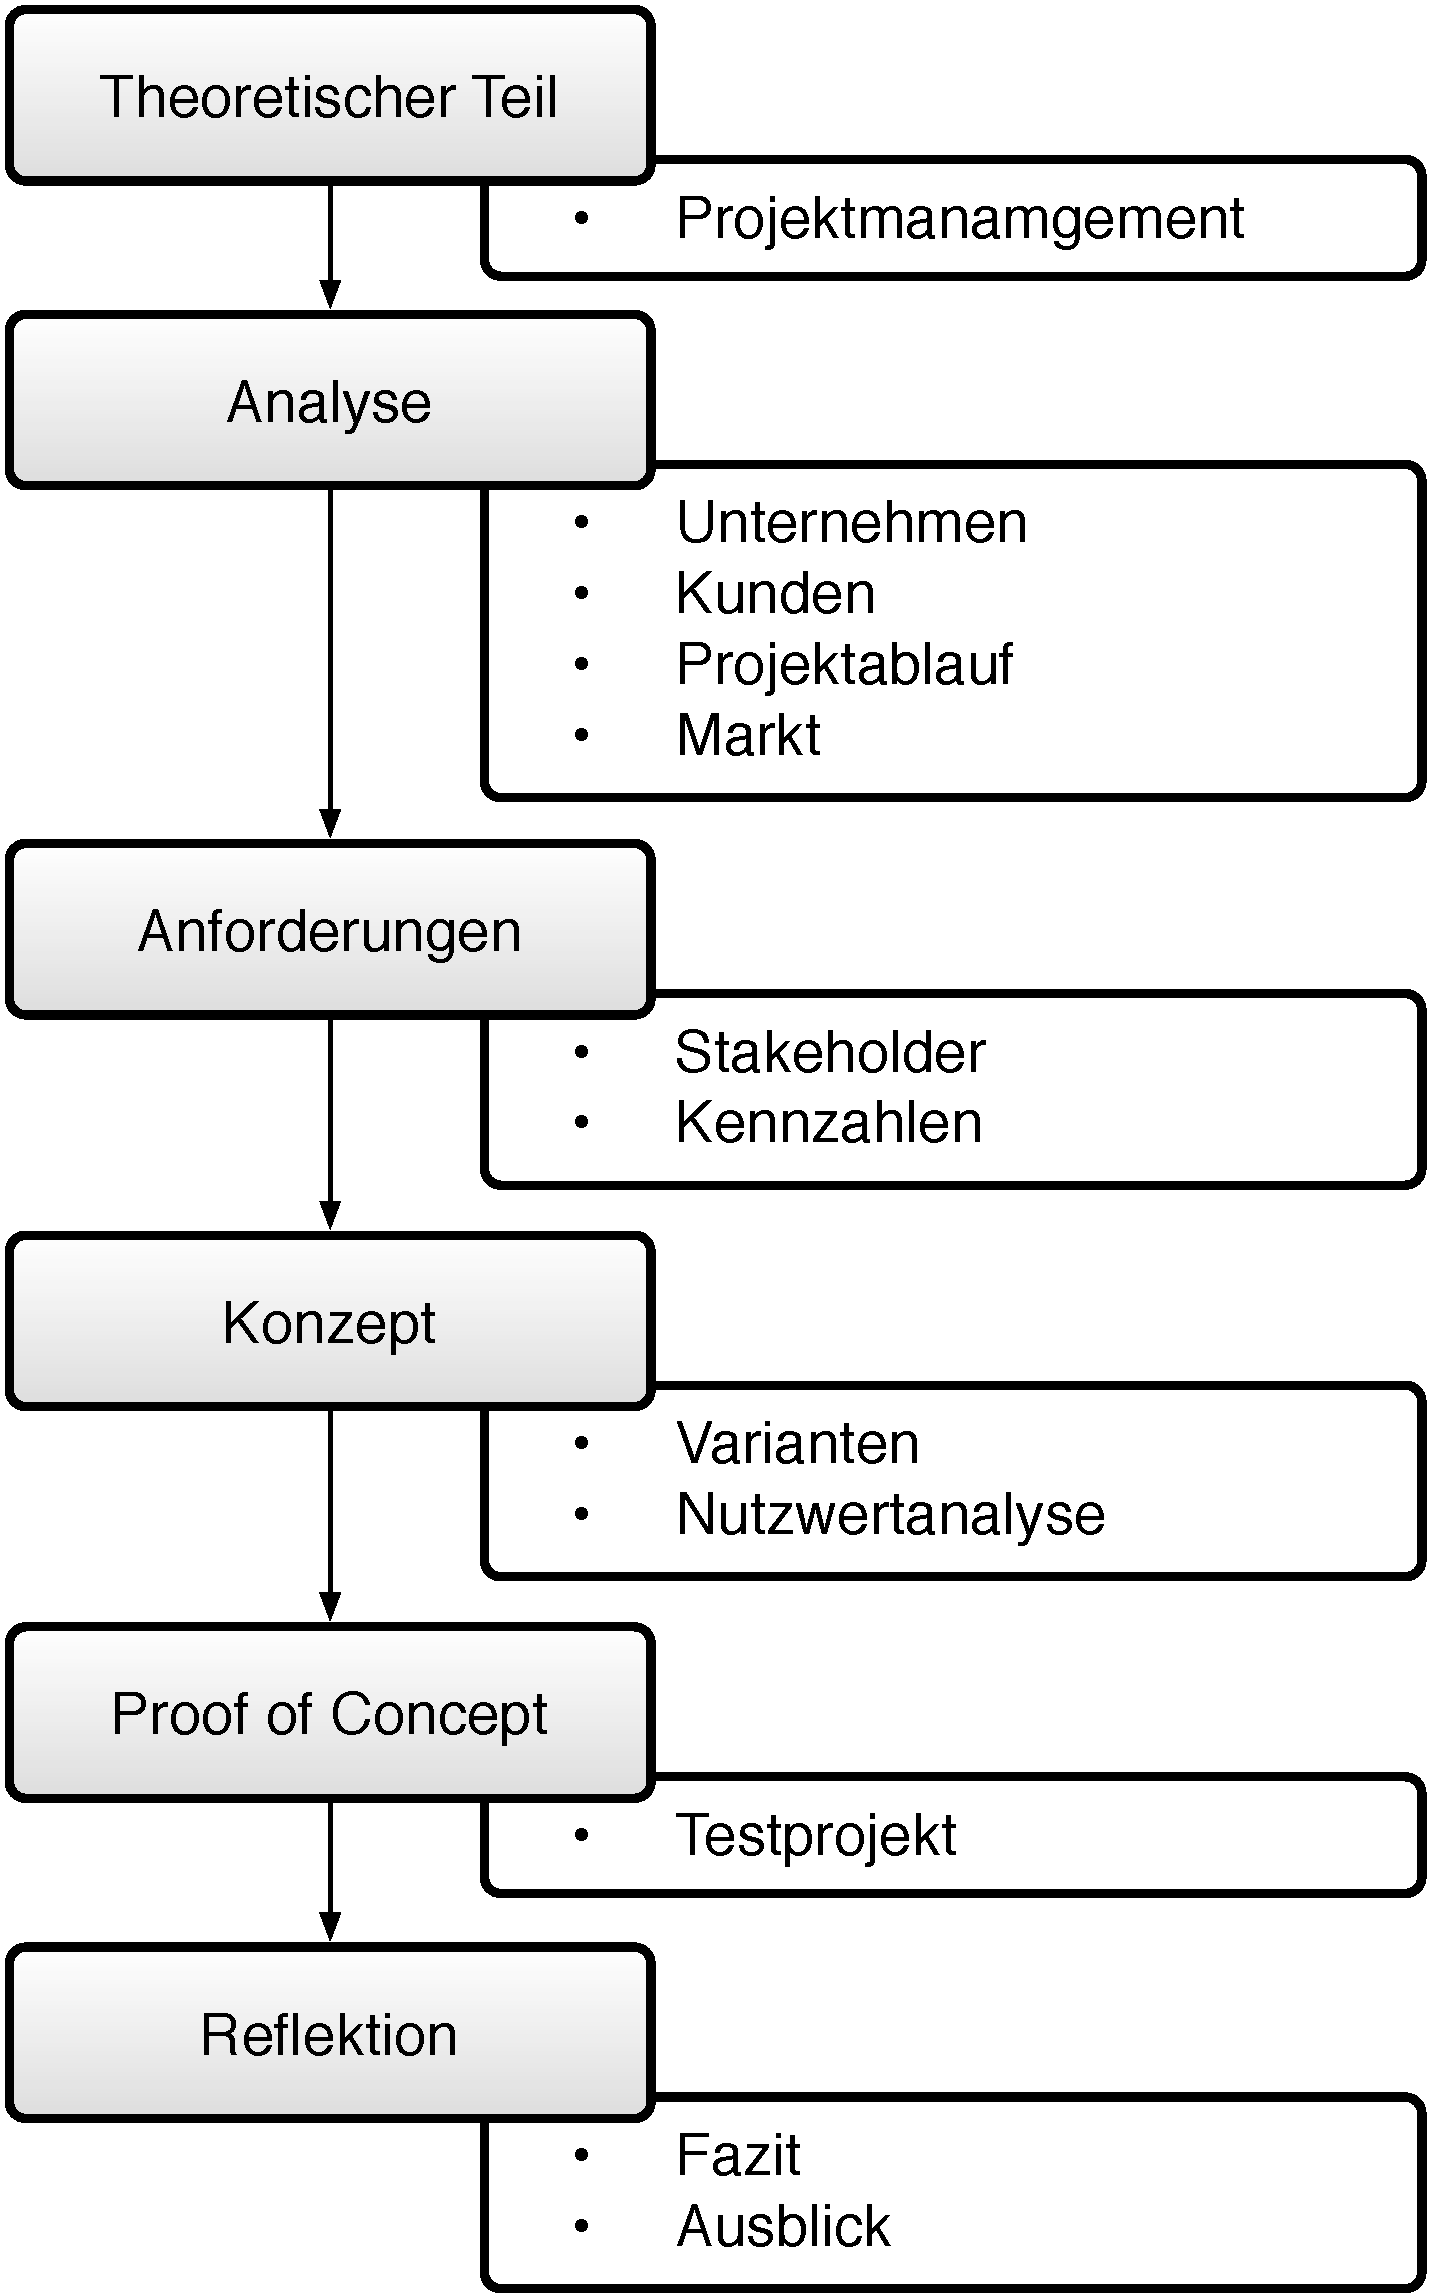
\includegraphics[width=0.6\textwidth,angle=0]{./bilder/einleitung/01_gliederung_arbeit.pdf}
\caption[Aufbau der Diplomarbeit]{Aufbau der Diplomarbeit\footnotemark}
\label{pic:01_gliederung_arbeit}
\end{center}
\end{figure}
\footnotetext{Eigene Darstellung}

\clearpage

\section{Inhaltliche Schwerpunkte}
Die inhaltlichen Schwerpunkte dieser Arbeit liegen in den folgenden Bereichen:

\begin{itemize}
    \item Einarbeitung Theorie Projektmanagement
    \item Analyse des aktuellen Projektablaufes der allink GmbH
    \begin{itemize}
        \item Darstellung des Projektablaufes
        \item Aufzeigen der Stärken und Schwächen
        \item Zurzeit verwendete Software und Hilfsmittel
    \end{itemize}
    \item Aufnahme der Bedürfnisse und Anforderungen an den Projektablauf
    \item Konzept eines neuen Projektablaufes in Form eines Lösungsansatzes
    \begin{itemize}
        \item Erarbeitung von praxisnahen Varianten
        \item Aufzeigen von unterstützender Software und Hilfsmittel
    \end{itemize}
    \item ``Proof of Concept'' des Projektablaufes mit den gewählten Varianten
    \item Fazit und Reflektion der Arbeit
\end{itemize}

Die Arbeit soll dem Leser und anderen Agenturen in einer ähnlichen Situation
aufzeigen, was für Herausforderungen bei einem Wachstum entstehen und wie
sie mit Hilfe von Veränderungen und Anpassungen bewältigt werden können.

\section{Inhaltliche Ein- und Abgrenzung}
Die Arbeit fokussiert sich auf eine Agentur. Es wird vertieft auf deren Probleme
und Herausforderungen eingegangen. Deshalb sind die Schlüsse die darin gezogen
werden nicht grundsätzlich für jede Agentur anwendbar. Es wird jedoch versucht, das
ganze so global wie möglich zu betrachten. Da zum Schluss aber eine für die
Agentur in der Praxis anwendbare neue Lösung gesucht wird, passt diese wohl
kaum in jede Firmenkultur. 
Zusätzlich grenzt sich die Arbeit von folgenden Punkten klar ab:

\begin{itemize}
    \item Die Analysen beschränken sich auf Recherchen im Internet und Büchern.
    \item Umfragen, Erhebungen sowie Feldstudien werden nur begrenzt im Rahmen
        von Interviews durchgeführt.
    \item Die definierten zu messenden Kennzahlen können in den Bereich der Betriebswirtschaft
        und Buchhaltung fallen. Es wird aber nicht näher auf deren Theorien eingegangen.
\end{itemize}

  
  
  \chapter{Theoretische Grundlagen Projektmanagement}\label{chap:theorie_teil}
  \section{Projektmanagement - Begriff}
Für das gemeinsame Verständnis des Begriffes ``Projektmanagement'' wird zuerst
eine Definition des Wortes gemacht. Diese Arbeit lehnt sich an diese 
Begriffsdefinition an. Danach wird näher auf den Aufbau eines
Projektablaufes eingegangen.

Im Rahmen eines Projektmanagement werden die diversen Aufgaben ganzheitlich in
einem Projekt eingebettet und unter Berücksichtigung der Parameter Kosten, Termine
und Qualität geplant und durchgeführt.\footnote{\citealp*[Vgl.][S. 9]{burghardt2007einfuehrung}}
Die Stiftung für Forschung und Beratung am Betriebswissenschaftlichen Institut 
(BWI) der ETH Zürich definiert den Begriff Projektmanagement wie folgt:

\begin{quote}
``Projektmanagement wird als Überbegriff aller planenden, überwachenden,
koordinierenden und steuernden Massnahmen verstanden, die für die Um- oder
Neugestaltung von Systemen (resp. Problemlösungen) erforderlich sind.''\footnote{\citealp*[S. 1.1]{stiftung1998projekt}}
\end{quote}

\section{Projektablauf}
Der Projektablauf gehört zu den Methoden und Techniken der Organisation. Als
Projekt bezeichnet man ein Vorhaben, das einmalig ist und einen definierten
Start- und Endtermin hat. Im Projektablauf regelt man die Ablauforganisation
eines Projektes, also welche Aufgaben wann zu erledigen sind.\footnote{\citealp*[Vgl.][S. 136]{schmidt2002einfuehrung}}
Das Projektmanagement mit dem Projektablauf als Methode umfasst alle Aktivitäten,
die für eine vollständige Abwicklung eines Projektes erforderlich sind.\footnote{\citealp*[Vgl.][S. 11]{burghardt2007einfuehrung}}

Ein Projektablauf unterteilt man in vier Hauptabschnitte, die in der Abbildung \ref{pic:01_hauptabschnitte}
dargestellten sind.

\clearpage

\begin{figure}[htbp]
\begin{center}

\includegraphics[width=0.85\textwidth,angle=0]{./bilder/theorie/01_hauptabschnitte.pdf}
\caption[Vier Hauptabschnitte eines Projektablaufes]{Vier Hauptabschnitte eines Projektablaufes\footnotemark}
\label{pic:01_hauptabschnitte}
\end{center}
\end{figure}
\footnotetext{Eigene Darstellung in Anlehnung an \citealp*[Bild 1.2]{burghardt2007einfuehrung}}

\subsection{Projektdefinition}
Die Projektdefinition besteht aus der eigentlichen Gründung eines Projektes,
der Definition des Projektziels und die Organisation des Projektes.

Zu Beginn eines Projektes steht der Projektantrag. Er beinhaltetet alle relevanten
Informationen wie eine Aufgabenbeschreibung und Termine. Wird der Projektantrag
angenommen, wandelt sich der Antrag in einen Projektauftrag um.\footnote{\citealp*[Vgl.][S. 13]{burghardt2007einfuehrung}}
Als nächstes muss ein eindeutiges und vollständiges Projektziel definiert werden.
Dies geschieht meist zusammen mit dem Auftraggeber anhand eines Anforderungskatalogs
oder Pflichtenhefts.

Es empfiehlt sich eine Problemfeldanalyse und eine Wirtschaftlichkeitsbetrachtung
zu machen. Ohne genauere Kenntnisse zur Wirtschaftlichkeit eines Projektes sollte
keines begonnen werden.\footnote{\citealp*[Vgl.][S. 45]{burghardt2007einfuehrung}}
Unter einer Problemfeldanalyse versteht man eine klare Definition des eigentlichen
Problems, wobei das Problem eher als Herausforderung zu betrachten ist. Man
stellt sich dabei folgende Fragen:

\begin{itemize}
    \item Was ist das Problem bzw. die Herausforderung?
    \item Wer sind die Betroffenen und die Beteiligten?
    \item Was sind deren wichtigste Ziele?
\end{itemize}

Bei der Überprüfung der Wirtschaftlichkeit eines Projektes kann dies im Sinne
des Endproduktes oder des Auftrages geschehen. Im Ersteren versucht man zu
errechnen, ob das Endprodukt einen wirtschaftlichen Nutzen für den Auftraggeber
darstellt. Dies sollte der Auftraggeber normalerweise schon selbst vorgenommen
haben. Für die Projektleitung steht schlussendlich der wirtschaftliche Nutzen
des Auftrages für die eigene Unternehmung im Vordergrund.

Ist dies zutreffend, müssen die organisatorischen Voraussetzungen für das Projekt geschaffen werden,
indem der Projektleiter ernannt und eine passende Projektorganisation gewählt wird.
Die Definition einer Projektorganisation lautet nach DIN 69901:

\begin{quote}
``Gesamtheit der Organisationseinheiten und der aufbau- und ablauforganisatorischen
Regelungen zur Abwicklung eines bestimmten Projektes.''\footnote{Vgl. DIN 69901}
\end{quote}

Je nach Bereichsüberschreitung innerhalb des Unternehmens und der einzubindenden
Projektmitarbeiter sowie der Bedeutung und der Grösse des Projektes kann zwischen
fünf Formen von Projektorganisationen unterschieden werden:\footnote{\citealp*[Vgl.][S. 56]{burghardt2007einfuehrung}}

\begin{itemize}
    \item Reine Projektorganisation
    \item Einfluss-Projektorganisation
    \item Matrix-Projektorganisation
    \item Auftrags-Projektorganisation
    \item Projektmanagement in der Linie
\end{itemize}

In der reinen Projektorganisation wird in der bestehenden Unternehmensstruktur
eine zusätzliche Stelle für das Projekt geschaffen und alle beteiligten 
Projektmitarbeiter unter einem Projektleiter, der die Linienautorität hat, 
zusammengefasst.\footnote{\citealp*[Vgl.][S. 56]{burghardt2007einfuehrung}}
In der Grafik \ref{pic:05_projektorganisationen_reine} ist 
ein Beispiel einer reinen Projektorganisation abgebildet.

\begin{figure}[htbp]
\begin{center}
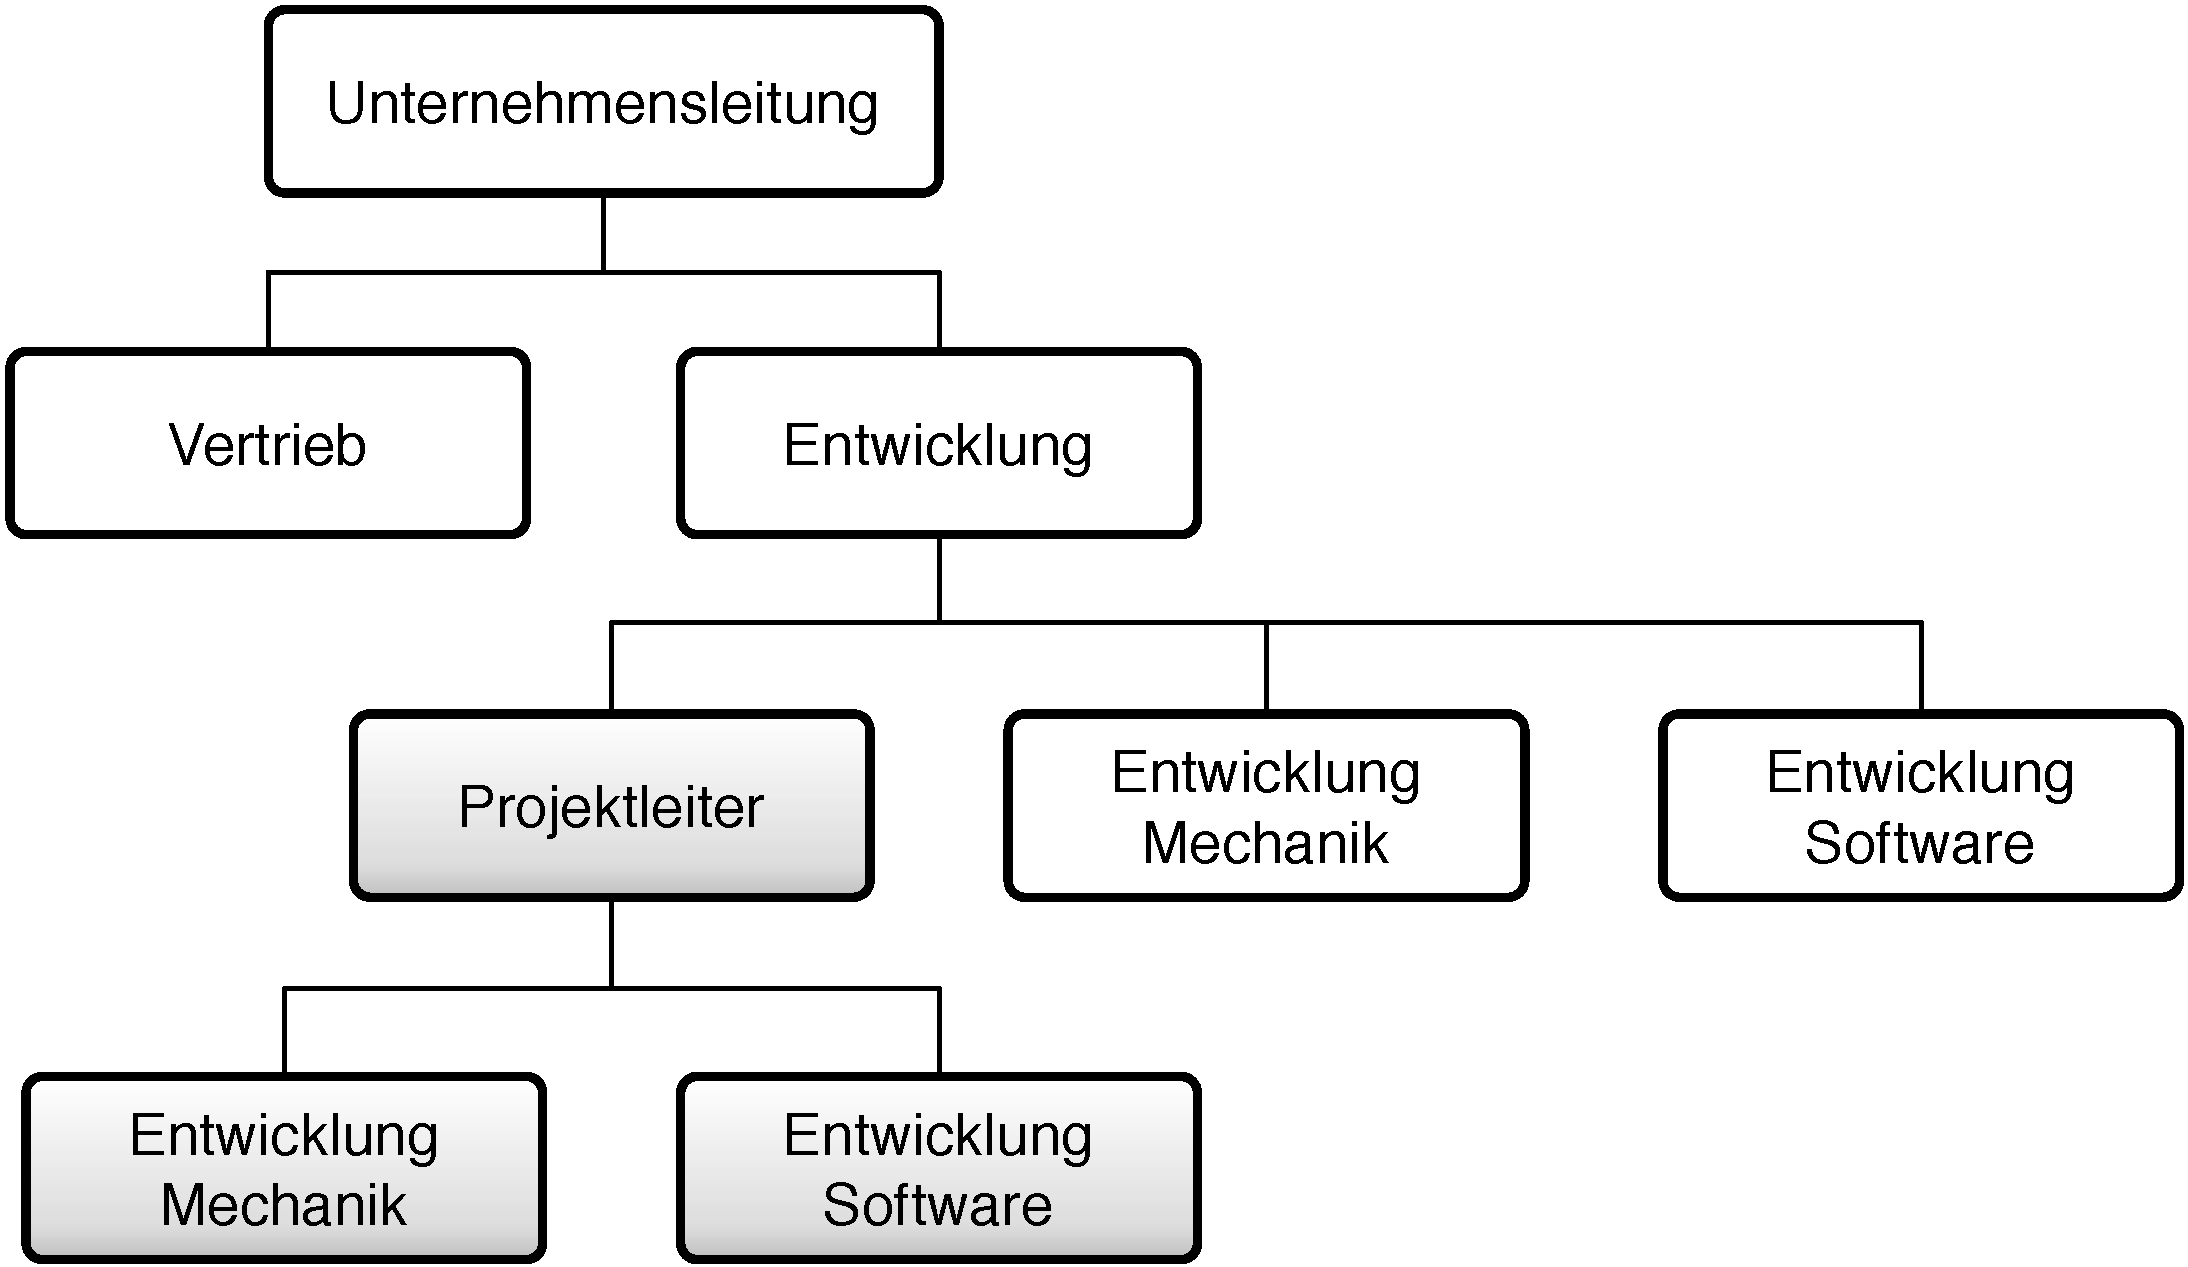
\includegraphics[width=0.5\textwidth,angle=0]{./bilder/theorie/05_projektorganisationen_reine.pdf}
\caption[Reine Projektorganisation]{Reine Projektorganisation\footnotemark}
\label{pic:05_projektorganisationen_reine}
\end{center}
\end{figure}
\footnotetext{Eigene Darstellung in Anlehnung an \citealp*[Bild 2.9]{burghardt2007einfuehrung}}

In einer Einlfuss-Projektorganisation gibt es anstelle eines Projektleiters
einen Projektkoordinator, der als Stabsstelle eingefügt wird. Er hat jedoch kaum
Kompetenzen und kann nur koordinierend und lenkend wirken.\footnote{\citealp*[Vgl.][S. 57]{burghardt2007einfuehrung}}
In der Grafik \ref{pic:05_projektorganisationen_einfluss}
ist ein Beispiel einer Einfluss-Projektorganisation abgebildet.

\begin{figure}[htbp]
\begin{center}
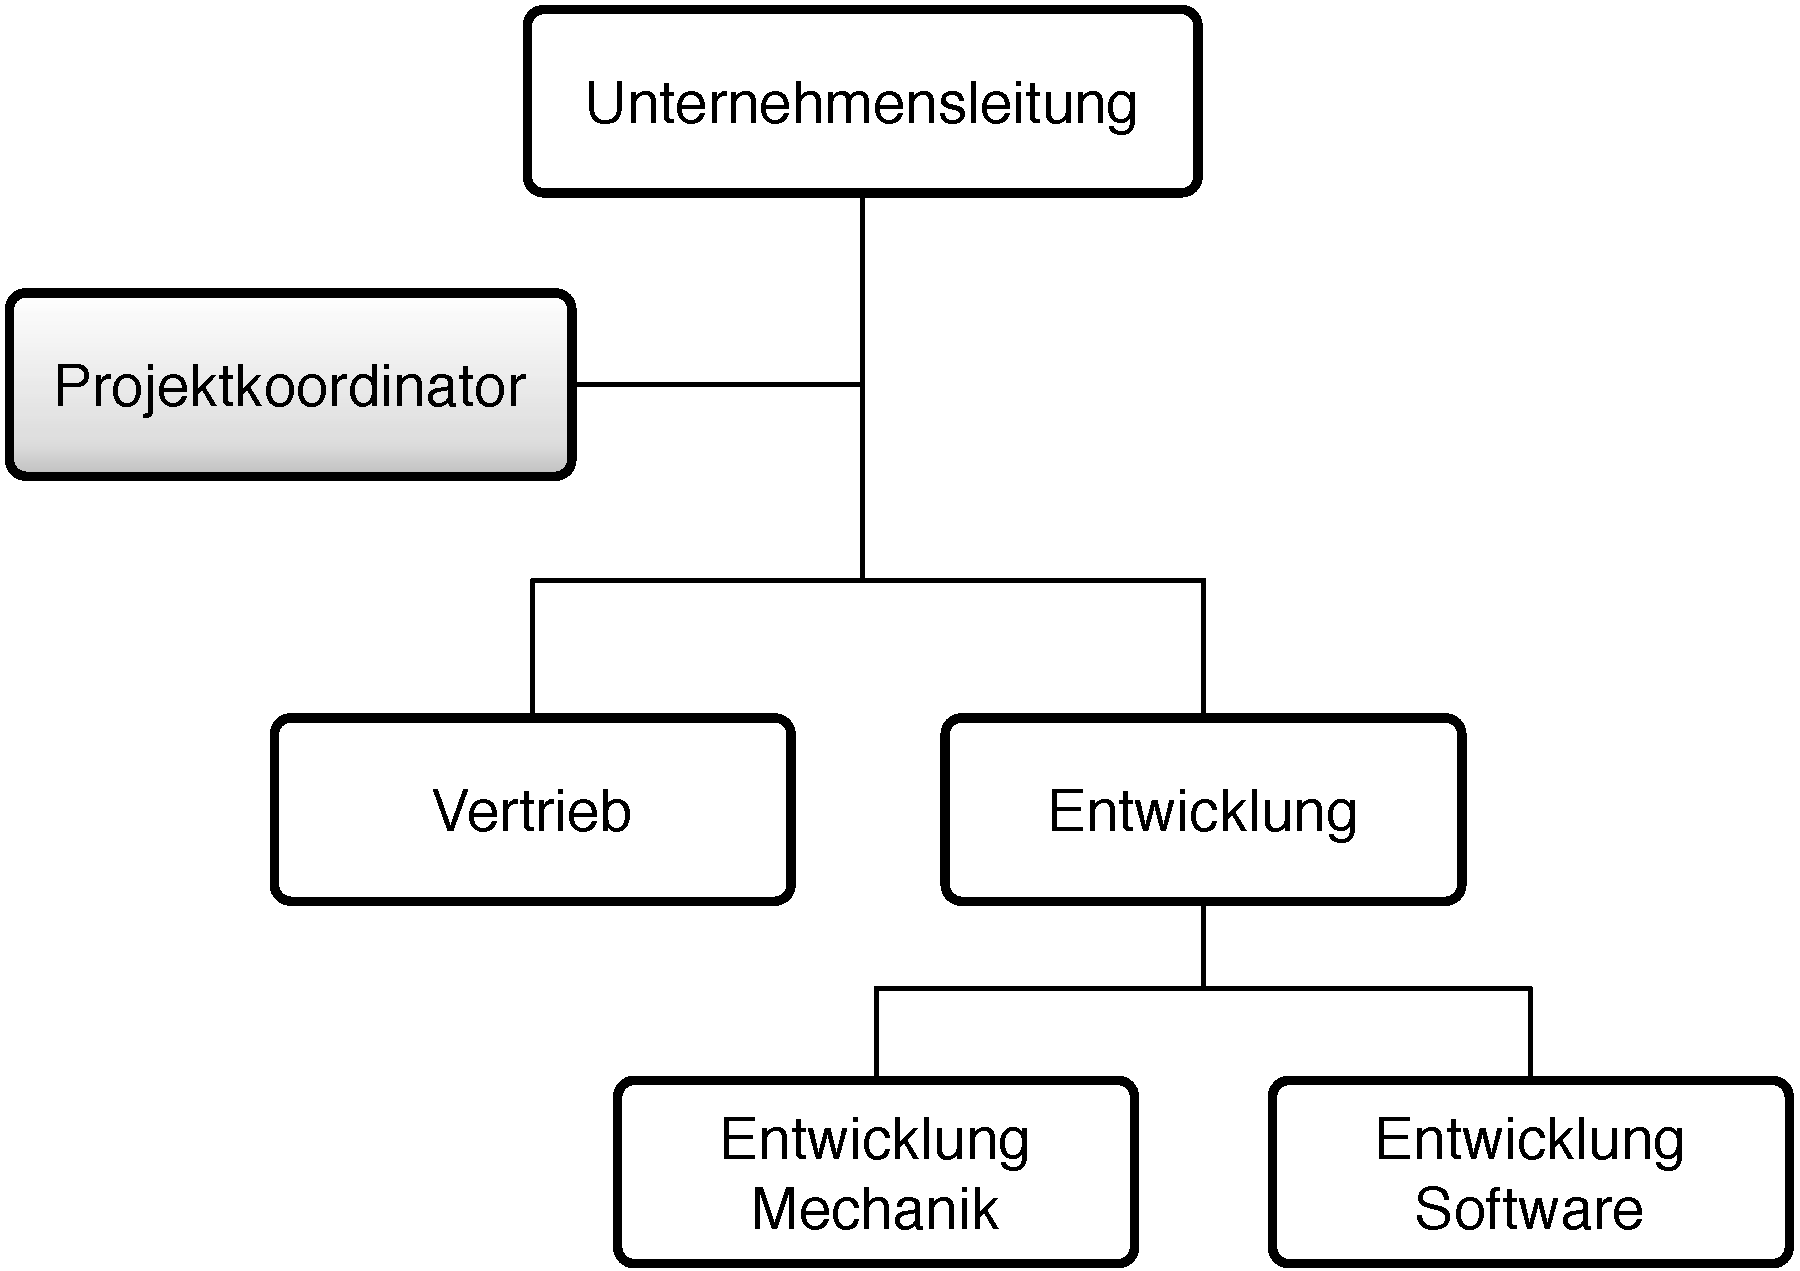
\includegraphics[width=0.45\textwidth,angle=0]{./bilder/theorie/05_projektorganisationen_einfluss.pdf}
\caption[Einfluss-Projektorganisation]{Einfluss-Projektorganisation\footnotemark}
\label{pic:05_projektorganisationen_einfluss}
\end{center}
\end{figure}
\footnotetext{Eigene Darstellung in Anlehnung an \citealp*[Bild 2.10]{burghardt2007einfuehrung}}

In der Matrix-Projektorganisation trägt der Projektleiter zwar die ganze Verantwortung
des Projektes, hat aber nicht die ganze Weisungsbefugnis für alle beteiligten Mitarbeiter.
Die fachliche Weisungsbefugnis unterliegt zwar dem Projektleiter, die disziplinarische
bleibt jedoch weiterhin beim direkten Vorgesetzten in der Linienorganisation.\footnote{\citealp*[Vgl.][S. 58]{burghardt2007einfuehrung}}
In der Grafik \ref{pic:05_projektorganisationen_matrix} ist ein Beispiel einer 
Matrix-Projektorganisation abgebildet.

\begin{figure}[htbp]
\begin{center}
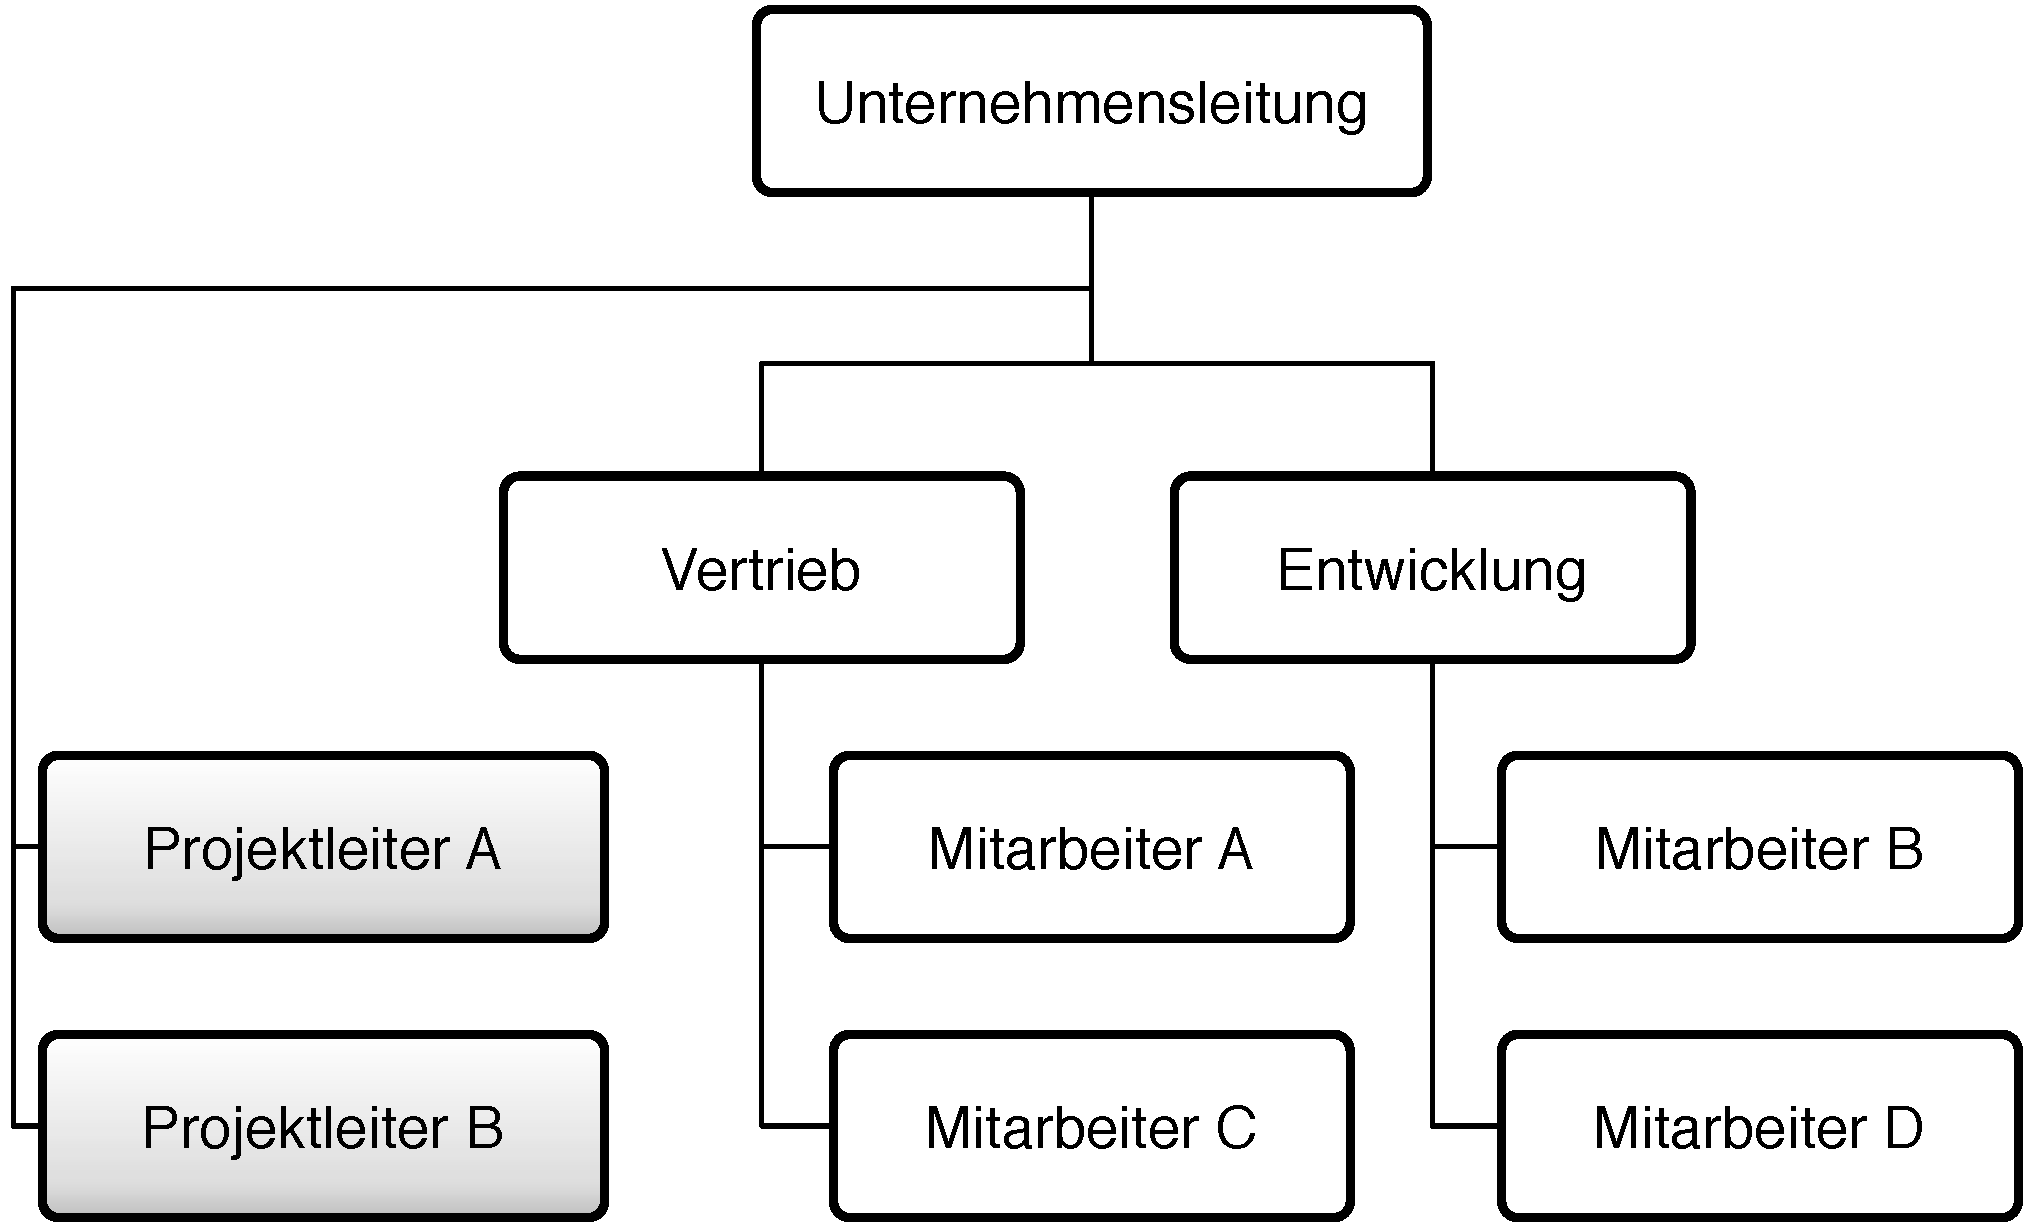
\includegraphics[width=0.5\textwidth,angle=0]{./bilder/theorie/05_projektorganisationen_matrix.pdf}
\caption[Matrix-Projektorganisation]{Matrix-Projektorganisation\footnotemark}
\label{pic:05_projektorganisationen_matrix}
\end{center}
\end{figure}
\footnotetext{Eigene Darstellung in Anlehnung an \citealp*[Bild 2.11]{burghardt2007einfuehrung}}

Die Auftrags-Projektorganisation ist ebenfalls eine matrixorientierte 
Organisationsform. Bei dieser gibt es aber keine Doppelunterstellung der Mitarbeiter.
Somit ist hier der Projektleiter auch für die fachtechnische Durchführung des
Projektes verantwortlich.\footnote{\citealp*[Vgl.][S. 58]{burghardt2007einfuehrung}}
In der Grafik \ref{pic:05_projektorganisationen_auftrags}
ist ein Beispiel einer Auftrags-Projektorganisation abgebildet.

\clearpage

\begin{figure}[htbp]
\begin{center}
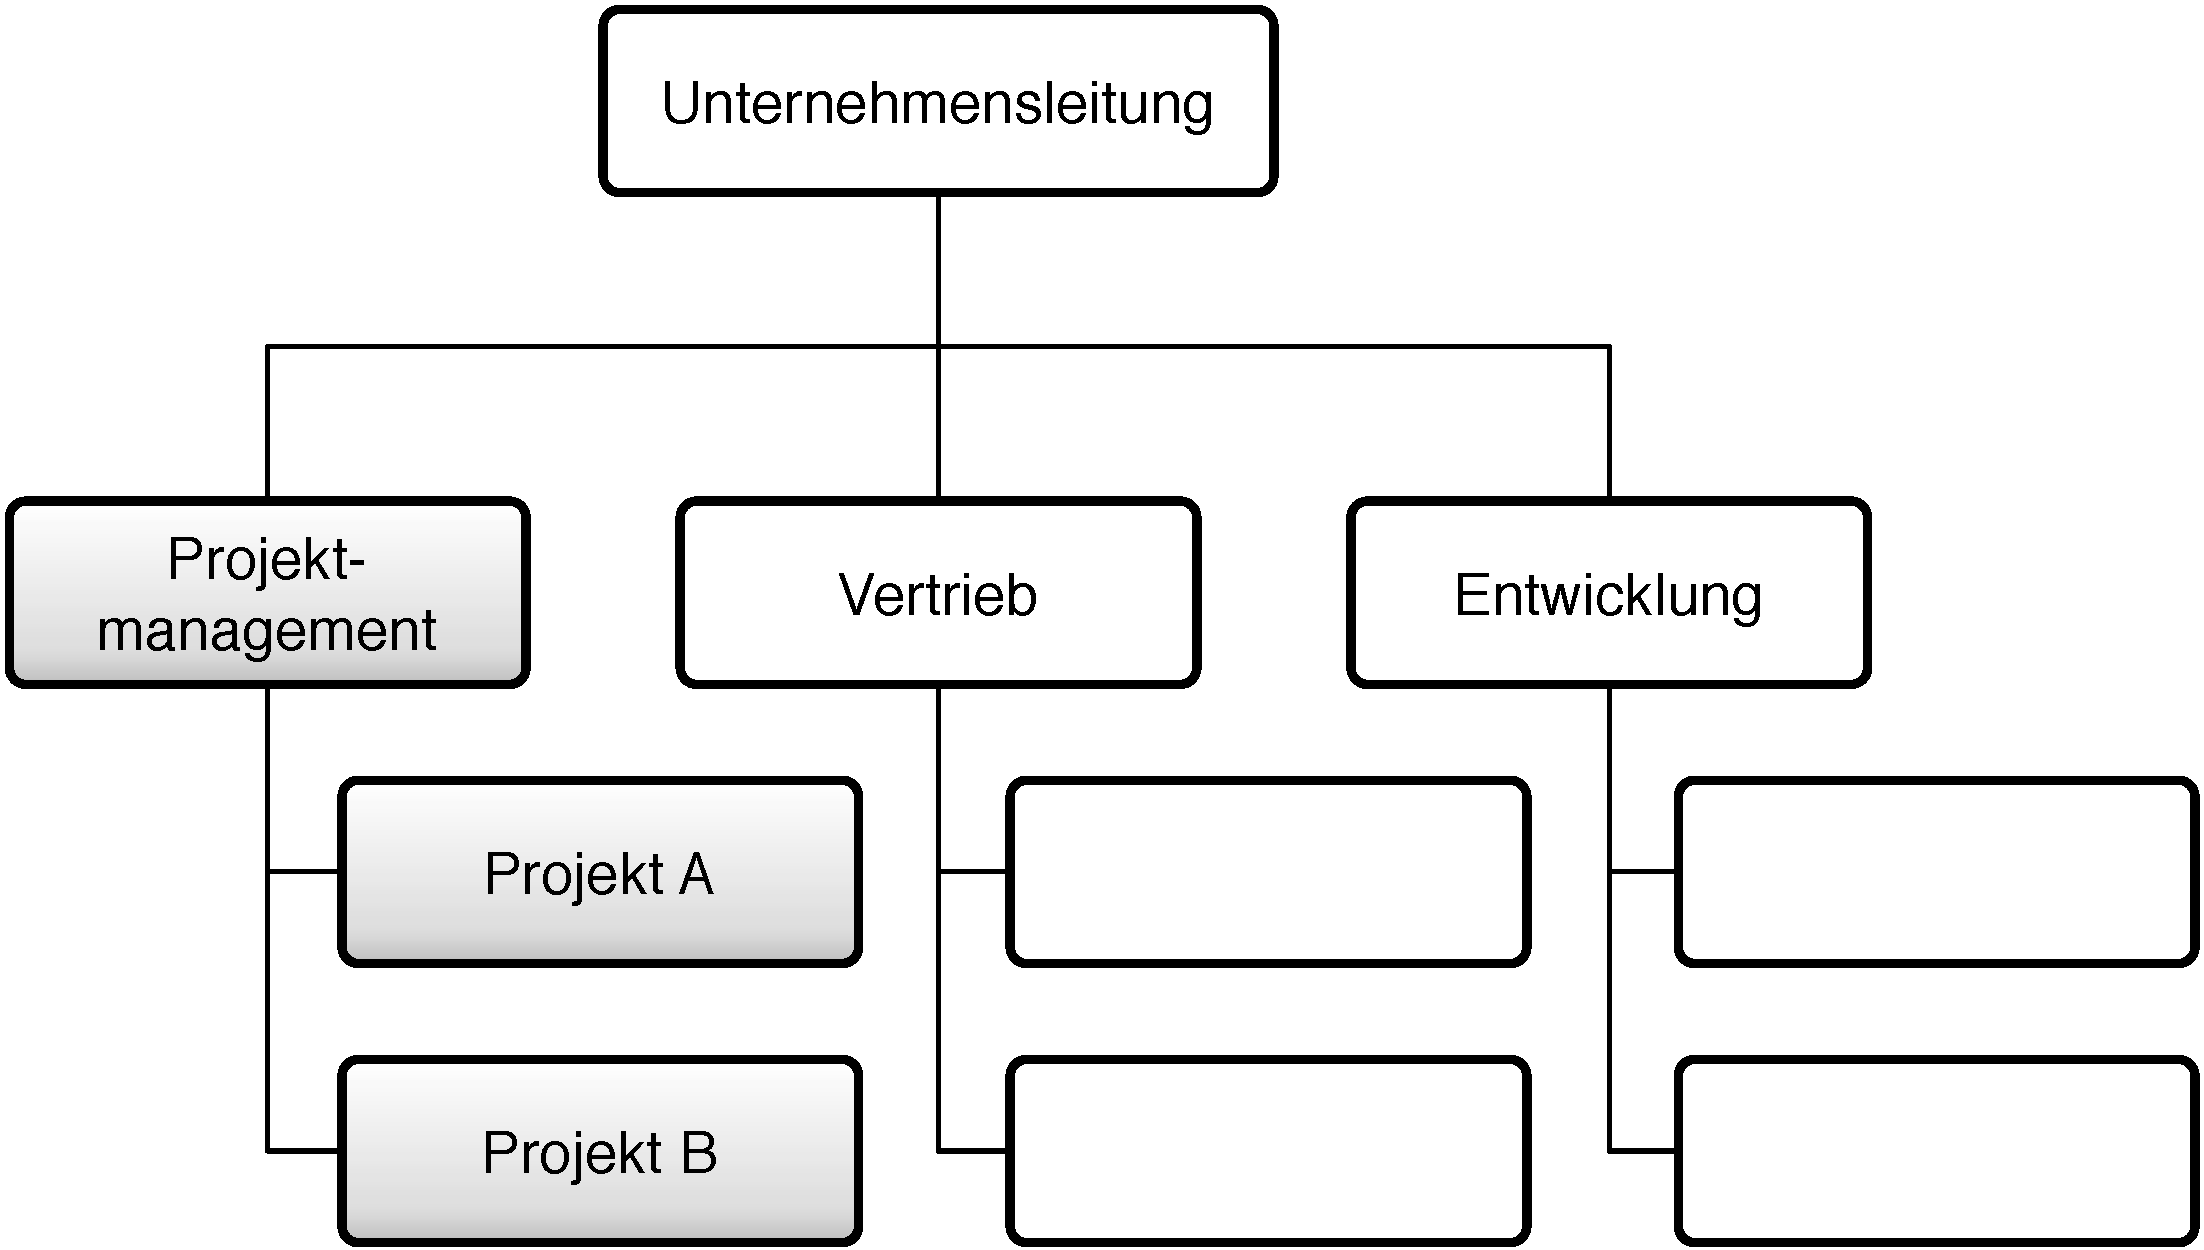
\includegraphics[width=0.55\textwidth,angle=0]{./bilder/theorie/05_projektorganisationen_auftrags.pdf}
\caption[Auftrags-Projektorganisation]{Auftrags-Projektorganisation\footnotemark}
\label{pic:05_projektorganisationen_auftrags}
\end{center}
\end{figure}
\footnotetext{Eigene Darstellung in Anlehnung an \citealp*[Bild 2.12]{burghardt2007einfuehrung}}

Die Durchführung eines Projektes erfordert nicht immer das Einrichten einer eigenen
Projektorganisation. Beim Projektmanagement über die Linie wird ebenfalls ein
Projektleiter ernannt, der dann meist eine Art Gruppenführer-Funktion einnimmt,
ähnlich wie bei der Einfluss-Projektorganisation.

\subsection{Projektplanung}
In der Projektplanung definiert man die Strukturplanung, eine Aufwandschätzung,
die Arbeits- und Kostenplanung sowie das Risikomanagement.

In der Strukturplanung wird das Vorhaben technisch, aufgabengemäss und kaufmännisch
anhand den Anforderungen strukturiert. Auf den sich ergebenden Strukturen bauen
alle weiteren Planungsschritte auf. Danach werden daraus die einzelnen Aufgabenpakete
abgeleitet, für die dann eine Aufwandsschätzung durchzuführen ist.\footnote{\citealp*[Vgl.][S. 14]{burghardt2007einfuehrung}}
Wenn möglich sollten zur Schätzung nebst dem eigenen Erfahrungspotential auch
Erfahrungen von Experten zum Thema herangezogen werden.

Ein allgemeines Schema zur Vorgehensweise zum Sammeln von Erfahrungswerten zur 
Aufwandsschätzung ist in der Grafik \ref{pic:02_schema_aufwandsschaetzung}
abgebildet.

\clearpage

\begin{figure}[htbp]
\begin{center}
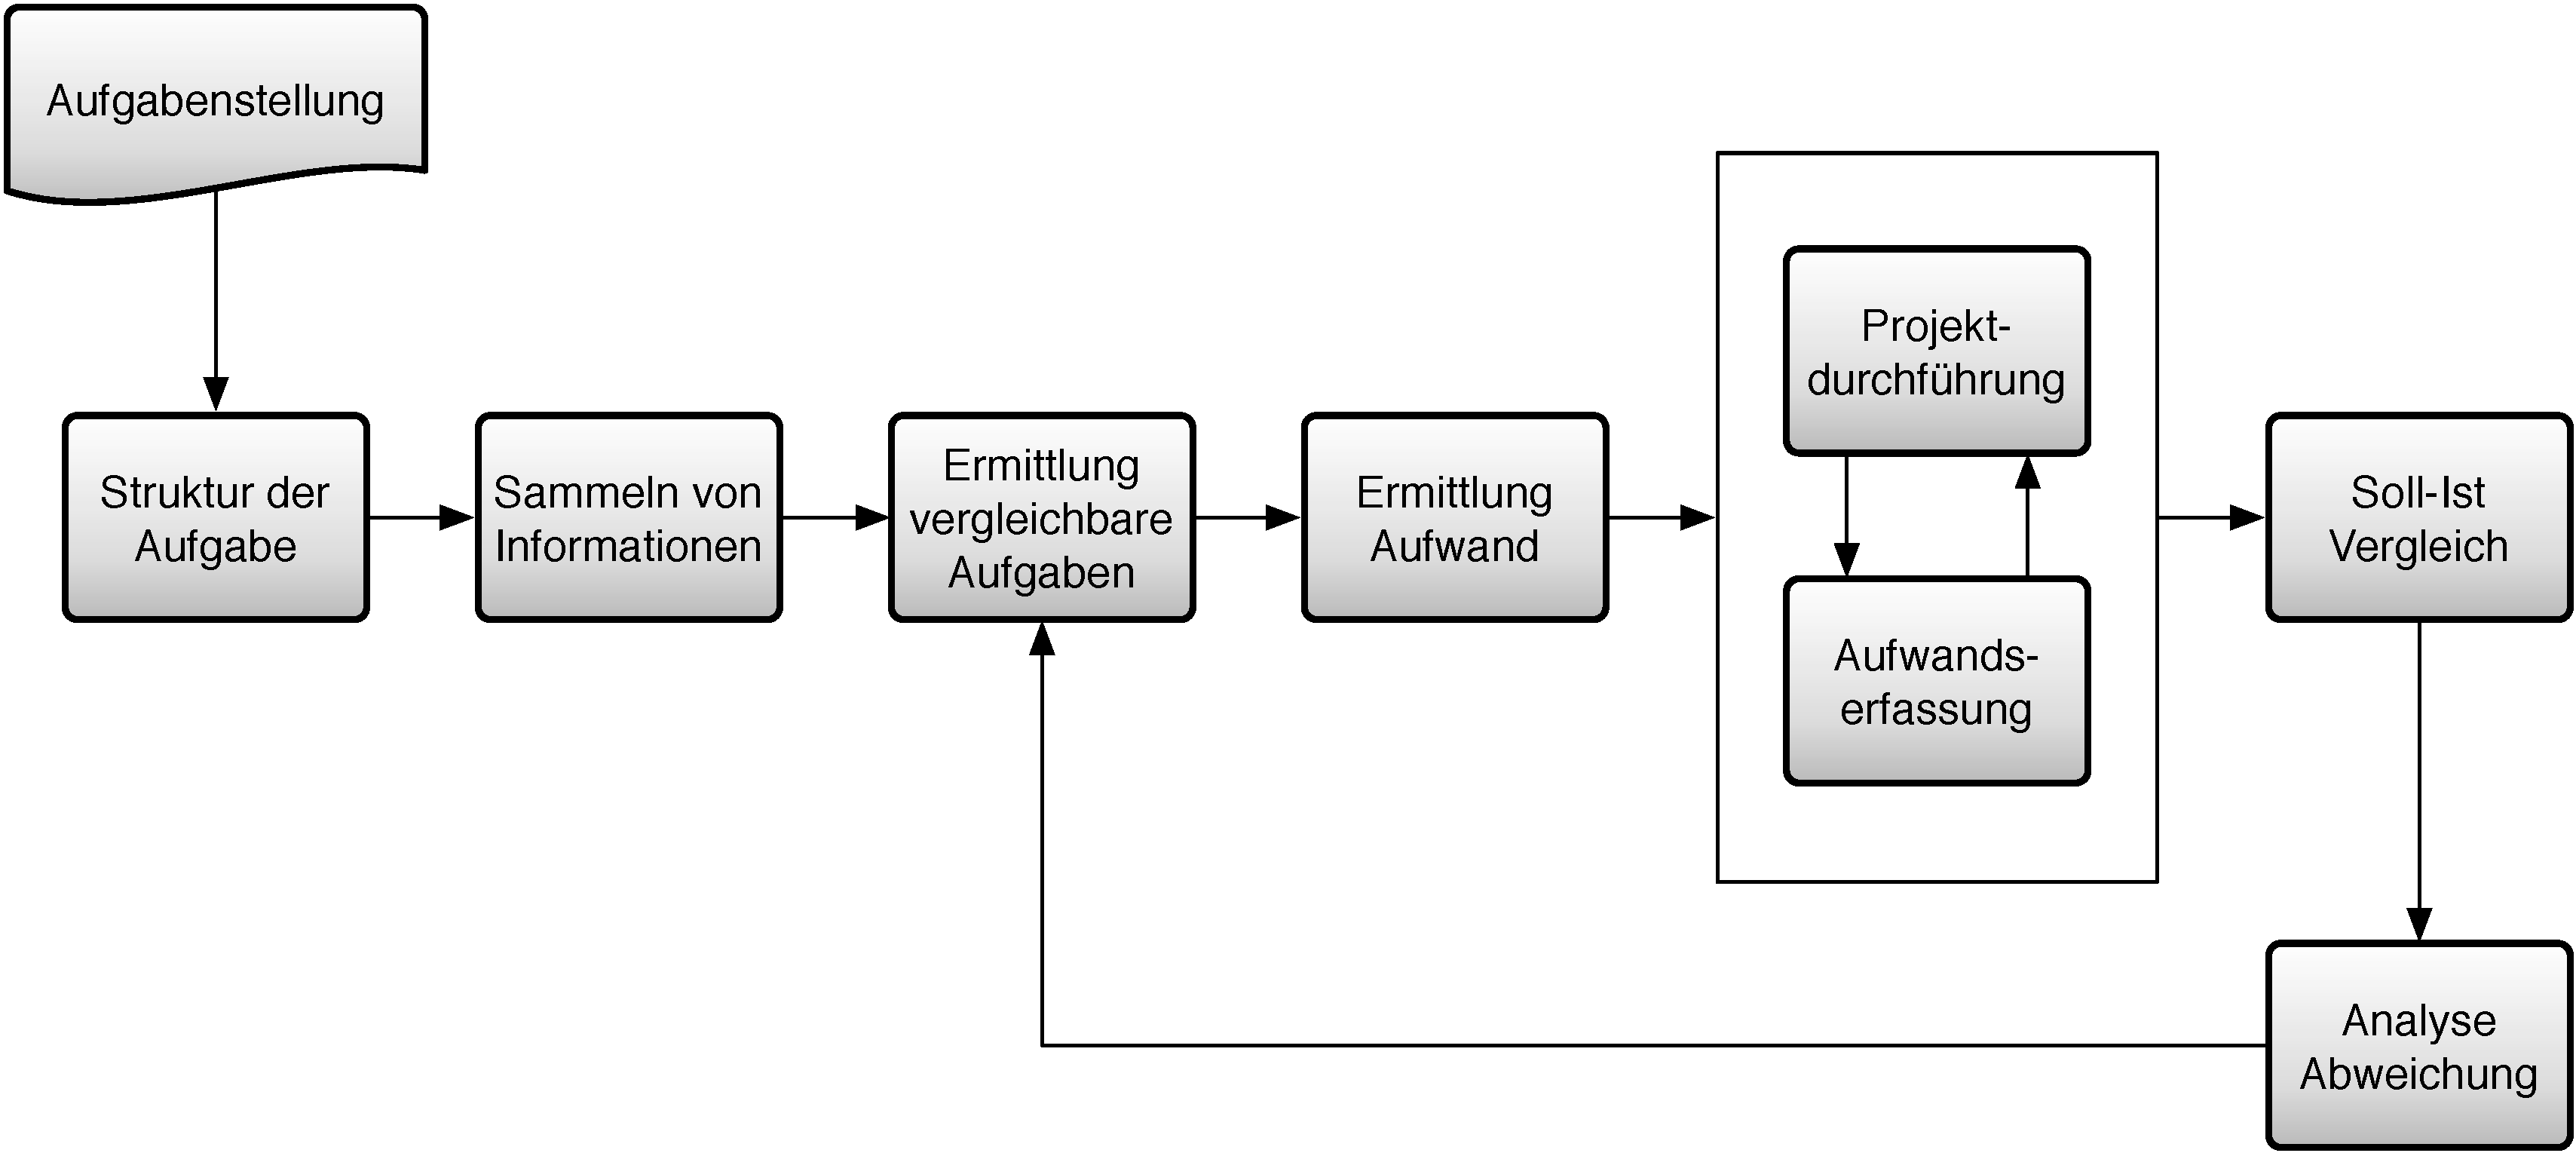
\includegraphics[width=0.75\textwidth,angle=0]{./bilder/theorie/02_schema_aufwandsschaetzung.pdf}
\caption[Sammeln von Erfahrungswerten zur Aufwandsschätzung]{Sammeln von Erfahrungswerten zur Aufwandsschätzung\footnotemark}
\label{pic:02_schema_aufwandsschaetzung}
\end{center}
\end{figure}
\footnotetext{Eigene Darstellung des Schemas in Anlehnung an \citealp*[S. 112]{litke2007projektmanagement}}

Es gibt diverse Aufwandsschätzungsverfahren die genutzt werden können. Die Methoden unterscheiden
sich beim Schätzverfahren und können zum Beispiel nach folgender Klassifikation 
erfolgen:\footnote{Vgl. \citealp*{noth1986aufwandschaetzung} und \citealp*{knoell1991aufwandsschaetzung}}

\begin{itemize}
    \item Anzahl der Phasen, die abgedeckt werden, zum Beispiel:
    \begin{itemize}
        \item Einzelaktivitäten
        \item Programmierung
        \item Detailentwurf und Programmierung
        \item Gesamter Entwicklungsprozess
    \end{itemize}
    \item Theoretische oder praktische Absicherung, zum Beispiel:
    \begin{itemize}
        \item Unternehmensspezifische Verfahren
        \item Unternehmensunabhängige Praxisverfahren
        \item Wissenschaftlich fundierte Verfahren
    \end{itemize}
    \item Verwendungszweck, zum Beispiel:
    \begin{itemize}
        \item Kosten/Nutzenanalyse zur Kalkulation der Kosten
        \item Kapazitäts- und Terminplanung zur Ermittlung von Plangrössen
    \end{itemize}
\end{itemize}

Anhand der Ergebnisse aus der Aufwandsschätzung werden nun die einzelnen
Arbeitspakete bzw. Teilaufgaben in eine Arbeitsplanung übernommen. Oft empfiehlt
es sich hier einen Netzplan zur Erstellung der Aufgaben- und Terminplanung
anzufertigen. 

``Die Netzplantechnik ist trotz aller Kritik eines der leistungsfähigsten 
Projektmanagement-Hilfsmittel, wenn sie richtig eingesetzt wird.''\footnote{\citealp*[S. 14]{burghardt2007einfuehrung}}

\begin{figure}[htbp]
\begin{center}
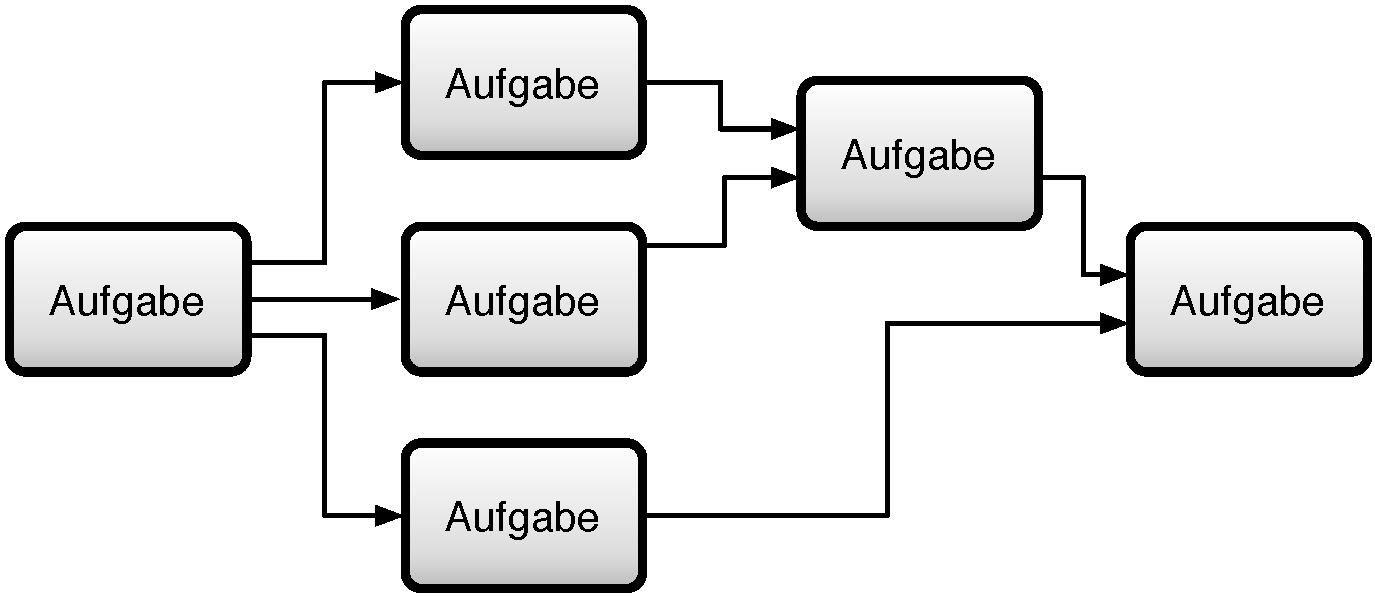
\includegraphics[width=0.5\textwidth,angle=0]{./bilder/theorie/03_darstellung_netzplan.pdf}
\caption[Konzeptionelle Darstellung eines determinisitischen Netzplanes]{Konzeptionelle 
    Darstellung eines determinisitischen Netzplanes\footnotemark}
\label{pic:03_darstellung_netzplan}
\end{center}
\end{figure}
\footnotetext{Eigene Darstellung des Schemas in Anlehnung an \citealp*[Bild 3.17]{burghardt2007einfuehrung}}

% http://books.google.de/books?id=m54LKbnCIoYC&pg=PA155&dq=Netzplantechnik&hl=de&ei=Qai-Tf2dNsmDOqL12dsF&sa=X&oi=book_result&ct=result&resnum=9&ved=0CHYQ6AEwCA#v=onepage&q=Netzplantechnik&f=false

\subsection{Projektkontrolle}
An erster Stelle der Projektkontrolle steht der Plan/Ist-Vergleich der vorgegebenen
Projektparameter. Durch einen laufenden Vergleich im Rahmen der Projektkontrolle
erreicht man, dass Abweichungen frühzeitig erkannt werden. Diese Abweichungen
führen zu ``geeigneten'' Massnahmen, die rechtzeitig ergriffen werden können.
Die Projektkontrolle umfasst im ganzen die Termin-, Aufwands-, Kosten-, 
und Sachfortschrittskontrolle, Qualitätssicherung, Projektdokumentation und
das Personalmanagement.\footnote{\citealp*[Vgl.][S. 15]{burghardt2007einfuehrung}}

Die Terminkontrolle wird in der Praxis so umgesetzt, dass die Einhaltung
und Erreichung der gesetzten Meilensteine kontrolliert wird. Wenn ein 
Meilenstein nicht eingehalten werden kann, muss kontrolliert werden, ob die
weiteren davon betroffen sind. Häufig ist das der Fall und die Termine
müssen angepasst und neu gewählt werden. Hierbei ist es wichtig, den Auftraggeber
über die Veränderungen zu informieren.

Die Aufwands- und Kostenkontrolle wird in der Praxis meist durch die Kontrolle
der rapportierten Stunden durchgeführt. Man sollte in beiden Fällen, also der
Termin- und Aufwandskontrolle, eine Trendanalyse erstellen, um eine mögliche
Entwicklung daraus abzuleiten.

\clearpage

In der Praxis werden immer wieder folgende, in der Grafik \ref{pic:06_trendanalyse}
abgebildeten, sechs typische Kurvenverläufe beobachtet.\footnote{\citealp*[Vgl.][S. 177 und S. 194]{burghardt2007einfuehrung}}

\begin{figure}[htbp]
\begin{center}
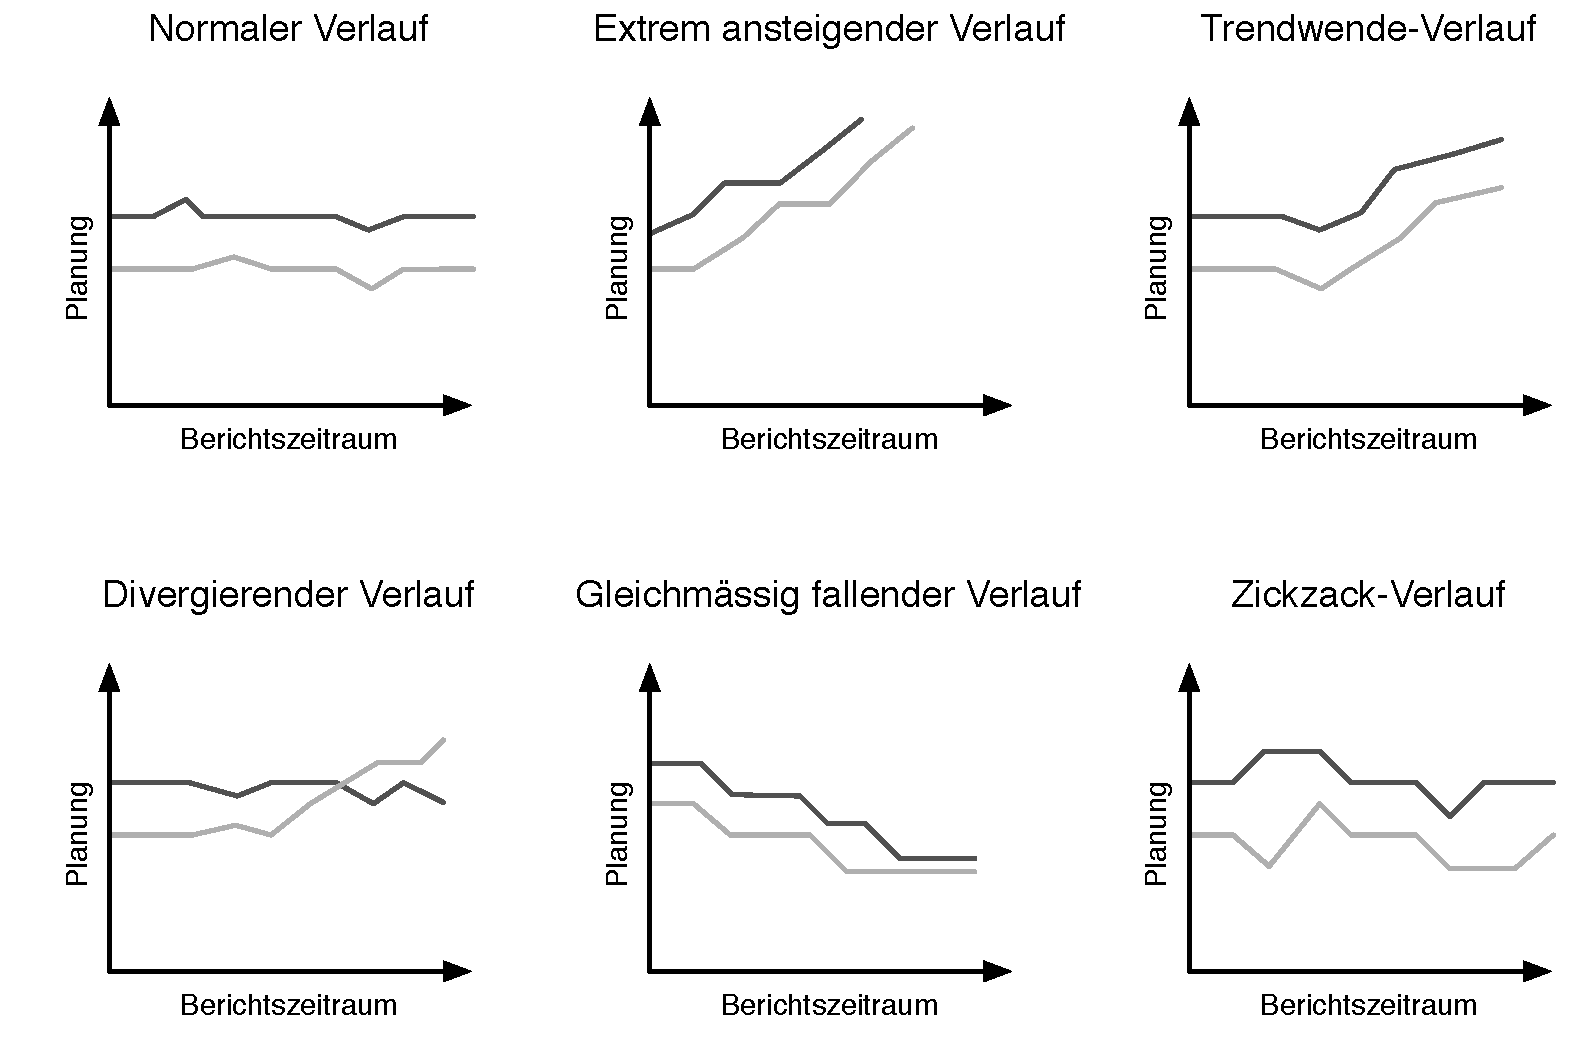
\includegraphics[width=0.8\textwidth,angle=0]{./bilder/theorie/06_trendanalyse.pdf}
\caption[Typische Kurvenverläufe bei Trendanalysen]{Typische Kurvenverläufe bei Trendanalysen\footnotemark}
\label{pic:06_trendanalyse}
\end{center}
\end{figure}
\footnotetext{Eigene Darstellung des Schemas in Anlehnung an \citealp*[Bild 4.4 und 4.13]{burghardt2007einfuehrung}}

\begin{description}
    \item [Normaler Verlauf] Hier sind geringe Termin- und Kostenverschiebungen 
    ablesbar. Mit hoher Wahrscheinlichkeit kann der Gesamttermin und das Budget 
    eingehalten werden.

    \item [Extrem ansteigender Verlauf] Hier wurde anscheinend laufend zu optimistisch geplant 
    und budgetiert. Der Endtermin wird sich mit hoher Wahrscheinlichkeit erheblich 
    verschieben und das Budget wird nicht eingehalten werden können.

    \item [Trendewende-Verlauf] Hier wurden möglicherweise die geplanten Termine 
    und Budgets künstlich eingehalten und die ``Probleme'' nach hinten verschoben. 
    Gegen Ende zeichnet sich eine erhebliche Veränderung ab. Ein rechtzeitiger 
    korrigierender Eingriff wurde dadurch verhindert.

    \item [Divergierender Verlauf] Gehen die Kurven auseinander, kann man ebenfalls 
    von einer falschen Rapportierung ausgehen. Man sollte die Trendanalyse im 
    Nachhinein ganz überarbeiten und korrigieren.
    
    \item [Gleichmässig fallender Verlauf] Hier wurde anscheinend mit einem sehr 
    grossen Sicherheitspuffer geplant. In so einem Fall ist es wichtig, seine
    Aufwandsschätzung am Ende des Projektes korrigiert in die Erfahrung einfliessen
    zu lassen, damit man in Zukunft genauer plant.
    
    \item [Zickzack-Verlauf] Ein solcher Verlauf deutet auf eine grosse
    Unsicherheit bezüglich des Fortschrittes hin. Mit grosser Wahrscheinlichkeit
    wird der Endtermin auch hier nicht eingehalten werden können.
\end{description}

Die Sachfortschrittskontrolle ist eine der wichtigsten Kontrollaufgaben für
den Projektleiter. Es ist zugleich aber auch die schwierigste, da oft keine
unmittelbaren Messgrössen vorhanden sind.
Die Kernfragen, die man sich in der Sachfortschrittskontrolle stellt, sind folgende:\footnote{\citealp*[Vgl.][S. 134]{jenny2009projektmanagement}}

\begin{itemize}
    \item Wie verhält sich der Projektaufwand zu den erbrachten Leistungen?
    \item Wie hoch ist der Zielerreichungsgrad der definierten Projektziele?
\end{itemize}

Es wird empfohlen, während der Projektdurchführung mehrmals eine Restaufwands-
und Restzeitschätzung vorzunehmen und die Trendanalysen zu aktualisieren.\footnote{\citealp*[Vgl.][S. 16]{burghardt2007einfuehrung}}

Bei der Projektdokumentation handelt es sich um die vollständigen Informationen
über das zu entwickelnde Produkt. Es empfiehlt sich eine Projektakte mit einer
vorgegebenen Ordnung aufzubauen und eine Art Projekttagebuch zu führen, dessen
Inhalt an keine Ordnungssystematik gebunden ist. Die daraus abzulesenden
Informationen werden zur Projektberichterstattung verwendet.

Das Personalmanagement in einem Projekt beinhaltet eine projektkonforme
Personalführung und das Fördern einer positiven Zusammenarbeit in einem
Projektteam. Wichtig ist stets die Akzeptanz der Projektleitung und die 
Motivation der Projektmitarbeiter. Ein gutes Konfliktmanagement spielt
dabei ebenfalls eine wichtige Rolle, damit man auf Konflikte innerhalb des
Projektes frühzeitig reagieren und sie bewältigen kann. Projektmanagement
wird oft auch als ``permanentes Konfliktmanagement'' bezeichnet. Dabei ist es
wichtig, dass Konflikte als etwas Normales und als Aufgaben oder zu lösende 
Probleme angesehen werden.\footnote{\citealp*[S. 119]{kessler2004projektmanagement}}

\subsection{Projektabschluss}
Der Projektabschluss umfasst die Schritte Produktabnahme, Projektabschluss,
Erfahrungssicherung und Projektauflösung.

Der Projektabschluss wird durch die Produktabnahme eingeleitet. Im besten Fall
wird der Abnahmetest durch eine entwicklungsunabhängige Stelle durchgeführt.
Die Übergabe an den Auftraggeber ist in einem Produktabnahmebericht festzuhalten.
Er sollte aus einem Übergabeprotokoll, das der Auftragnehmer dem Auftraggeber
überreicht, und einem Übernahmeprotokoll, das der Auftraggeber dem Auftragnehmer
überreicht, bestehen. Der Ablauf der Produktübergabe ist in der Grafik
\ref{pic:07_produkteuebergabe} visuell dargestellt.

\begin{figure}[htbp]
\begin{center}
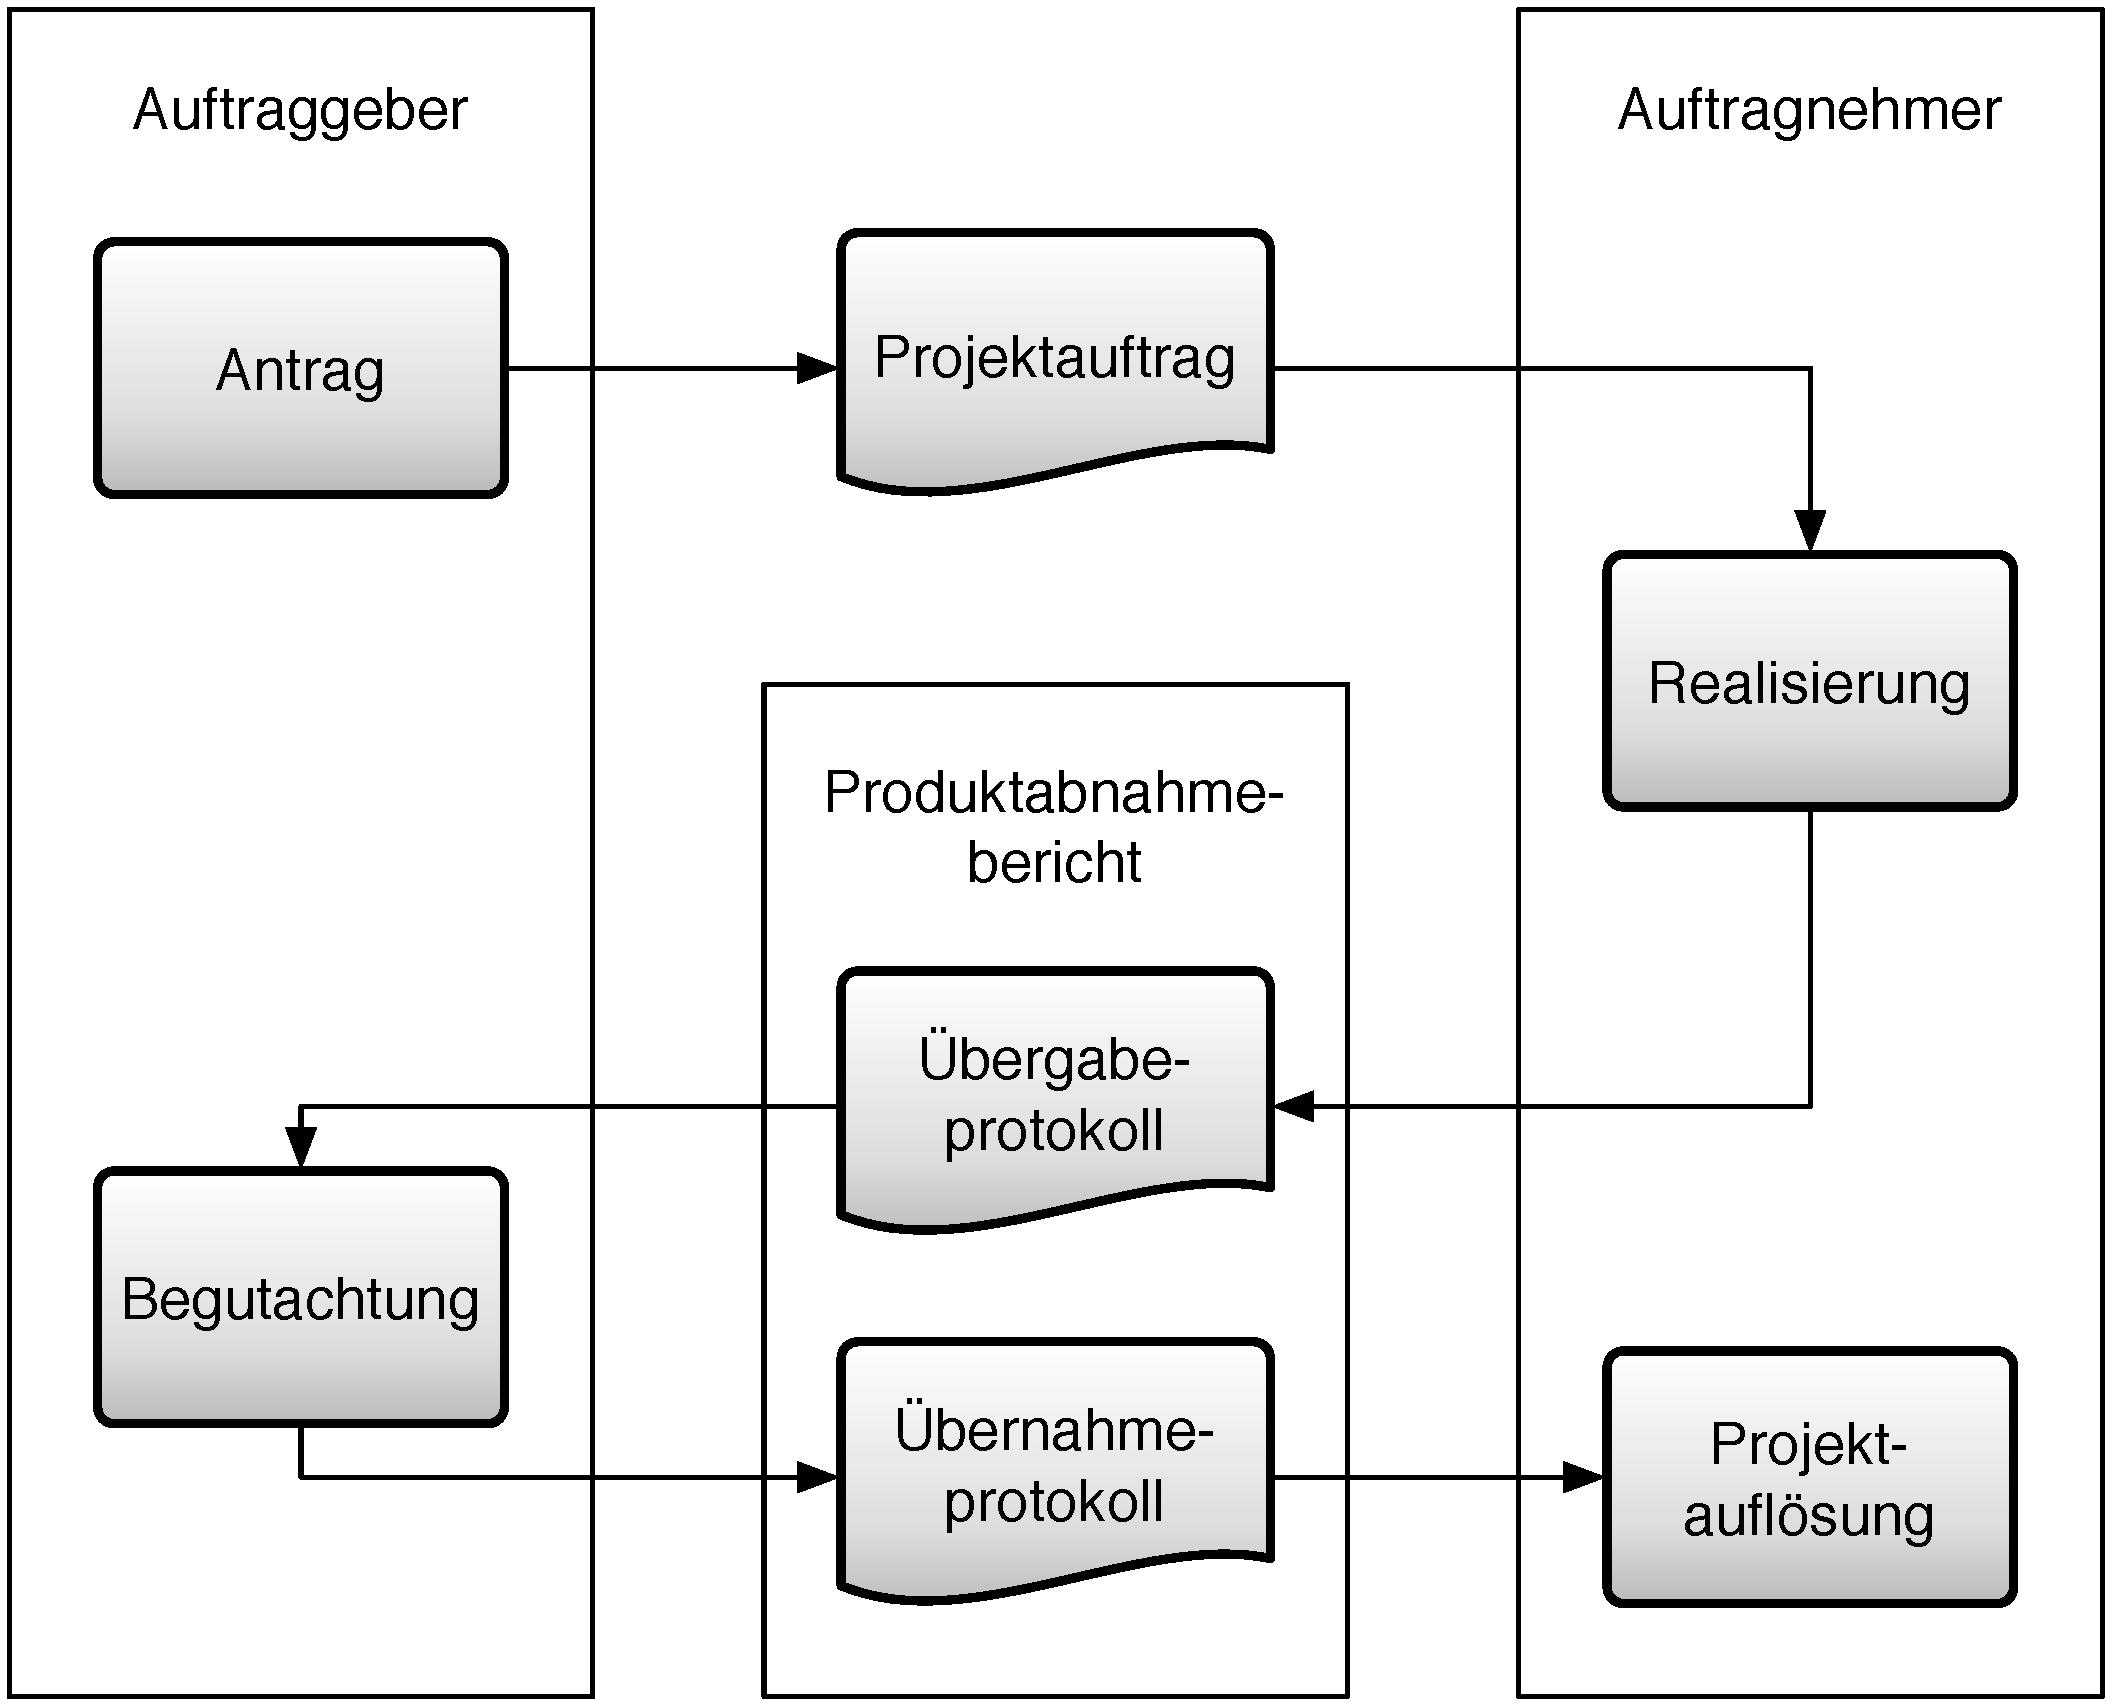
\includegraphics[width=0.6\textwidth,angle=0]{./bilder/theorie/07_produkteuebergabe.pdf}
\caption[Produkteabnahmebericht in der Produktübergabe]{Produkteabnahmebericht in der Produktübergabe\footnotemark}
\label{pic:07_produkteuebergabe}
\end{center}
\end{figure}
\footnotetext{Eigene Darstellung des Schemas in Anlehnung an \citealp*[Bild 5.2]{burghardt2007einfuehrung}}

Der Produktabnahmebericht sollte eine Beschreibung der Ergebnisse und eventuelle
Nachforderungen beinhalten. In der Regel beginnt nach der Abnahme die
Gewährleistungsfrist. Das bedeutet, dass der Zeitpunkt der Produktabnahme von
rechtlicher Relevanz sein kann und der Produktabnahmebericht vom Auftraggeber
unterschrieben werden sollte.\footnote{\citealp*[Vgl.][S. 86]{cronenbroeck2004handbuch}}

In der Projektabschlussanalyse wird die erstellte Wirtschaftlichkeitsrechnung
auf ihre Einhaltung durchleuchtet. Zusätzlich werden die Einhaltung der Termine sowie
Leistungs- und Qualitätsmerkmale betrachtet. Wichtige Kennzahlen sind zudem
die Änderungshäufigkeit und Fehlerquote.\footnote{\citealp*[Vgl.][S. 265]{schelle2007projekte}}
Grundsätzlich sollten alle gesammelten Daten in eine Art Erfahrungsdatenbank 
des Unternehmens einfliessen. Diese Daten stellen eine wichtige Voraussetzung für das 
Optimieren von Aufwandsschätzungen dar und können somit auf zukünftige Projekte 
eine positive Wirkung haben.\footnote{\citealp*[Vgl.][S. 275]{burghardt2007einfuehrung}}

\clearpage

\begin{figure}[htbp]
\begin{center}
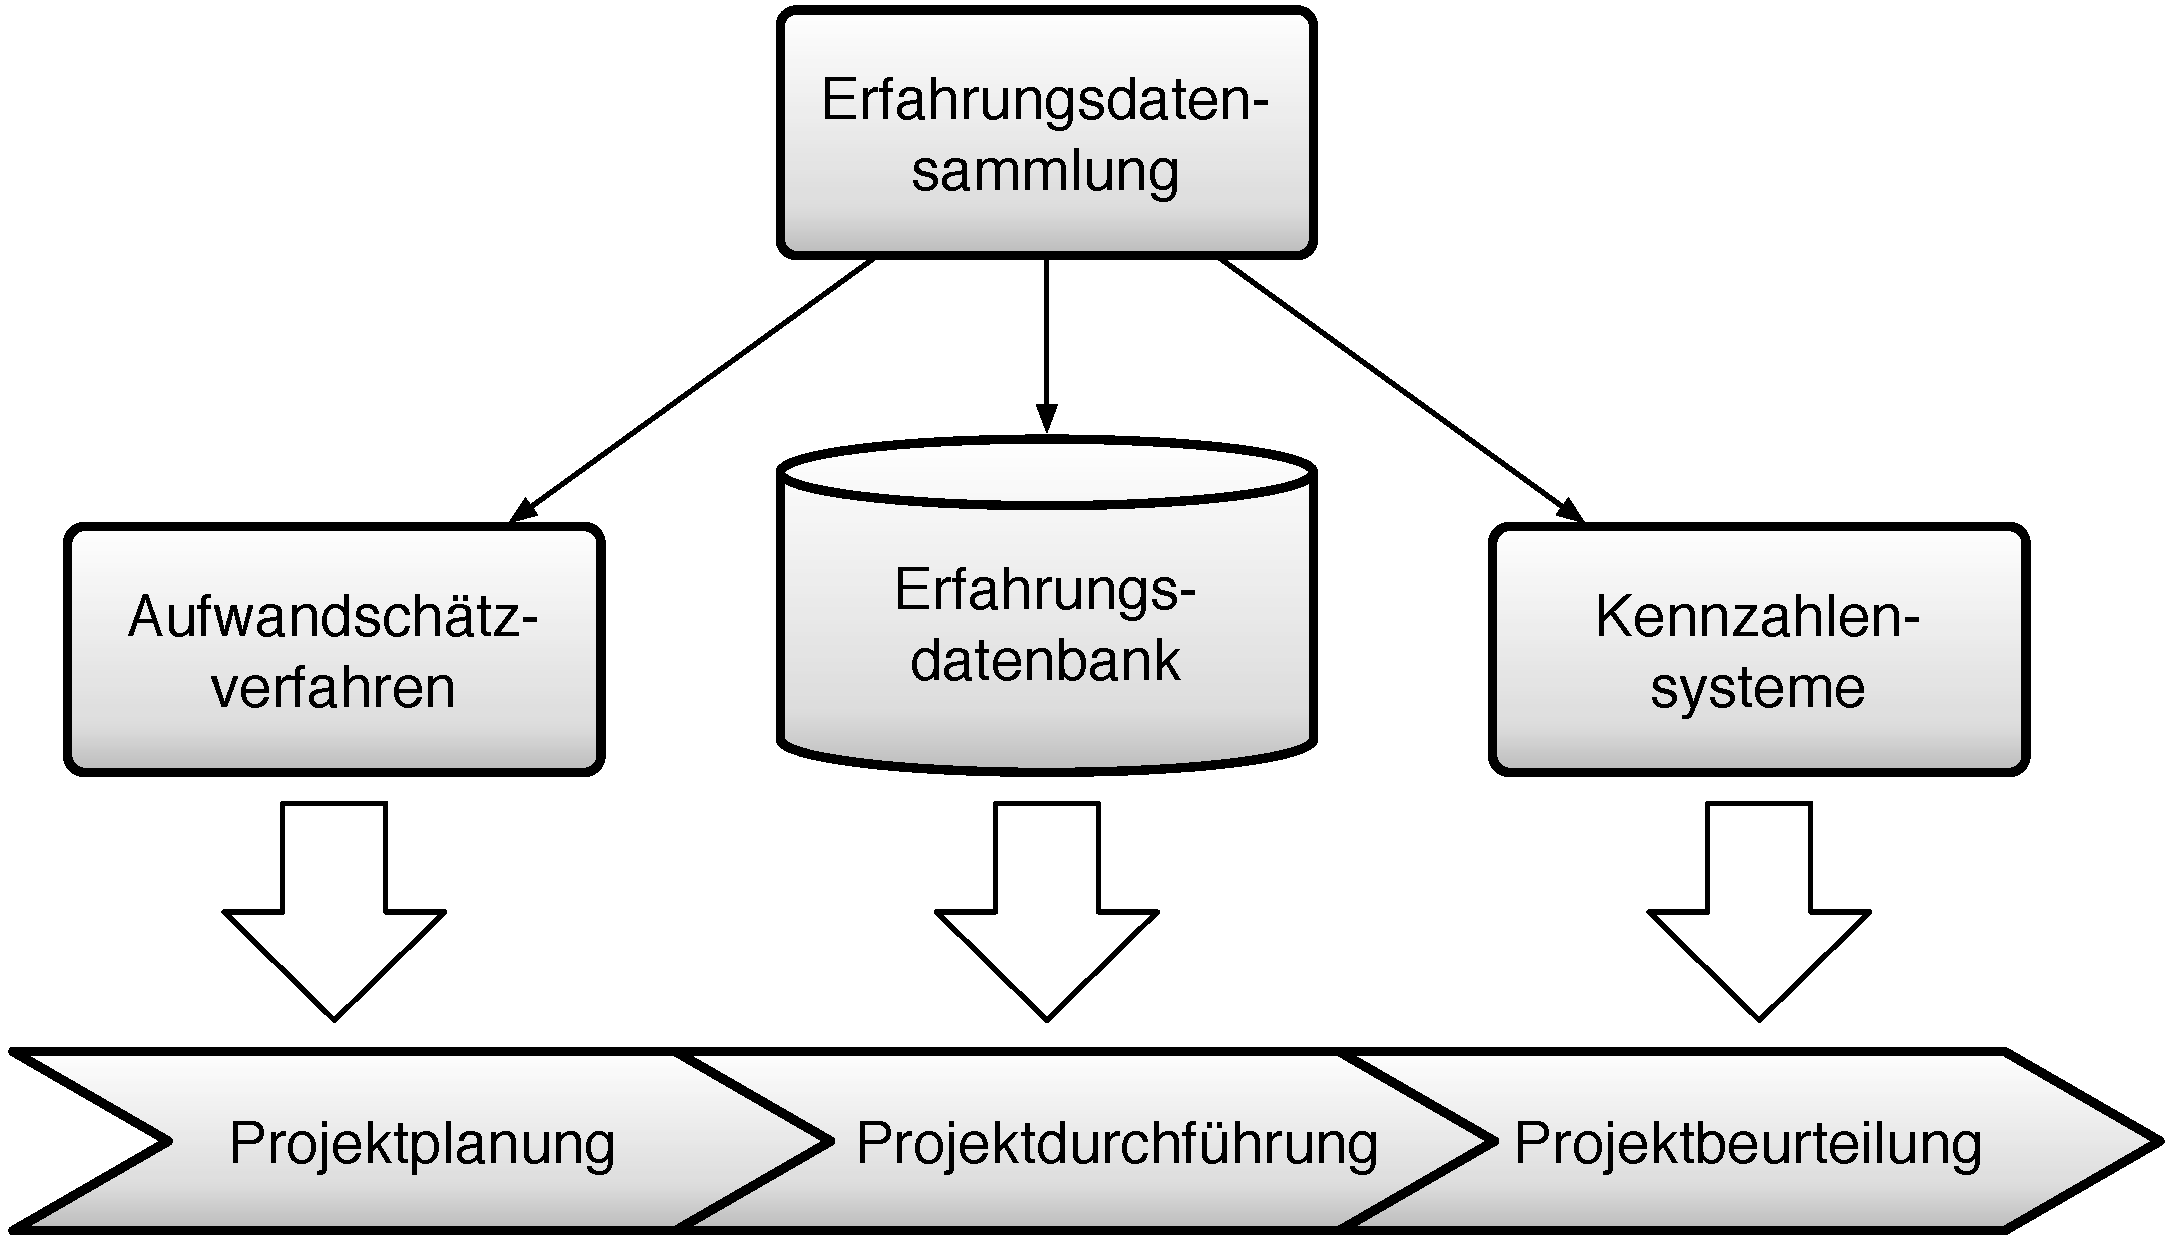
\includegraphics[width=0.6\textwidth,angle=0]{./bilder/theorie/04_unterteilung_erfahrungsdaten.pdf}
\caption[Unterteilung der Erfahrungsdaten]{Unterteilung der Erfahrungsdaten\footnotemark}
\label{pic:04_unterteilung_erfahrungsdaten}
\end{center}
\end{figure}
\footnotetext{Eigene Darstellung des Schemas in Anlehnung an \citealp*[Bild 5.7]{burghardt2007einfuehrung}}

Die Projektauflösung ist der letzte Schritt in der Projektabschlussphase. Wie 
zu Beginn erwähnt soll jedes Projekt auch ein eindeutiges Ende haben. Dies ist
für die Projektmitarbeiter besonders wichtig, da sie dann offiziell von dem
Projekt entbunden sind und in neue Projekte und Aufgaben übergeleitet werden
können. Möglicherweise ist es je nach Projekt auch sinnvoll, einen Abschluss
gebührend zu feiern.

\section{Zwischenfazit}
Die Theoretischen Grundlagen des Projektmanagements bieten einen guten Raster
mit genügend Flexibilität um einen Projektablauf auf verschieden Arten umzusetzen.
Es wird nun in der Analyse des bestehenden Projektablaufes im Kapitel \ref{chap:analyse}
darauf geachtet, welche Bereiche dieser Grundlagen bereits tangiert, umgesetzt
oder gar ganz ignoriert werden. An diesen Stellen wird jeweils auf die Theorie
verwiesen.

Bei der Aufnahme der Bedürfnisse und Anforderungen im Kapitel \ref{chap:anforderungen} 
wird darauf geachtet, welche Veränderungen bestrebt werden müssen um die in 
der Theorie empfohlenen Methoden und Hilfsmittel besser umsetzen zu können.
Beim zu erarbeitenden Lösungsansatz im Kapitel \ref{chap:loesungsansatz} wird dann versucht, 
das neue Projektmanagement und den neuen Projektablauf stärker an die Theorie 
anzulehnen.
  
  \chapter{Analyse}\label{chap:analyse}
  \section{Unternehmen}
Die allink GmbH wurde 2005 von den drei Partner David Zangger, Christoph Schlatter
und Michael Walder gegründet. David Zangger und Christoph Schlatter kümmern sich
seit jeher als Creative Directors um die grafischen Umsetzungen und die Designqualität.
Michael Walder kümmerte sich bis 2010 nebst den geschäftsführerischen Tätigkeiten
auch um die ganze Informatik. Nach der Fusionierung mit der SiSprocom übergab
er die Leitung der Informatik an Silvan Spross ab und widmet sich nun dem Aufbau der
Beratung und Projektleitung. Seit 2010 bezeichnet sich allink als die interdisziplinäre 
und marktnahe Designagentur, wie man ihrer Website entnehmen kann:

\begin{quote}
``allink.creative ist eine Designagentur, die Produkte, Marken und Unternehmen 
attraktiv und einzigartig in Szene setzt. Unser Design soll Menschen erreichen 
und begeistern. Weil wir marktnah arbeiten, stellen wir den wirtschaftlichen 
Nutzen von Design stets in den Vordergrund.

Wir arbeiten interdisziplinär, damit wir die breiten Möglichkeiten an 
Kommunikationskanälen optimal für unsere Kunden einsetzen können. Unser 
Team von Spezialisten aus den vielfältigsten Bereichen findet innovative 
und gesamtheitliche Lösungen, um Marken und Firmen wirkungsvoll zu positionieren. 
Die Bereiche Branding, Online Communication, Packaging Design und Product 
Design zählen dabei zu unseren Kernkompetenzen.''
\end{quote}

Das Unternehmen lässt sich zur Zeit in die drei Hauptbereiche Beratung, Grafik
und Informatik unterteilen.

\begin{figure}[htbp]
\begin{center}
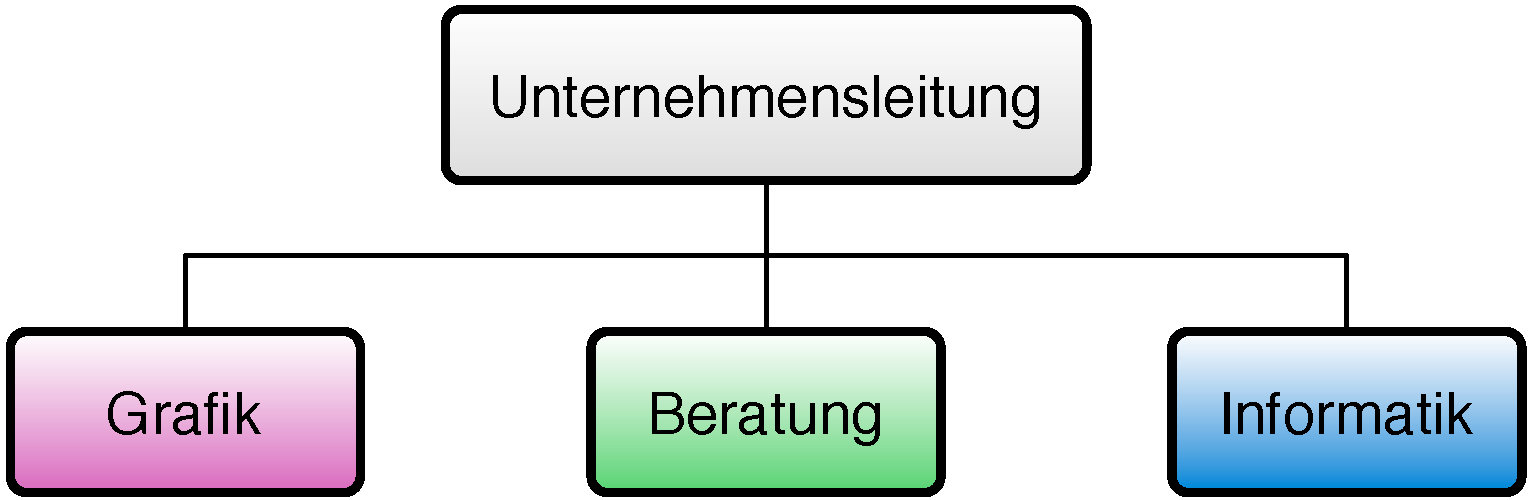
\includegraphics[width=0.46\textwidth,angle=0]{./bilder/analyse/04_funktionales_organigramm.pdf}
\caption{Funktionales Organigramm von allink}
\label{pic:04_funktionales_organigramm}
\end{center}
\end{figure}

Wobei sich jeweils ein bis zwei Partner um einen
Bereich kümmern. Dies beinhaltet nebst den Alltagsarbeiten auch organisatorische 
Aufgaben wie das Personalmanagement und die Verteilung der Arbeitspakete an den 
geeignetsten Mitarbeiter. In der Grafik \ref{pic:mitarbeiter_pro_bereich} 
sind die Mitarbeiter pro Bereich abgebildet.

\begin{figure}[htbp]
\begin{center}
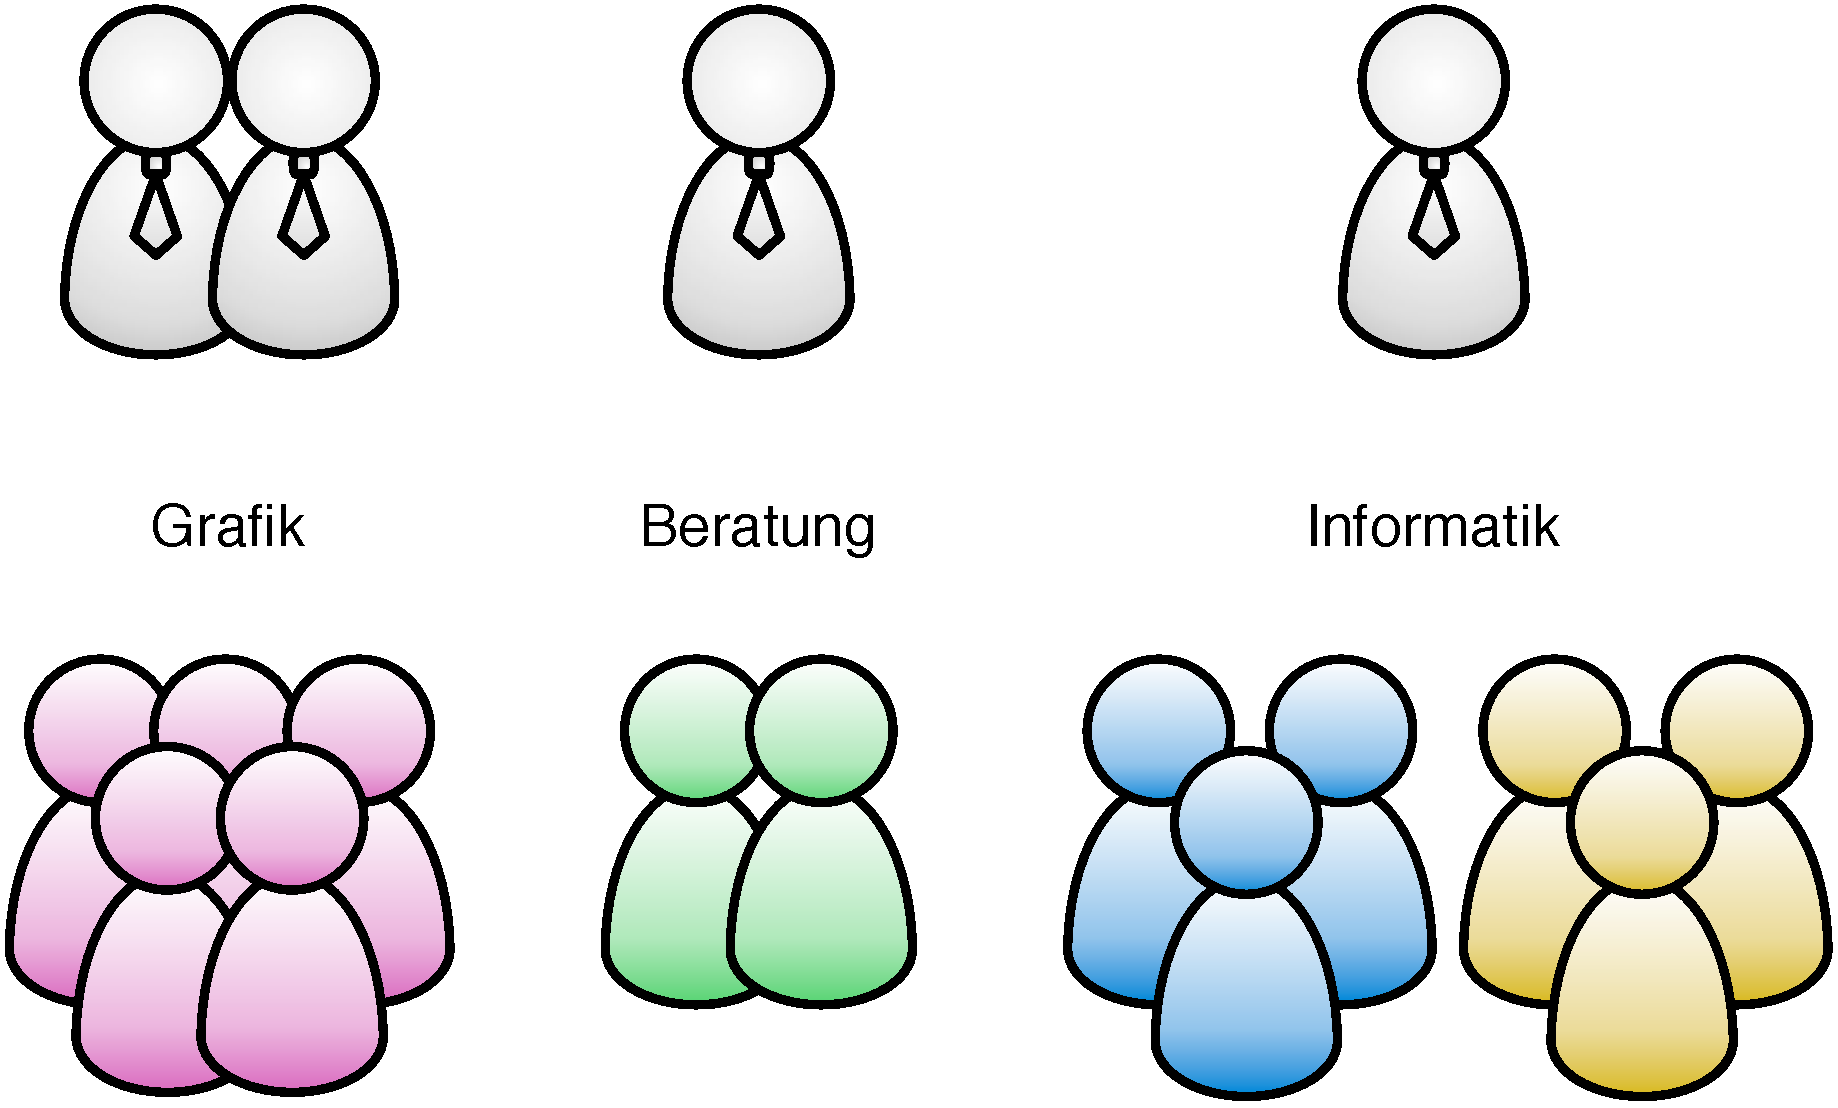
\includegraphics[width=0.55\textwidth,angle=0]{./bilder/analyse/mitarbeiter_pro_bereich.pdf}
\caption{Übersicht der Mitarbeitern pro Bereich}
\label{pic:mitarbeiter_pro_bereich}
\end{center}
\end{figure}

Im Bereich Grafik sind nebst drei Vollzeitangestellen noch ein Praktikant und eine
Lehrtochter angestellt. In der Beratung beschäftigt allink zur Zeit zwei Mitarbeiter.
Die Informatik setzt sich aus zwei Vollzeitangestellten sowie einem Pratikant
zusammen. Die drei weiteren Informatiker arbeiten als externe Berater und
werden höchst selten in einem internen Projekt beschäftigt.

Trotz dieser Aufteilung in mehrere Bereiche geht der Kommunikationsweg nicht
immer über die für den Mitarbeiter zuständigen Partner. 

\begin{figure}[htbp]
\begin{center}
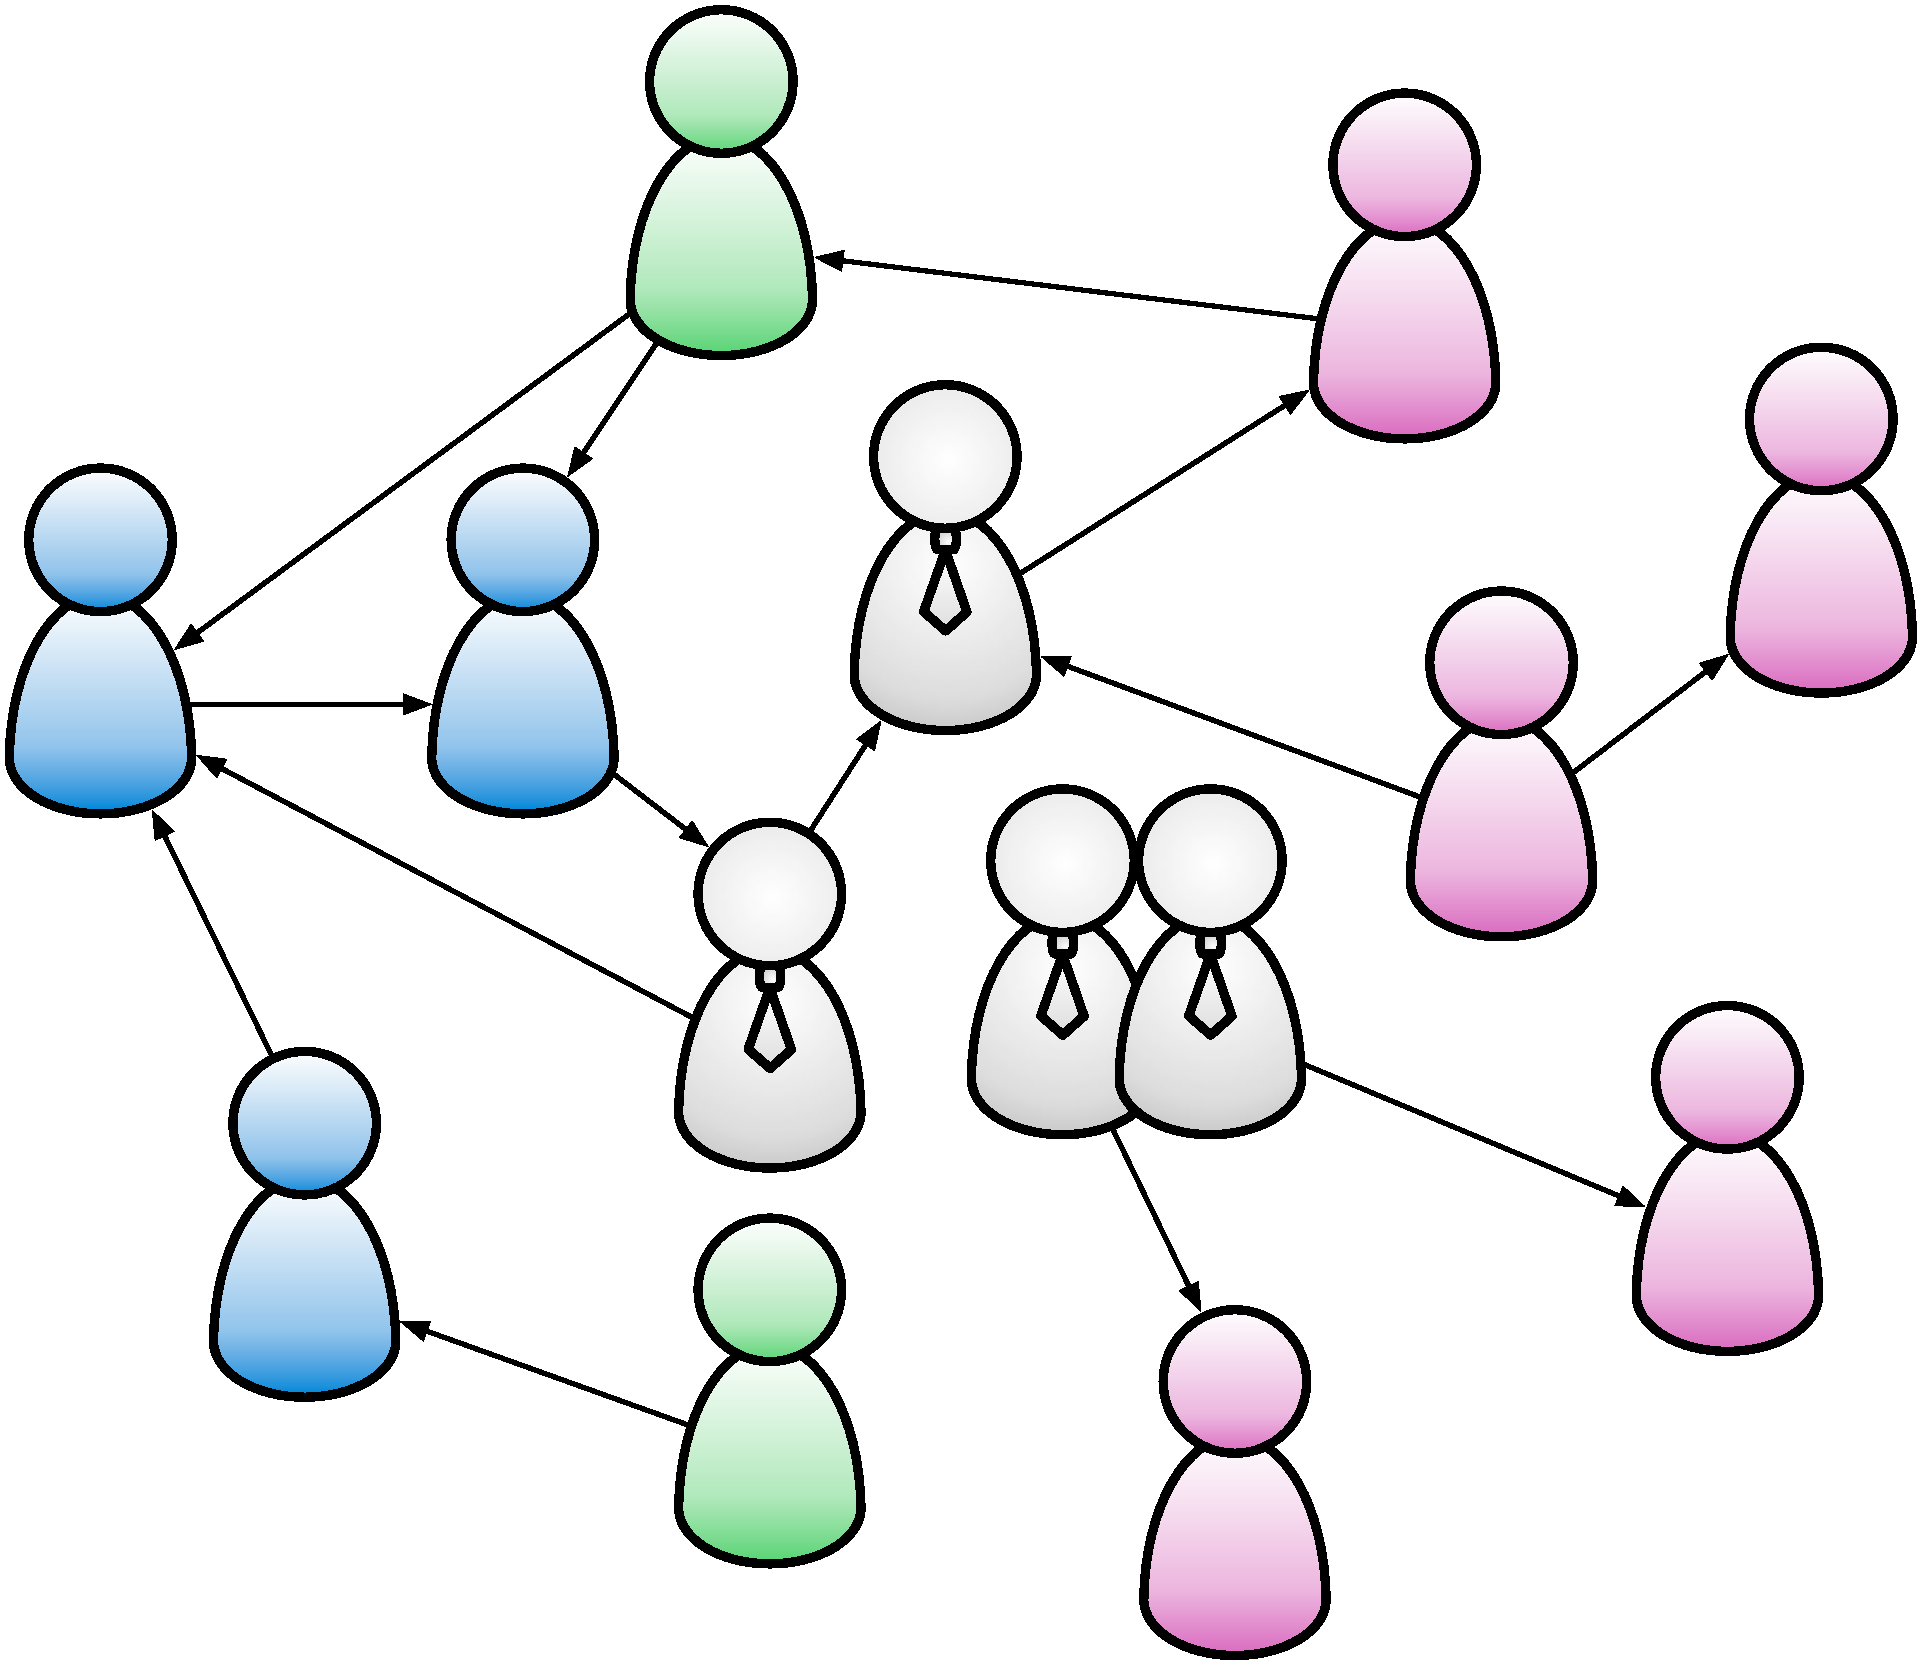
\includegraphics[width=0.40\textwidth,angle=0]{./bilder/analyse/kommunikationswege.pdf}
\caption{Beispiel der unorganisierten Kommunikationswege}
\label{pic:kommunikationswege}
\end{center}
\end{figure}

Das ist auch grundsätzlich nicht zu vermeiden, bzw. das muss zu einem gewissen
Grad auch der Fall sein. Ansonsten wären die Abläufe von wenigen Anlaufstellen abhängig
und das ganze würde ins Stocken geraten. Trotzdem birgt es gewisse Schwachstellen.
Zum Beispiel, dass nicht alle Beteiligten eines Projektes den gleichen Informationsstand 
haben. Dies kann sich beim Kontakt mit einem Kunden negativ auswirken, wenn der
Kunde schon über etwas in Kenntnis gesetzt wurde, und der Mitarbeiter am
Telefon selbst gar noch über die selben Informationen verfügt. Die Schwächen 
werden in der Analyse des Projektablaufes noch genauer beleuchtet.

Der Aufbau einer Beratung, die zur Zeit im Gange ist, soll genau solche Probleme
lösen. Jedoch steckt allink hier noch in den Kinderschuhen und erhofft sich
unteranderem aus dieser Arbeit Erkenntnisse über einen möglichst optimalen 
Projektablauf.


\section{Kunden}
Im Gegensatz zur SiSprocom hat die allink einen relativ grossen Kundenstamm.
Das bedeutet, dass kein grosses Klumpenrisiko existiert. Jedoch ist auch
die Auftragskontinuität der einzelnen Kunden viel kleiner. Für manche arbeitet
allink jeden Monat an einem neuen Projekt, für anderen einmal im Jahr.
In der Grafik \ref{pic:kundenauszug} ist ein Teil der Kunden abgebildet.

\begin{figure}[htbp]
\begin{center}

\includegraphics[width=0.8\textwidth,angle=0]{./bilder/analyse/kundenauszug.jpg}
\caption{Kundenauszug von allink}
\label{pic:kundenauszug}
\end{center}
\end{figure}

Unterteilt man die Kunden von allink in die gängigen Firmengrössen Kleinstunternehmen,
kleine Unternehmen und mittlere Unternehmen, so gelangt man zu einer interessanten 
Verteilung. Die Definition der Unternehmensgrössen basiert auf einer Empfehlung
der Kommission der Europäischen Union\footnote{\citealp*[Vgl.][Anhang Art. 2]{eu_komission_unternehmen}}.
Diese unterteilt die Unternehmen nach dem in der Tabelle \ref{tab:eu_unterteilung} 
abgebildetem Schlüssel.

\begin{table}[h]
\begin{center}
    \begin{tabular}{clccccc}
        \toprule \textbf{Typ} & \textbf{Beschäftigte} & & \textbf{Umsatzerlös} & & \textbf{Bilanzsumme} \\
        \midrule Kleinstunternehmen & $<$ 10 & und & $\leq$ 2 Mio \euro & oder & $\leq$ 2 Mio \euro \\
        \midrule Kleine Unternehmen & $<$ 50 & und & $\leq$ 10 Mio \euro & oder & $\leq$ 10 Mio \euro \\
        \midrule Mittlere Unternehmen & $<$ 250 & und & $\leq$ 50 Mio \euro & oder & $\leq$ 43 Mio \euro \\
        \bottomrule
    \end{tabular}
    \caption{Empfehlung Unternehmensunterteilung, Kommission der Europäischen Union}
    \label{tab:eu_unterteilung}
\end{center}
\end{table}

Die Kategorisierung der Kunden, abgebildet in der nachstehenden Grafik \ref{pic:kundenkategorisierung},
basiert überwiegend auf den Informationen von moneyhouse\footnote{moneyhouse bietet Handelsregister- und Firmendaten, \url{http://www.moneyhouse.ch}}, 
da man nicht alle Kunden um aktuelle Mitarbeiter- und Umsatzzahlen bitten konnte.
Zusätzlich zu den in der Tabelle \ref{tab:eu_unterteilung} aufgelisteten Kategorien 
wurde noch die Kategorie ``Grosse Unternehmen'' hinzugefügt, um Firmen mit genau 
oder mehr als 250 Mitarbeiter kategorisieren zu können.

Es wird absichtlich nicht die vollständige Liste der Kunden von allink und deren 
Kategorisierung beigelegt, da allink nicht alle Kunden in dieser Arbeit namentlich 
aufgelistet haben möchte. Bei Bedarf kann die Liste aber bei allink eingesehen werden.

\begin{figure}[htbp]
\begin{center}
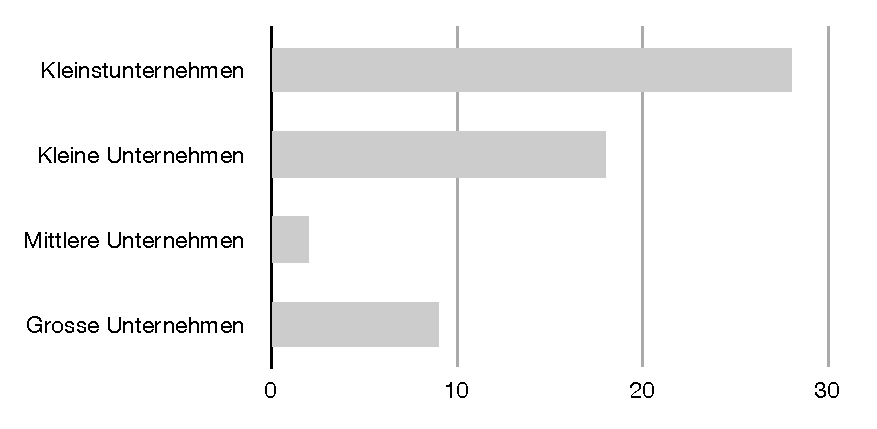
\includegraphics[width=0.75\textwidth,angle=0]{./bilder/analyse/kundenkategorisierung.pdf}
\caption{Anzahl Kunden der allink in Unternehmensgrössen kategorisiert}
\label{pic:kundenkategorisierung}
\end{center}
\end{figure}

Wie man erkennen kann, arbeitet allink überwiegend mit Kleinst- und kleinen 
Unternehmungen zusammen. Interessanterweise aber mehr grosse als mittlere
Unternehmen. Die verschiedenen Firmenkulturen der Kunden haben auch einen 
Einfluss auf die Projektabläufe. Grundsätzlich stellen sich wohl alle Kunden
der Herausforderung, ihre Projekte gut zu organisieren. Je nach Auflagen oder
Abläufe der Kunden, hat dies auch Auswirkungen auf den Projektablauf der allink.
Deshalb wäre es falsch anzunehmen, dass sie zur Zeit bei jedem Projekt und 
Kunden das selbe Vorgehen anwenden können.

Möglicherweise genau deshalb existiert zur Zeit kein definierter Projektablauf. 
Doch gibt es klar erkennbare Gemeinsamkeiten über alle Projekte, bzw. Projektabläufe.
Im nächsten Kapitel \ref{chap:projektablauf} wird versucht, den heutigen Projektablauf so 
abzubilden, dass er für die meisten vergangenen Projekte Gültigkeit hat.


\section{Projektablauf}\label{chap:projektablauf}
Den heutigen Projektablauf bei der allink könnte man am Besten als ``natürliches Vorgehen''
umschreiben. Ein potentielles Projekt kommt an einen Partner heran, entweder über 
eine Anfrage oder eine Akquisition, der spricht sich mit den anderen Partner ab 
und nimmt dann die Mitarbeiter mit in das Projekt, die er als nötig erachtet.
Dies kommt einem Projektmanamgement organisiert über die Linie aus der Theorie
am nächsten.

Der Projektablauf wird in drei Prozesse, die Projektannahme und Offertenerstellung,
die Projektdurchführung und der Projektabschluss unterteilt und dazu die 
Ablaufdiagramme erstellt. Darin wird jede Aktion mit einer eindeutigen Nummer versehen,
um danach darauf im beschreibenden Text verweisen zu können. Nach einer Entscheidung erhöht
sich die Laufnummer jeweils um eine ganze Zahl, um die verschiedenen Wege hervorzuheben.
Zusätzlich werden die Abläufe um die Tools, die verwendet werden, ergänzt.
Es werden nicht immer alle erwähnten Tools in dem selben Projekt eingesetzt,
jedoch Projektübergreifend betrachtet, kommen alle mal beim zugeordneten Schritt 
zum Einsatz. Die verwendete Software wird zu einem späteren Zeitpunkt separat
behandelt, da es zu diesem Zeitpunkt das ``Wie?'' und nicht ``Womit?'' betrachtet
wird.

\clearpage

\subsection{Projektannahme und Offertenerstellung}

\begin{figure}[p]
\begin{center}
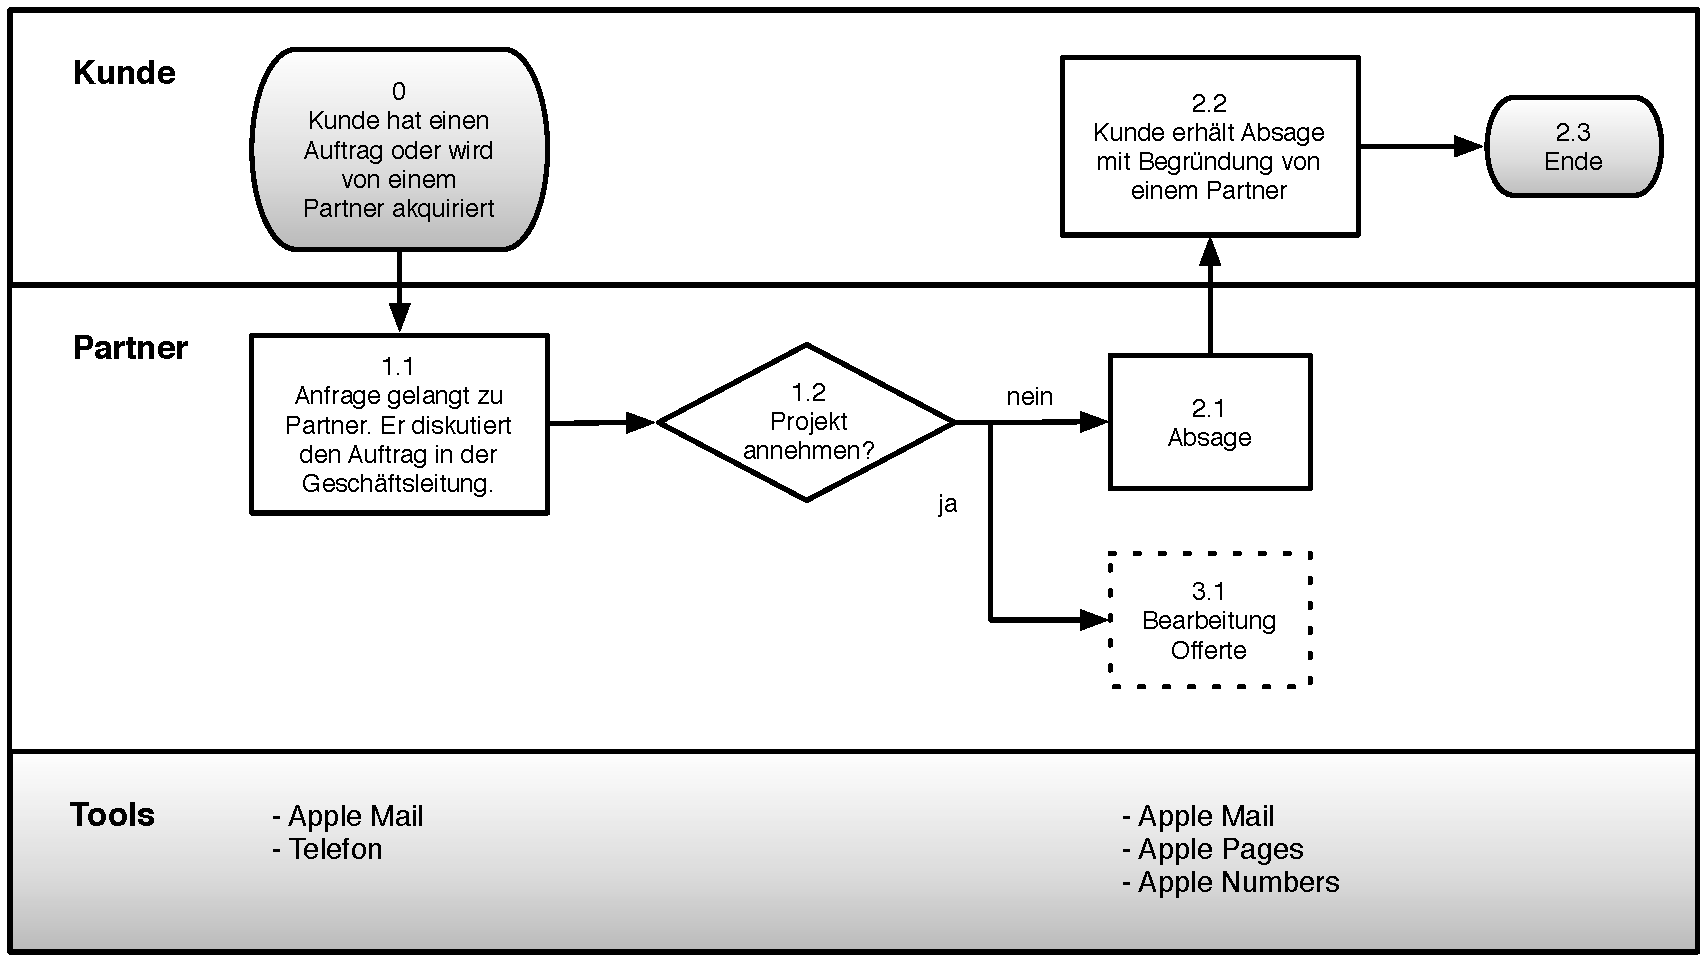
\includegraphics[width=0.99\textwidth,angle=0]{./bilder/analyse/01_ist_prozesse_offerte_01.pdf}
\caption[Offertenerstellungs Prozess von allink 1/2]{Offertenerstellungs 
    Prozess von allink 1/2\footnotemark}
\label{pic:01_ist_prozesse_offerte_01}
\end{center}
\end{figure}
\footnotetext{Eigene Darstellung}

\begin{figure}[p]
\begin{center}
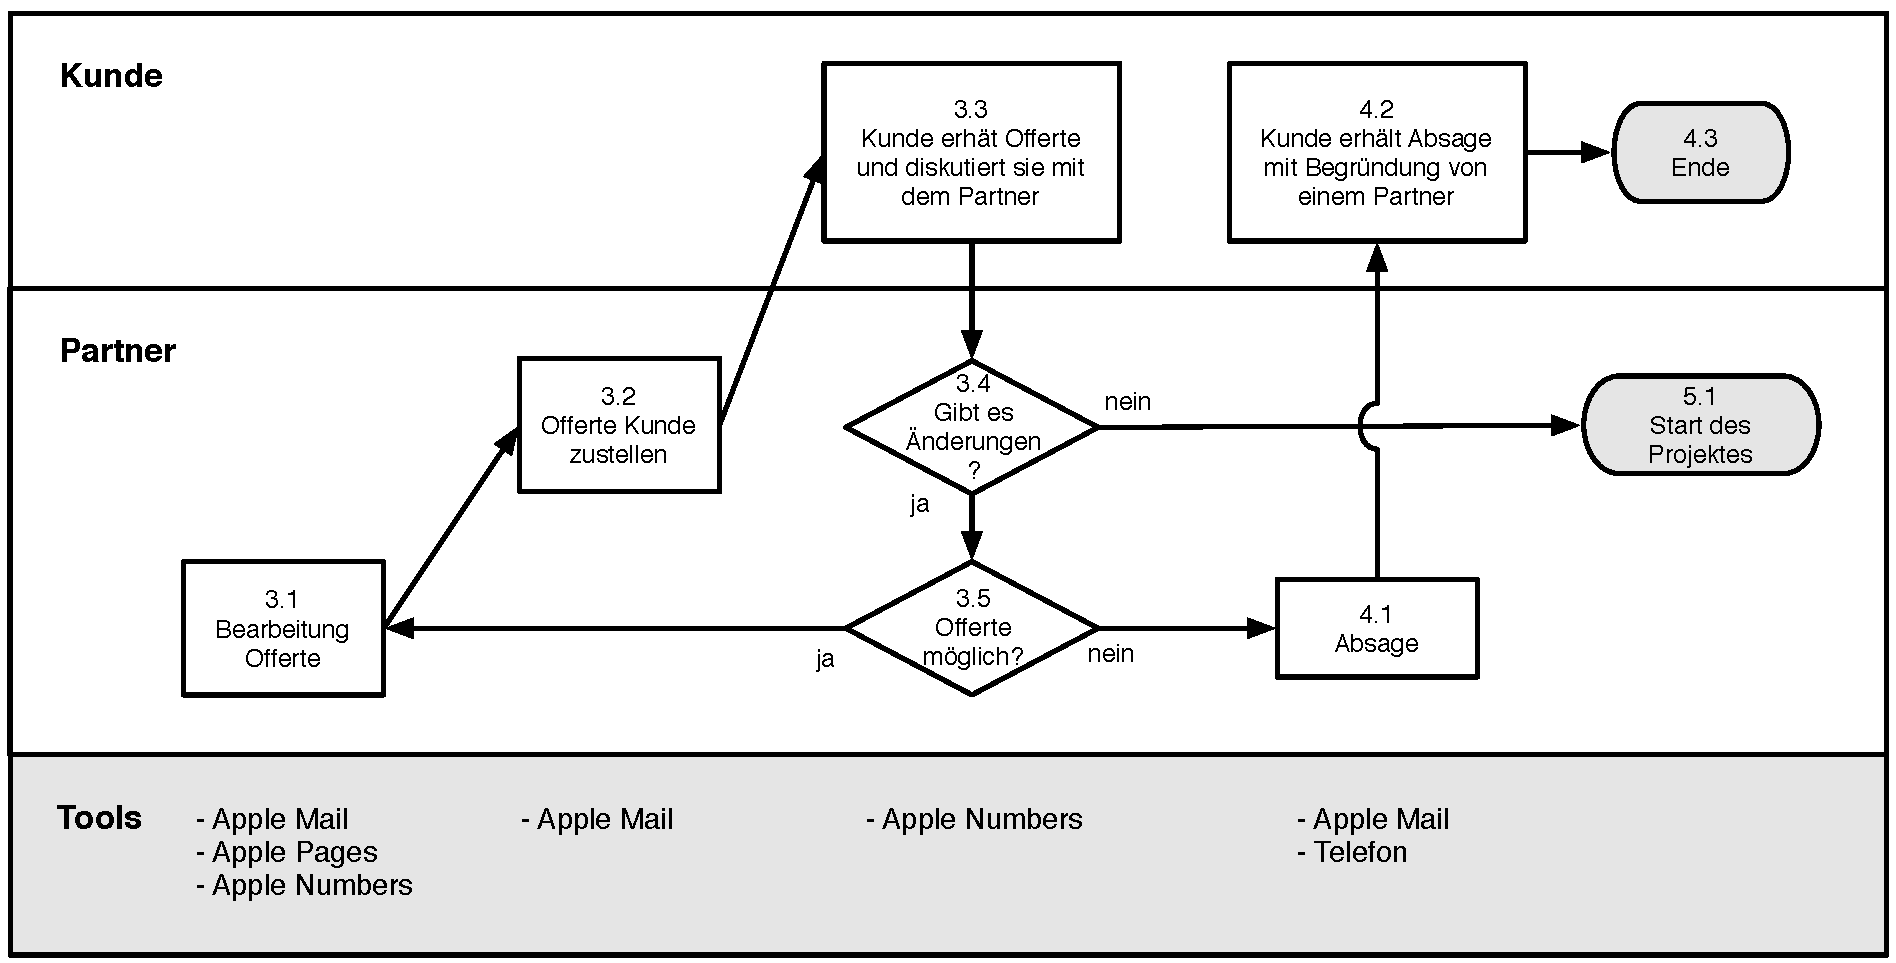
\includegraphics[width=0.99\textwidth,angle=0]{./bilder/analyse/01_ist_prozesse_offerte_02.pdf}
\caption[Offertenerstellungs Prozess von allink 2/2]{Offertenerstellungs 
    Prozess von allink 2/2\footnotemark}
\label{pic:01_ist_prozesse_offerte_02}
\end{center}
\end{figure}
\footnotetext{Eigene Darstellung}

In den Darstellungen \ref{pic:01_ist_prozesse_offerte_01} und
\ref{pic:01_ist_prozesse_offerte_02} ist der aktuelle Prozess der Offertenerstellung 
ersichtlich. Die darin verwickelten Akteuere sind der Kunde und der bzw. die Partner.
Hier werden aus der Theorie Teile der Projektdefinition und Projektplanung abgedeckt.
Eine Projektanfrage endet entweder in einer Absage oder einem Start eines neuen 
Projektes. Wenn das Projekt nicht zustande kommt, werden zurzeit die Aufwände der
Akquisition und der Offertenerstellung vernachlässigt und somit von
den durchgeführten Projekten getragen.

Als Start eines Projektablaufes wird entweder ein neues Projekt akquiriert, 
durch eine direkte Anfrage an ein Unternehmen oder einen Pitch\footnote{Als Pitch 
wird der Wettbewerb zwischen verschiedenen Agenturen um einen Auftrag eines 
Unternehmens bezeichnet.}, oder eine Anfrage kommt direkt von einem Kunden (\textbf{0}). 
Die Projekte gelangen zum heutigen Zeitpunkt immer als erstes zu einem Partner. 
Sehr selten bringt ein Mitarbeiter durch einen seiner Kontakte ein Projekt ein. 
Aber auch in diesem Fall, würde es als erstes an einen Partner herangetragen.
Dieser diskutiert den möglichen Auftrag mit den anderen Partnern in der 
Geschäftsleitung (\textbf{1.1}). Diese entscheide demokratisch ob ein Projekt 
angenommen oder abgelehnt wird (\textbf{1.2}). Sofern nicht alle Partner anwesend 
sein können, haben die anderen Partner die Kompetenz, alleine zu entscheiden.

Im Falle einer Absage (\textbf{2.1}) tritt ein Partner wieder mit dem Kunden in Kontakt.
In den meisten Fällen natürlich der Partner, der bereits mit dem Kunden Kontakt
hatte. Dem Kunden wird erklärt, aus welchen Gründen das Projekt nicht angenommen
und durchgeführt werden kann (\textbf{2.2}).

Sollte das Projekt angenommen werden, wird auf Grund den zu erbringenden
Dienstleistungen eine möglichst genaue Offerte erstellt (\textbf{3.1}). Diese Schätzungen
basieren überwiegend auf Erfahrungswerten aus anderen Projekten. Dieses Verfahren
wird in der Theorie ebenfalls empfohlen. Es wäre jedoch sinnvoll öfters auch
die Erfahrungen von Experten zum Thema heranzuziehen. 
Die Offerte wird dann dem Kunden zugestellt (\textbf{3.2}). In vielen Fällen wird dem Kunden
die Offerte präsentiert und genauer erklärt.
Der Kunde diskutiert dann mit dem oder den Partnern die Offerte (\textbf{3.3}) und bringt
bei bedarf Änderungen und Wünsche an.
Kann man sich mit dem Kunden nicht einigen, also wünscht der Kunde Änderungen
an der Offerte oder den zu erbringenden Dienstleistungen (\textbf{3.4}), die von unserer Seite
nicht mehr möglich sind (\textbf{3.5}), muss das Projekt abgesagt werden (\textbf{4.1}).
Dem Kunden wird erklärt, aus welchen Gründen die Offerte nicht angepasst oder
die Dienstleistung nicht erbracht werden kann (\textbf{4.2}).

Im Falle einer Einigung und einer Auftragserteilung startet das eigentliche
Projekt (\textbf{5.1}).

\clearpage

\subsection{Projektdurchführung}

\begin{figure}[p]
\begin{center}
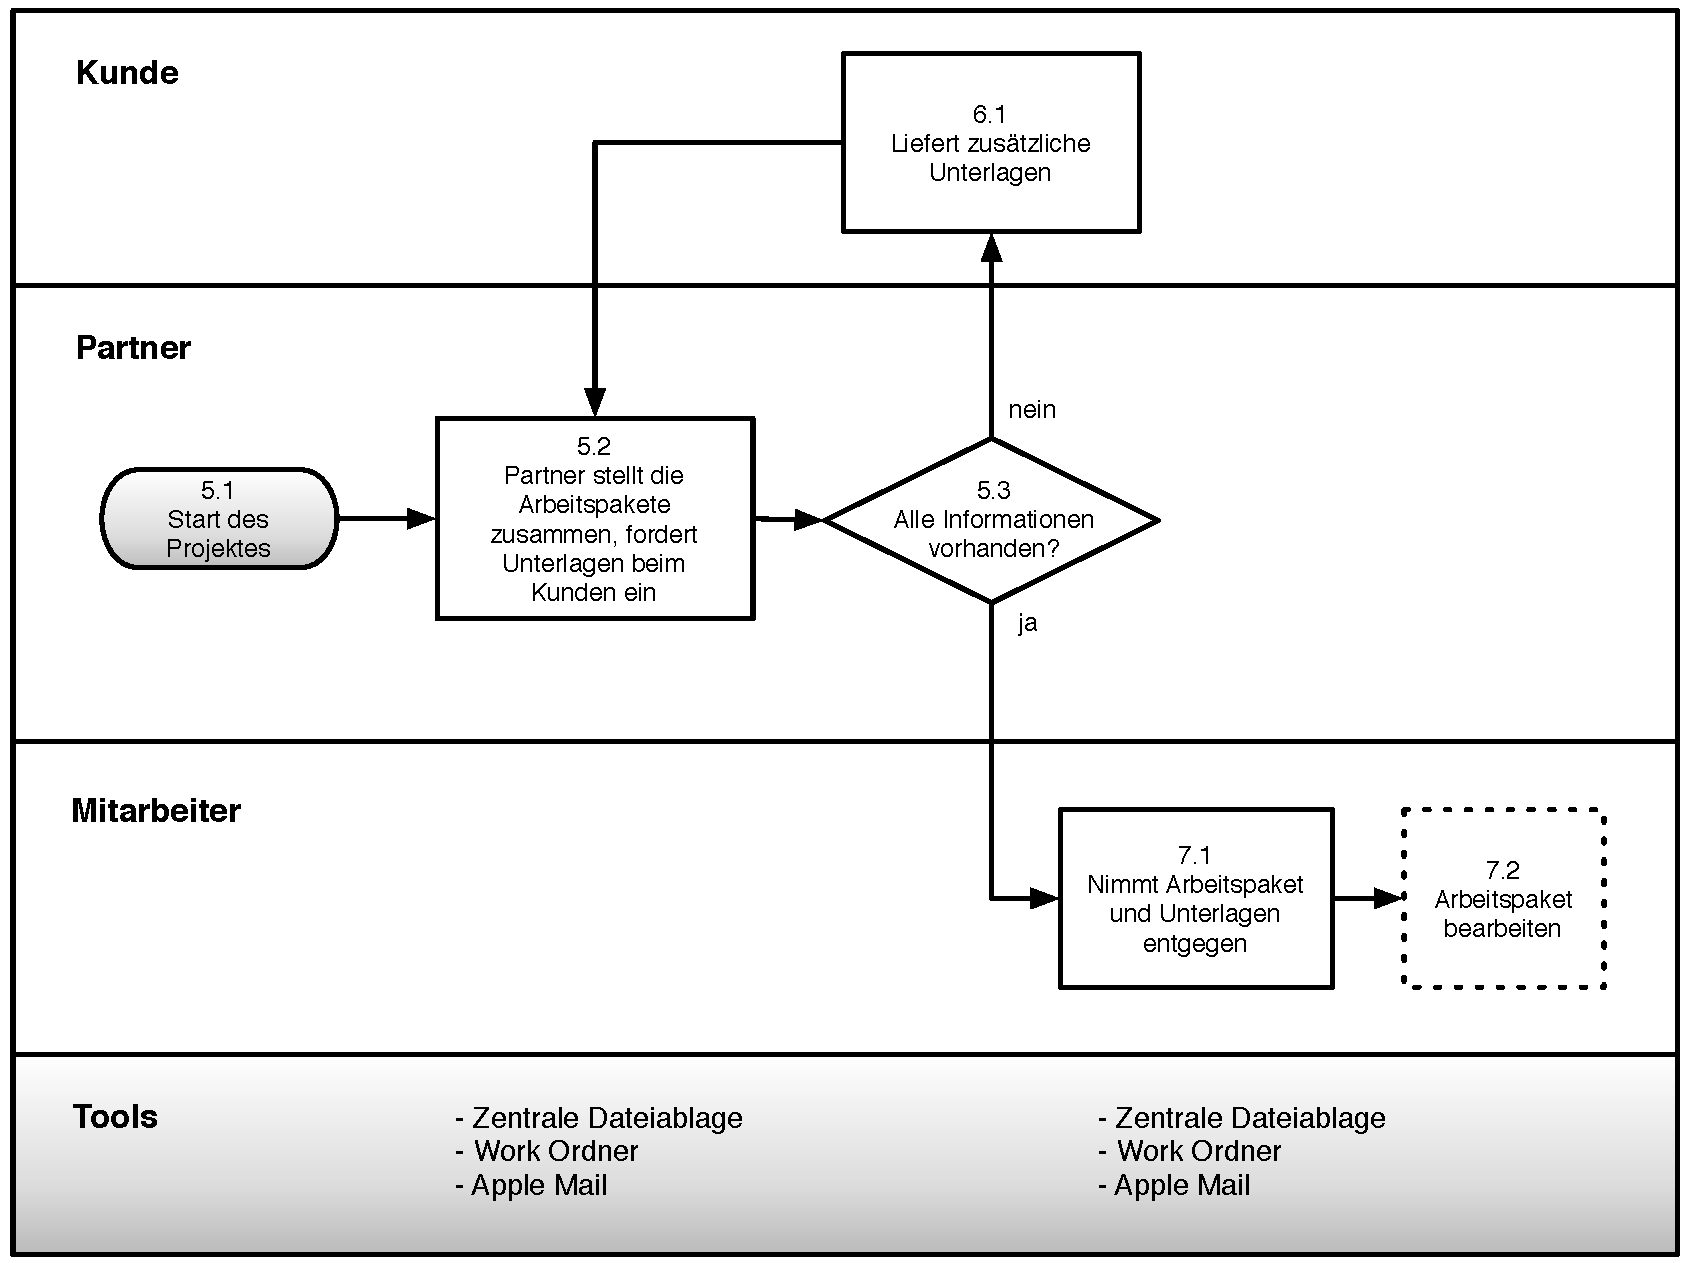
\includegraphics[width=0.99\textwidth,angle=0]{./bilder/analyse/02_ist_prozesse_arbeit_01.pdf}
\caption[Projektumsetzungs Prozess von allink 1/2]{Projektumsetzungs 
    Prozess von allink 1/2\footnotemark}
\label{pic:02_ist_prozesse_arbeit_01}
\end{center}
\end{figure}
\footnotetext{Eigene Darstellung}

\begin{figure}[p]
\begin{center}
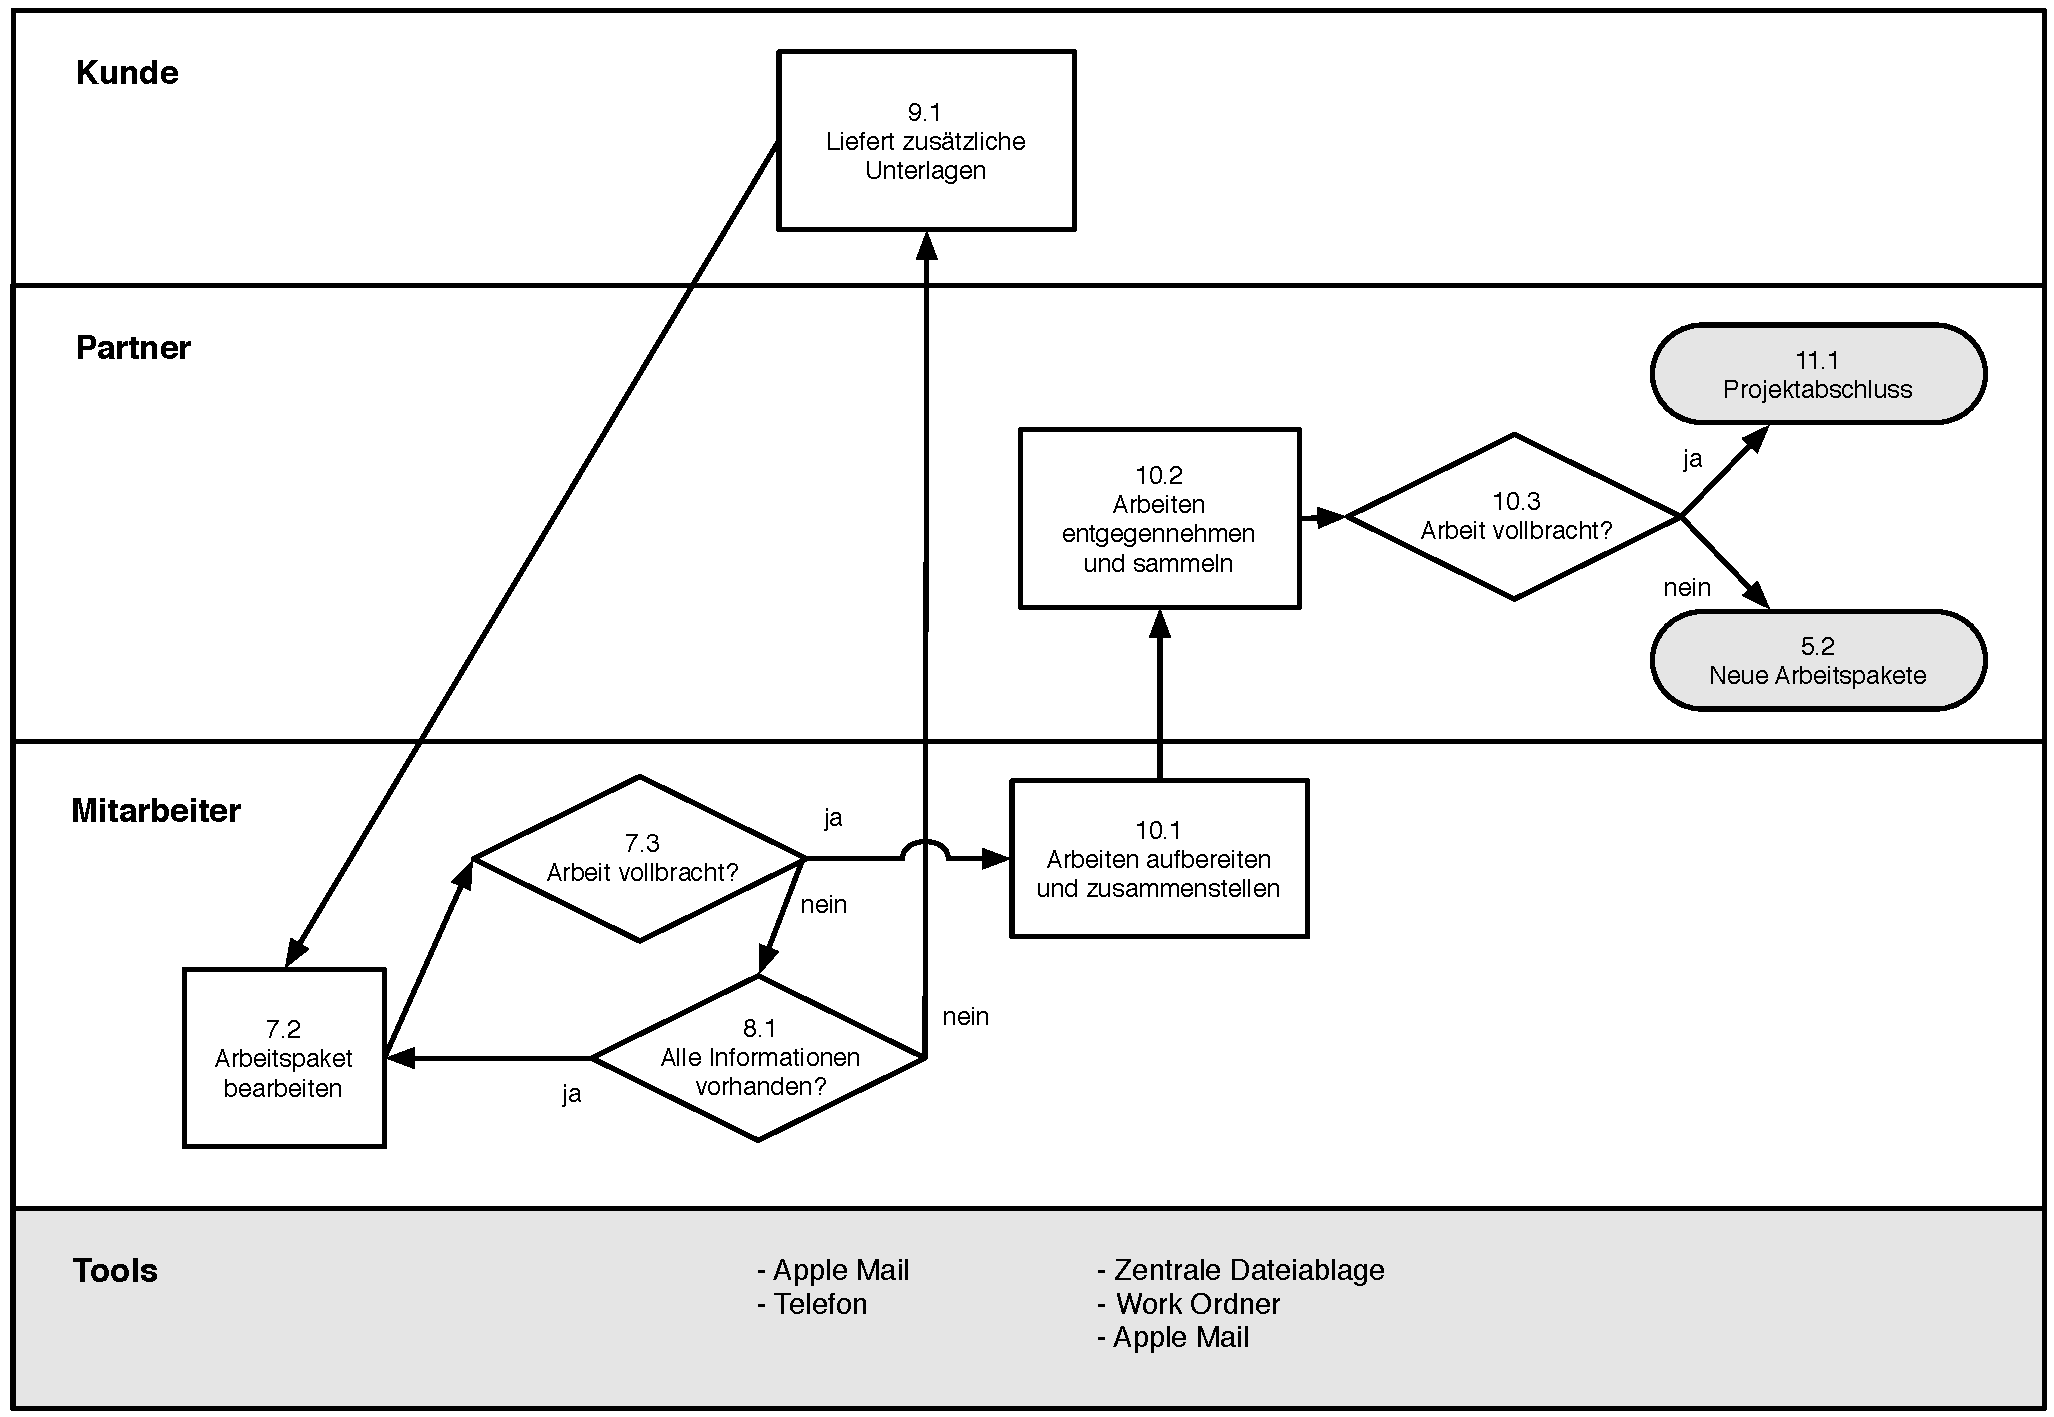
\includegraphics[width=0.99\textwidth,angle=0]{./bilder/analyse/02_ist_prozesse_arbeit_02.pdf}
\caption[Projektumsetzungs Prozess von allink 2/2]{Projektumsetzungs 
    Prozess von allink 2/2\footnotemark}
\label{pic:02_ist_prozesse_arbeit_02}
\end{center}
\end{figure}
\footnotetext{Eigene Darstellung}

In der ersten Phase der Projektdurchführung sammelt der Projektleiter bzw.
Partner alle nötigen Informationen, die zur Bearbeitung des Projektes notwendig sind.
Danach erstellt er Arbeitspakete zusammen, die er wiederum an die Mitarbeiter verteilt.
Die Projektdurchführung ist in den Grafiken \ref{pic:02_ist_prozesse_arbeit_01} und 
\ref{pic:02_ist_prozesse_arbeit_02} grafisch dargestellt.

Der Partner verschafft sich einen überblick über das Projekt und gruppiert
die zu erledigenden Arbeiten in Arbeitspakete (\textbf{5.2}). Er besorgt alle nötigen Informationen
und Unterlagen, die zur Bewältigung eines Arbeitspaketes notwendig sind und fordert
bei Kunden wenn nötig noch mehr Informationen und Unterlagen ein (\textbf{6.1}).
Sind alle Informationen vorhanden (\textbf{5.3}) übergibt er die Arbeitspakete
den Mitarbeitern zur Erledigung.

Der Mitarbeiter nimmt das Arbeitspaket entgegen (\textbf{7.1}) und beginnt
mit dessen Bearbeitung (\textbf{7.2}). Stellt sich heraus, dass er sein Arbeitspaket
noch nicht abschliessen kann (\textbf{7.3}) und noch mehr Informationen oder
Unterlagen benötigt (\textbf{8.1}), kommt es oft vor, dass der Mitarbeiter
eigenständig beim Kunden zusätzliche Unterlagen einfordert (\textbf{9.1}).
Sobald er ein Paket abschliessen kann, stellt er alles Erarbeitete zusammen (\textbf{10.1})
und übergibt es dem zuständigen Partner bzw. Projektleiter.
Dieser nimmt alle Arbeitspakete entgegen (\textbf{10.2})
und überprüft diese (\textbf{10.3}). Sofern zusätzliche Arbeiten nötig sind,
stellt er diese wieder zusammen und der Bearbeitungsprozess beginnt von neuem (\textbf{5.2}).

Sind alle Arbeiten vollbracht, geht es über in den Projektabschluss (\textbf{11.1}). Dies wirkt
zu früh, da der Kunde bis zu diesem Zeitpunkt noch keine Ergebnisse gesehen
hat. In der Theorie ist die Produktabnahme jedoch auch im Projektabschluss angesiedelt.
Die Präsentation der Resultate und das Feedback des Kunden kommen darin zur Geltung. 
Geht man vom Optimalfall aus, kann das Projekt zu diesem Zeitpunk abgeschlossen 
werden. In der Praxis ist das vor allem bei kleineren Projekten der Fall, wie 
der Erstellung eines neuen Flyers\footnote{Mit einem Flyer bezeichnet man Flugblätter
die zum Transport von Werbebotschaften verwendet werden.}, bei dem sich das Konzept 
über Monate nicht geändert hat und nur Textkorrekturen und leichte visuelle 
Anpassungen notwendig sind. In den meisten Fällen aber kann mit Feedback des
Kunden gerechnet werden, das zu neuen Arbeitspaketen führt.

\clearpage

\subsection{Projektabschluss}

\begin{figure}[p]
\begin{center}
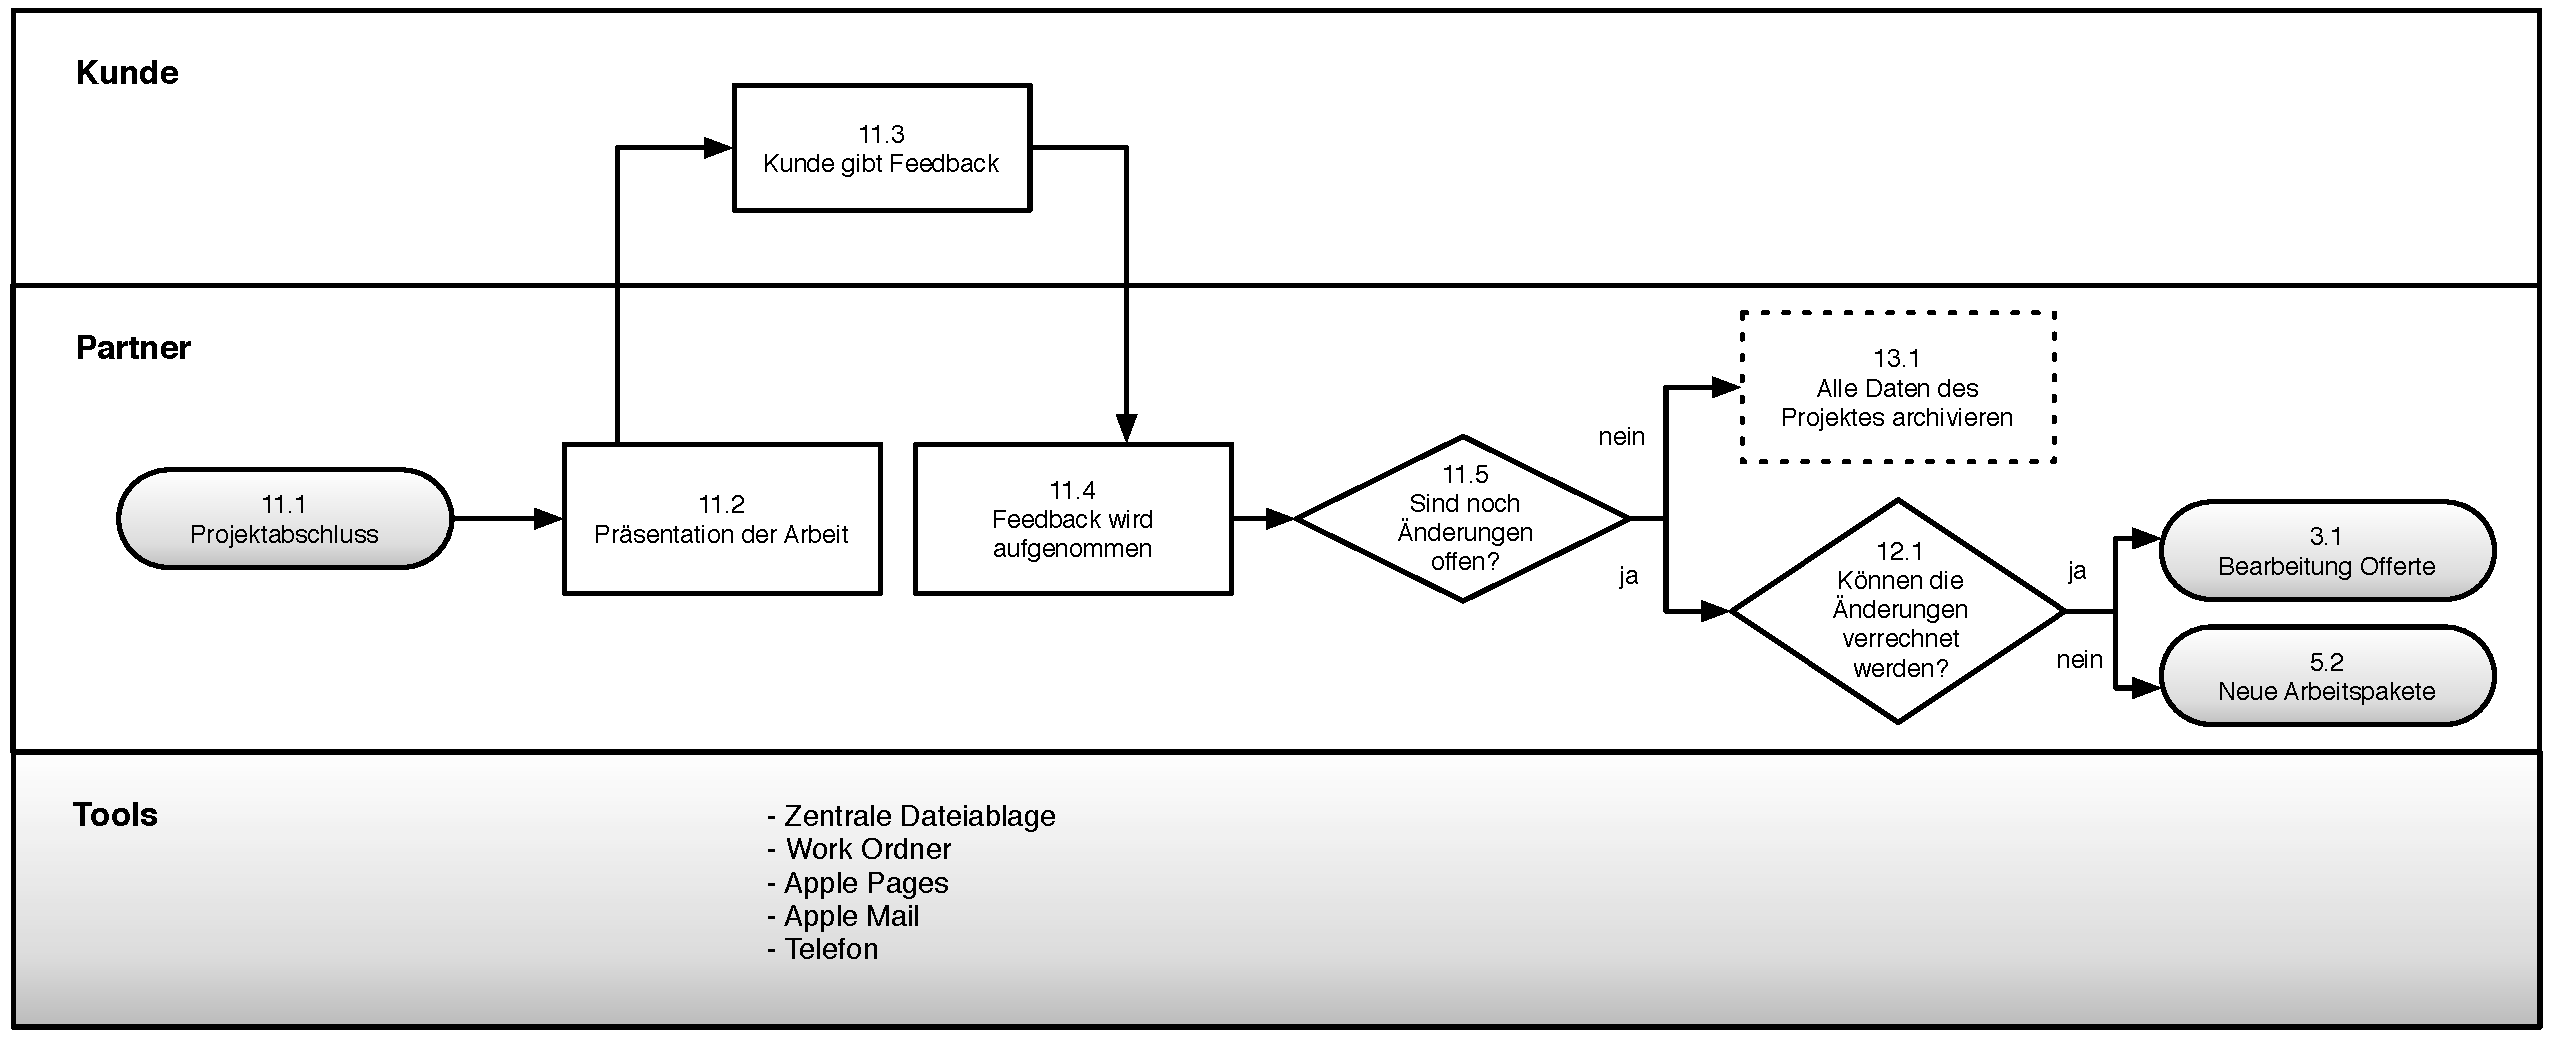
\includegraphics[width=0.99\textwidth,angle=0]{./bilder/analyse/03_ist_prozesse_abschluss_01.pdf}
\caption[Projektabschluss Prozess von allink 1/2]{Projektabschluss 
    Prozess von allink 1/2\footnotemark}
\label{pic:03_ist_prozesse_abschluss_01}
\end{center}
\end{figure}
\footnotetext{Eigene Darstellung}

\begin{figure}[p]
\begin{center}
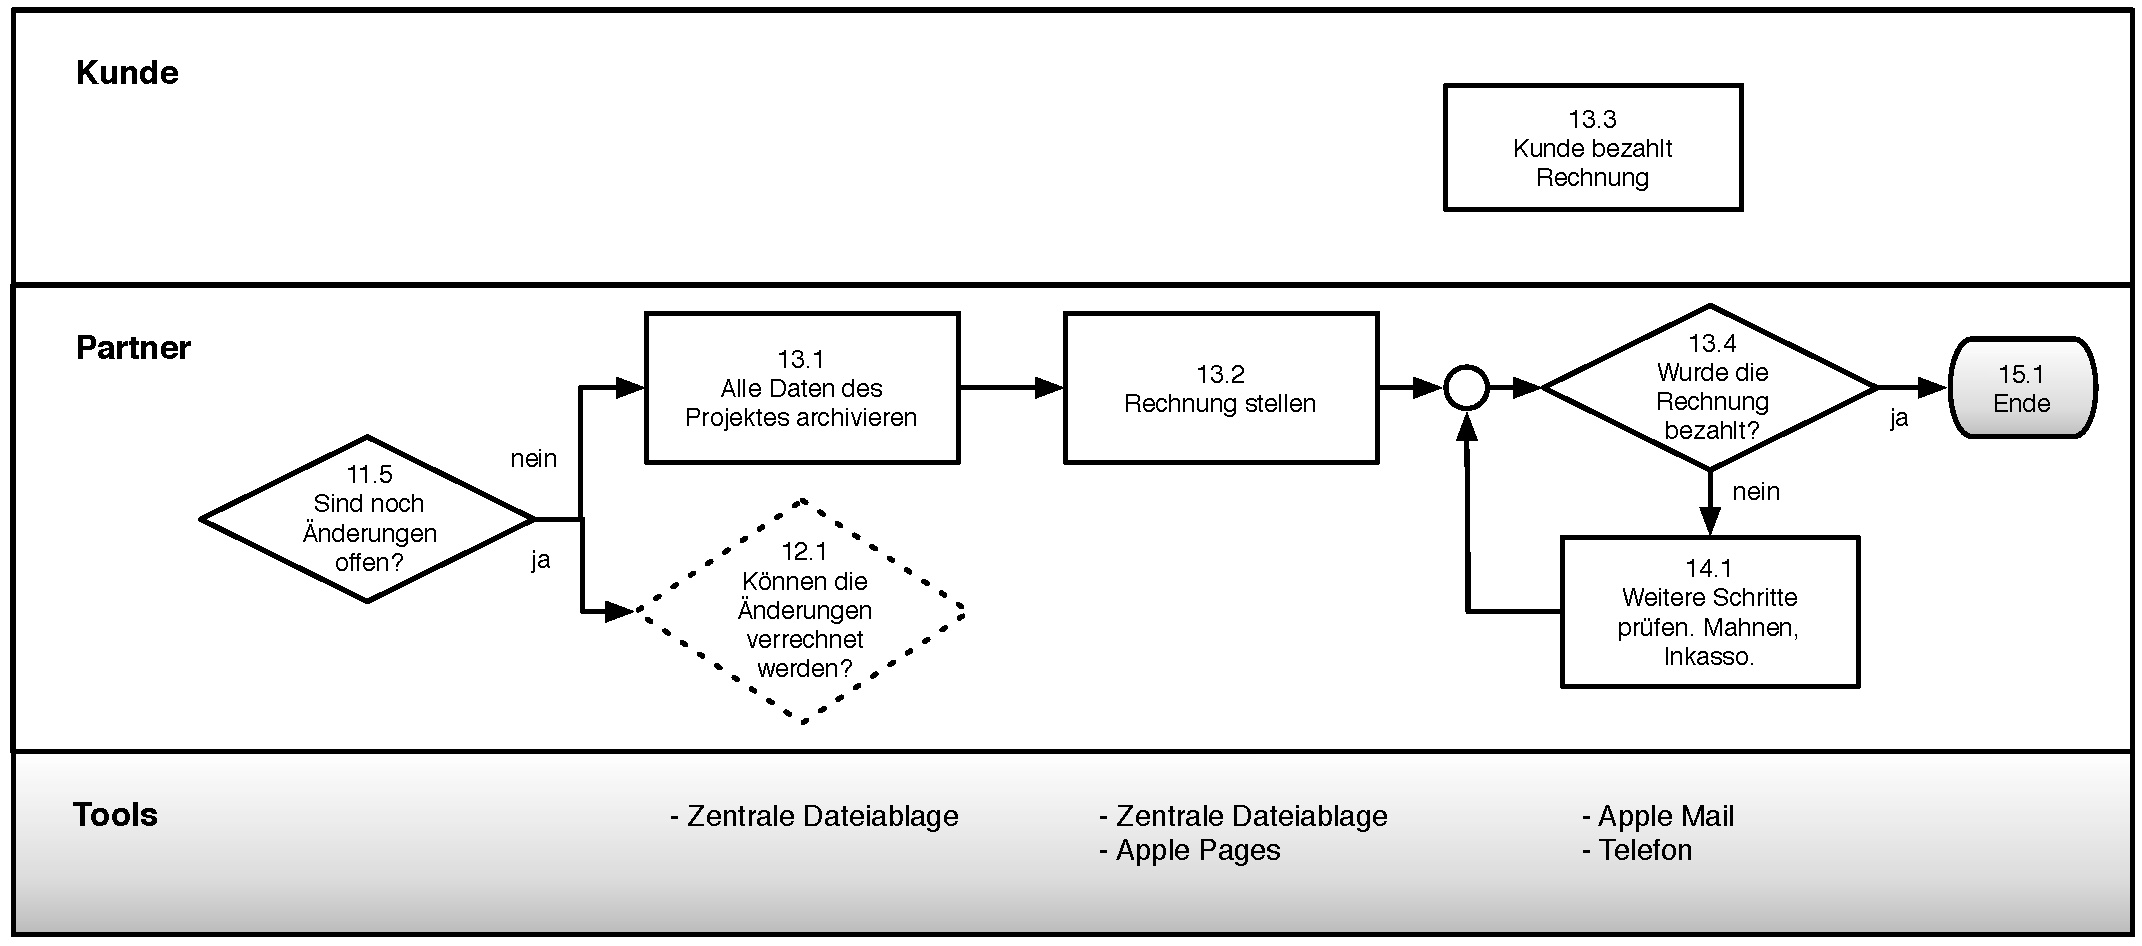
\includegraphics[width=0.99\textwidth,angle=0]{./bilder/analyse/03_ist_prozesse_abschluss_02.pdf}
\caption[Projektabschluss Prozess von allink 2/2]{Projektabschluss 
    Prozess von allink 2/2\footnotemark}
\label{pic:03_ist_prozesse_abschluss_02}
\end{center}
\end{figure}
\footnotetext{Eigene Darstellung}

In den Darstellungen \ref{pic:03_ist_prozesse_abschluss_01} und
\ref{pic:03_ist_prozesse_abschluss_02} ist der aktuelle Prozess des Projektabschlusses 
ersichtlich. Als erstes folgt nun die Präsentation der Arbeit beim Auftraggeber 
bzw. Kunden (\textbf{11.2}). Der Kunde gibt daraufhin Feedback (\textbf{11.3}), 
welches vom Projektleiter entgegengenommen und mit dem Kunden diskutiert wird (\textbf{11.4}).
Die in der Theorie empfohlenen Dokumente wie das Übergabe- und Übernahmeprotokoll
der Produktabnahme kommen zur Zeit gar nicht zur Anwendung.

Sofern dann noch Änderungen und Anpassungen nötig sind (\textbf{11.5}), stellt
der Projektleiter bzw. Partner wieder neuen Arbeitspakete zusammen und der
Bearbeitungsprozess beginnt von neuem (\textbf{5.2}). Wenn es sich bei den Wünschen
des Auftraggebers um neue, noch nicht bekannte, Anforderungen handelt, überprüft
der Partner ob eine Anpassung der Offerte notig ist (\textbf{12.1}).

Hier liegt es im Ermessen des Partners, ob es sinnvoll ist die zusätzlichen Kosten 
selbst zu tragen oder in Rechnung zu stellen. Je nach Projektverlauf, auf Grund von
Verzögerungen oder sonstigen Unannehmlichkeiten für den Auftraggeber, kann es
von Nutzen sein dem Kunden zu diesem Zeitpunkt entgegen zu kommen.

Wenn der Auftraggeber zufrieden ist und keine weiteren Anpassungen nötig sind, 
werden alle Daten des Projektes archiviert (\textbf{13.1}). Danach wird die
Endabrechnung durchgeführt und die Abschlussrechnung in Rechnung gestellt (\textbf{13.2}).
Im Verlauf der Zahlungsfrist bezahlt der Kunde die Rechnung (\textbf{13.3}).
Dies wird so lange überwacht (\textbf{13.4}) bis alle offenen Rechnungen beglichen
sind. Wenn eine Rechnung nach der Zahlungsfrist nicht bezahlt wurde, wird
geprüft ob weitere Schritte nötig sind (\textbf{14.1}).

In den meisten Fällen reichen ein paar zusätzliche Tage oder das Nachfragen beim 
Kunden. In den wenigsten Fällen muss gemahnt werden und das Einschalten eines 
Inkassounternehmens war in der Geschichte von allink zum Glück erst ein einziges 
mal notwendig. Sobald alle Rechnungen beglichen sind, gilt das Projekt definitiv 
abgeschlossen (\textbf{15.1}).

Zu diesem Zeitpunkt geschieht das Sammeln der Erfahrungsdaten aus dem Projekt,
wie in der Theorie beschrieben, nur implizit. Die Daten werden also nicht in 
einer Erfahrungsdatenbank gespeichert sondern existieren nur in den Köpfen
der Projektmitarbeiter.

\clearpage


\section{Verwendete Software}
Die Untersuchung der zur Zeit eingesetzten Sofware beschränkt sich auf jene,
die einen direkten Einfluss auf den aktuellen Projektablauf bei allink haben.
Es wird keine Software aufgelistet, die zur Erbringung der eigentlichen 
Dienstleistungen im Unternehmen eingesetzt wird.

In der Tabelle \ref{tab:verwendete_software} sind die verwendeten Tools
aufgelistet. Zu jeder Software wird der Hersteller, die Kategorisierung und der 
Verwendungszweck innerhalb von allink und dem Projektablauf angegeben. Danach
wird der Verwendungszweck für jede Software noch genauer umschrieben und wo
möglich mit einem Beispiel untermalt.

\begin{longtable}{lllp{6cm}}
    \toprule \textbf{Bezeichnung} & \textbf{Hersteller} & \textbf{Kategorie} & \textbf{Verwendungszweck} \\
    \midrule MacOS X & Apple & Betriebssystem & 
        \begin{minipage}[t]{6cm}
            \begin{compactitem}
                \item Über den ganzen Projektablauf
            \end{compactitem}
        \end{minipage}
        \\\\
    \midrule Microsoft Windows & Microsof & Betriebssystem & 
        \begin{minipage}[t]{6cm}
            \begin{compactitem}
                \item Tests während der Entwicklung
                \item Präsentation in der Abnahme
            \end{compactitem}
        \end{minipage}
        \\\\
    \midrule MacOS X Server & Apple & Betriebssystem &
        \begin{minipage}[t]{6cm}
            \begin{compactitem}
                \item Zentrale Dateiablage
                \item Server des Stundenwidgets
                \item Internes Wiki der Informatik
            \end{compactitem}
        \end{minipage}
        \\\\
    \midrule Apple iWork & Apple & Office Suite &
        \begin{minipage}[t]{6cm}
            \begin{compactitem}
                \item Kalkulation von Offerten
                \item Erstellung von Offerten
                \item Erstellung von Rechnungen und Briefschaften
            \end{compactitem}
        \end{minipage}
        \\\\
    \midrule Microsoft Office & Microsoft & Office Suite &
        \begin{minipage}[t]{6cm}
            \begin{compactitem}
                \item Informationsaustausch mit Kunden
            \end{compactitem}
        \end{minipage}
        \\\\
    \midrule Apple Mail & Apple & E-Mail Software &
        \begin{minipage}[t]{6cm}
            \begin{compactitem}
                \item Korrespondenz mit Kunden
                \item Interne Kommunikation
            \end{compactitem}
        \end{minipage}
        \\\\
    \midrule Stundenwidget & allink & Dashboardwidget &
        \begin{minipage}[t]{6cm}
            \begin{compactitem}
                \item Stundenrapportierung
            \end{compactitem}
        \end{minipage}
        \\\\
    \bottomrule
    \caption[Verwendete Software bei allink]{Verwendete Software bei allink\footnotemark}
    \label{tab:verwendete_software}
\end{longtable}
\footnotetext{Eigene Darstellung}

\subsubsection{MacOS X}
Als Hauptbetriebssystem verwendet allink MacOS X\footnote{Betriebssystem von Apple, \url{http://www.apple.com/macosx/}}.
Es läuft auf allen Arbeitsstationen der Mitarbeiter und Partner. Dies beruht
auf diversen Gründen. Grafiker arbeiten überwiegend mit MacOS X, da sich Apple
früh mit Adobe zusammenschloss um Werkzeuge für Grafiker zur Verfügung zu stellen.
Seit mehreren Jahren ist MacOS X auch für Entwickler wieder interessant. Die 
Mitarbeiter sind gemäss dem Auftraggeber sehr zufrieden damit und die Geschäftsleitung 
möchte dies zu diesem Zeitpunkt nicht in Frage stellen.

\subsubsection{Microsoft Windows}
Zusätzlich haben einige der Entwickler noch Microsoft Windows\footnote{Betriebssystem von Microsoft, \url{http://www.microsoft.com/windows/}}
über eine Virtualisierungslösung installiert. Dies wird zu überwiegend Testzwecken 
benötigt. Es existiert zu diesem Zeitpunkt aber kein Rechner, der ausschliesslich
mit Microsoft Windows arbeitet.

\subsubsection{MacOS X Server}
Auf dem Server der allink liegt das zentrale Dateiablagesystem. Die Zugriffsrechte können
auf dem Server für jede Freigabe definiert werden. So haben zum Beispiel
die Mitarbeiter keinen Zugriff auf den Administrationsordner der Geschäftsleitung.
Über diesen Server laufen auch die einzelnen Firmenkalender der Partner. Sie
können so gemeinsam Termine buchen und haben stets Einblick in die anderen
Kalender. Auch hier ist sich die Geschäftsleitung einig, zur Zeit keine 
Veränderung vorzunehmen.

\subsubsection{Apple iWork}
Für interne Zwecke setzt allink zur Zeit auf die Apple eigene Office Suite iWork\footnote{Office Suite von Apple, \url{http://www.apple.com/de/iwork/}}.
Pages wird überwiegend zur Erstellung von Offerten und Rechnungen verwendet. Mit Numbers
werden Tabellenkalkulationen wie die Liquiditätsplanung oder Lohnblätter erstellt.
Da dies aber von der Geschäftsleitung nie klar kommuniziert wurde, existieren
auch einige Excel Files, das Pendant der Microsoft Office Suite.

\subsubsection{Microsoft Office}
Da viele Kunden mit Microsoft Produkten arbeiten benötigt auch allink die
Office Suite\footnote{Microsoft Office für Mac, \url{http://www.microsoft.com/germany/mac}}, 
um Dateien mit Kunden ohne Interoperabilitätsprobleme austauschen zu können. 
Nicht jede Arbeitsstation verfügt zur Zeit über eine Installation. Da diese
Suite aber im Vergleich mit Apples iWork einiges teurer in den Anschaffung ist,
möchte die Geschäftsleitung diese über kurz oder lang nur noch auf einzelnen
Arbeitsstationen installieren.

\subsubsection{Apple Mail}
Apple Mail ist in das Betriebssytem von MacOS X integriert und wird gratis
mitgeliefert. Es verfügt über alle nötigen Funktionen, die eine E-Mail-Client-Software
heutzutage erfüllen muss. Auch diese möchte die Geschäftsleitung zur Zeit nicht
in Frage stellen.

\subsubsection{Stundenwidget}
Das Stundenwidget ist eine Eigenentwicklung von allink und läuft
im Dashboard\footnote{Widget Lösung von Apple, \url{http://www.apple.com/downloads/dashboard/}}
des Betriebssystems. Es ermöglicht Stunden auf ein Projekt zu buchen.
Die Daten werden auf dem eigenen Server gespeichert und pro Projekt abgelegt. Dieses Widget ist auf allen
Arbeitsstationen installiert und wird von den Mitarbeitern gelegentlich verwendet
um ihre Stunden auf ein Projekt zu rapportieren.


\section{Stärken und Schwächen}
In diesem Kapitel werden die Stärken und Schwächen des Unternehmens mit Fokus
auf den aktuellen Projektablauf genauer untersucht. Als Methode
wird die SWOT-Analyse\footnote{Die SWOT-Analyse ist ein Instrument um
Stärken, Schwächen, Chancen und Risiken darzustellen. Es eignet sich sowohl zur Situationsanalyse
wie auch als Instrument der Strategieformulierung. \citealp*[Vgl.][S. 134]{homburg2000quantitative}} 
verwendet und ist in der nachstehenden Grafik \ref{pic:swot_analyse} abgebildet.
Die einzelnen Punkte sind in Zusammenarbeit mit der Geschäftsleitung in einem Workshop
erarbeitet worden.

% Der Studierende ist sich bewusst, dass sich die Chancen und Risiken 
% nicht nur auf den Projektablauf sondern auf das ganze Unternehmen beziehen. 
% Da der Projektablauf jedoch ein Kernelement des Unternehmens ist, können sie 
% auch bei dieser Betrachtung verwendet werden.

\begin{figure}[htbp]
\begin{center}
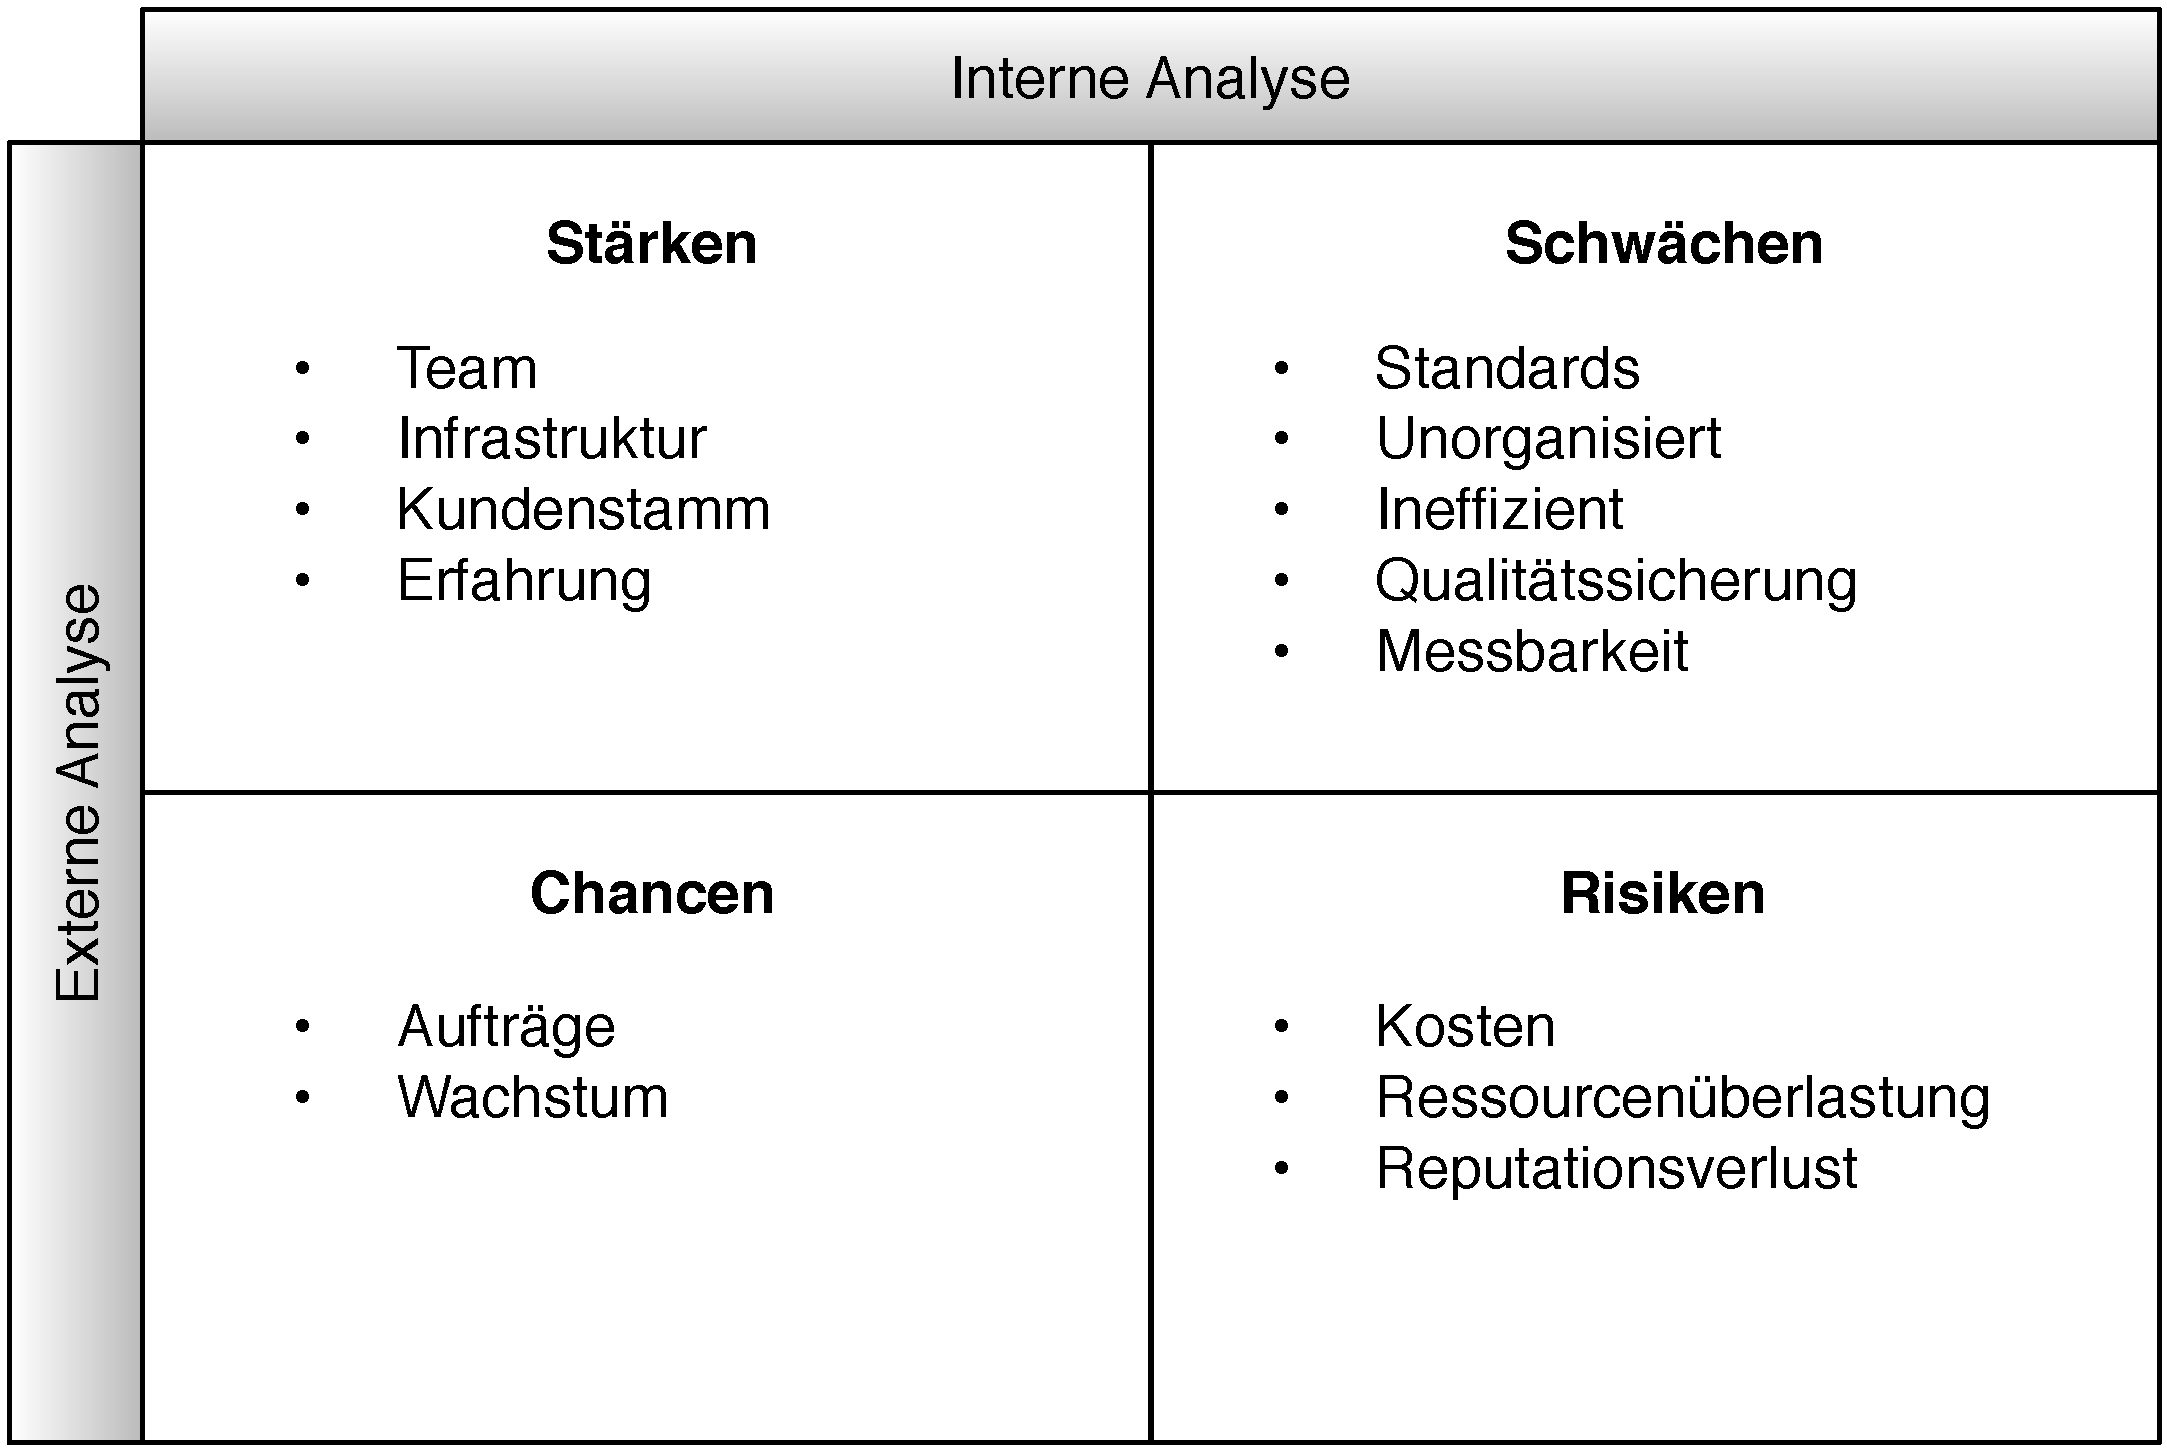
\includegraphics[width=0.8\textwidth,angle=0]{./bilder/analyse/swot_analyse.pdf}
\caption[SWOT-Analyse von allink]{SWOT-Analyse von allink\footnotemark}
\label{pic:swot_analyse}
\end{center}
\end{figure}
\footnotetext{Eigene Darstellung}

Es wird nun im Detail auf die einzelnen Punkte aus der SWOT-Analyse eingegangen
und wo möglich mit einem Beispiel aus der Praxis untermalt.

\subsection{Stärken}
Bei den Stärken handelt es sich um Eigenschaften des Unternehmens,
die es zu diesem Zeitpunkt mitbringt und teilweise noch nicht vollständig
ausnutzt. 

\subsubsection{Stabiles Team}
Das Unternehmen verfügt über ein starkes, ausgewogenes und interdisziplinäres Team. 
Sowohl im Bereich der Grafik wie auch der Informatik sind überaus fähige Mitarbeiter 
angestellt, deren Potenzial noch nicht vollständig ausgeschöpft wird. Die Beratung
befindet sich erst im Aufbau und das Unternehmen hat somit noch nicht ausreichend
Erfahrungen sammeln können. Die Mitarbeiter der Beratung sind jedoch ebenfalls
top motiviert, es ist jedoch noch zu früh um über die Fähigkeiten treffende
Aussagen machen zu können. Allgemein kann man das Team als extrem leistungswillig
bezeichnen, da sich alle zusammen mit der Agentur entwickeln möchten.

\subsubsection{Gute Infrastruktur}
Das Unternehmen verfügt über eine gute und moderne Infrastruktur. Kein Arbeitsgerät
ist älter als eineinhalb Jahre und überall sind die neusten Softwarepakete installiert.
Die allink legt grossen Wert auf gute Werkzeuge, da so die neusten Technologien
angewendet werden können und es daran nicht scheitern soll.

\subsubsection{Fundierte Erfahrung}
Durch die in den letzten fünf Jahren umgesetzten Projekte verfügt das Unternehmen
über einen grossen Erfahrungsschatz auf den es zurückgreifen kann. Das Hilft
überwiegend bei der Beratung von Kunden.
Auch verfügt das Unternehmen, wie man der Analyse der Kunden schon entnehmen
konnte, über einen relativ grossen Kundenstamm. Dies ist vor allem bei der
Akquisition sehr hilfreich, da man auf eine grosse Anzahl Referenzprojekte 
verweisen kann.

\subsection{Chancen}
Bei den Chancen handelt es sich um positive Auswirkungen, die zu erwarten sind,
wenn das Unternehmen die Schwächen in den Griff kriegt.

\subsubsection{Mehr Aufträge}
Der grosse Kundenstamm und die zur Zeit hohe Reputation des Unternehmens
birgt ein grosses Potenzial an neuen Aufträgen. Dabei ist das Potenzial der
Akquisition erst gering ausgeschöpft. Nur ein kleiner Prozentsatz der durchgeführten
Projekte in den letzten 5 Jahren wurde akquiriert. In den meisten Fällen entstanden
die Projekte durch direkte Anfragen von Kunden oder Partneragenturen.

\subsubsection{Gesundes Wachstum}
Die allink kann zur Zeit nicht alle Projektanfragen annehmen, da sie über zu
wenig Mitarbeiter verfügt. Es könnten mehr Mitarbeiter angestellt werden, dies
wurde aber bis anhin, durch die Anzeichen der Risiken die man schon mit dem bisherigen
Wachstum bewältigen muss, von der Geschäftsleitung vermieden.

\subsection{Schwächen}
Bei den Schwächen handelt es sich um Dinge die zur Zeit im Unternehmen nicht
optimal gelöst sind. Wenn diese nicht frühzeitig erkannt werden und nichts
dagegen unternommen wird, kann das die Entwicklung der Chancen verhindern und
das Eintreten der Risiken fördern.

\subsubsection{Fehlende Qualitätssicherung}
Durch die Überbelastung der Mitarbeiter können mit der Zeit die versprochenen Timings
nicht mehr eingehalten werden. Da die Ablagestrukturen nicht einheitlich geregelt
sind, kann es vorkommen, dass ein Mitarbeiter einem Kunden ein veraltetes oder
noch nicht freigegebenes Dokument sendet. Dies zieht einen zusätzlichen 
Mehraufwand mit sich, da man sich beim Kunden entschuldigen und rechtfertigen
muss. Zusätzlich strapaziert es auch die Beziehung zum Kunden.
Oft bleibt gegen Ende eines Projektes auch zu wenig Zeit die nötige 
Qualitätskontrollen durchzuführen, da man sich möglichst schnell um ein anderes,
möglicherweise auch schon überfälliges, Projekt kümmern muss. Der Kunde entdeckt
dann offensichtliche Fehler selbst und zweifelt zwangsläufig an der ganzen Arbeit.

\subsubsection{Mangelnde Effizienz}
Einfache Abläufe werden unnötig verkompliziert und geraten ins Stocken. Die ganze
Struktur wird langsam und ineffizient. Was sich wiederum negativ auf die zur
Verfügung stehende Zeit auswirkt.
Man hält vor, während und nach einem Projekt nur an wenige Standards fest. 
Das ganze Vorgehen ist nicht einheitlich, da in jedem Projekt wieder von
neuem entschieden wird, wie man vorgehen will. Es werden nur wenige einheitliche
Dokumente verwendet, zum Beispiel für die Erstellung von Offerten und Rechnungen.
Aber auch da entstehen schnell Fehler, zum Beispiel während der Umstellungen des 
Mehrwert Steuersatzes von 7.6\% auf 8\%. Da kein einheitliches Basistemplate
existiert, muss bei jeder Rechnung noch einmal sichergestellten werden, dass
der korrekte Steuersatz hinterlegt ist.

\subsubsection{Kein Controlling}
Auch bietet die fehlende bzw. chaotische Struktur nur wenige Punkte um Kennzahlen
zu messen. Den Umsatz den man mit dem Projekt erzielt hat ist zwar bekannt,
jedoch kann nur aus dem Gefühl heraus erahnt werden, ob mit dem Projekt einen
Gewinn für die Firma erzielt werden konnte. Die Mitarbeiter sind zwar angehalten
ihre Stunden in ein gemeinsames Stundenwidget einzutragen, jedoch werden
die Informationen nicht ausgewertet und können nicht mehr einzelnen Mitarbeitern
zugeordnet werden.

\subsection{Risiken}
Bei den Risiken handelt es sich um negative Auswirkungen, die zu erwarten sind,
wenn das Unternehmen die Schwächen nicht in den Griff bekommt.

\subsubsection{Hohe Kosten}
Durch die fehlende Kontrolle während eines Projektes, verliert man die
Übersicht über die Aufwände und schlussendlich die Kosten. Dadurch entsteht
ein Kostenrisiko, welches Konsequenzen für die Liquidität von allink haben kann.

\subsubsection{Ressourcenüberlastung}
Die Belastung für den Mitarbeiter wie auch für die Partner ist so über
längere Zeit nicht tragbar. Durch eine Überarbeitung kann es zu Ausfällen kommen, die
die Situation zusätzlich verschlimmern könnten. Das ganze Endet in einer 
schlechten Firmenkultur und das Unternehmung beginnt von Innen zu zerfallen.

\subsubsection{Reputationsverlust}
Da man Timings nicht mehr einhalten kann und man sich gegenüber dem Kunden
oft rechtfertigen muss entsteht ein schlechtes Bild der Unternehmung und sie
verliert an Vertrauen. Da die Konkurrenz im Tätigkeitsfeld der allink relativ
gross ist, ist ein möglicher Absprung und Angenturwechsel seitens des Kunden nicht 
auszuschliessen.


\section{Branchenvergleich}
\subsection{Fragekatalog}
Der in der Tabelle \ref{tab:fragekatalog} dargestellte Fragekatalog wurde für 
das Interview mit einer anderen Unternehmung aufgebaut. Die einzelnen Themenblöcke 
und die Zusammenstellung der Fragen wurden gezielt auf die Struktur der bestehenden 
Analyse der allink zusammengestellt um einen möglichst guten Vergleich darstellen 
zu können.

Als Interviewpartner werden möglichst ähnliche Agenturen wie die allink gesucht.
Optimal sind Agenturen, die die Herausforderung des Wachstums schon meistern
konnten. Der Studierende fragt in Zürich ein paar vergleichbare Agenturen an.

\newcounter{qcounter}
\begin{center}
    \begin{longtable}{lp{14cm}}
        \toprule \textbf{Nr.} & \textbf{Frage} \\
        \midrule & \textbf{Allgemeine Fragen} \\
        \midrule \addtocounter{qcounter}{1}\arabic{qcounter} & Wer ist mein Interviewpartner? \\
        \midrule \addtocounter{qcounter}{1}\arabic{qcounter} & Was ist die Funktion meines Interviewpartners? \\
        \midrule \addtocounter{qcounter}{1}\arabic{qcounter} & Was sind die Aufgaben meines Interviewpartners? \\
        \midrule & \textbf{Unternehmen} \\
        \midrule \addtocounter{qcounter}{1}\arabic{qcounter} & Wann wurde das Unternehmen gegründet? \\
        \midrule \addtocounter{qcounter}{1}\arabic{qcounter} & Wie viele Partner mit Mitspracherecht existieren? \\
        \midrule \addtocounter{qcounter}{1}\arabic{qcounter} & Wie ist das Organigramm des Unternehmens aufgebaut? \\
        \midrule \addtocounter{qcounter}{1}\arabic{qcounter} & Wie viele Vollzeitangstellte werden beschäftigt? \\
        \midrule \addtocounter{qcounter}{1}\arabic{qcounter} & Sind Praktikanten angestellt? \\
        \midrule \addtocounter{qcounter}{1}\arabic{qcounter} & Bietet das Unternehmen Lehrstellen an? \\
        \midrule & \textbf{Kunden} \\
        \midrule \addtocounter{qcounter}{1}\arabic{qcounter} & Wie viele Kunden sind Kleinstunternehmen? \\
        \midrule \addtocounter{qcounter}{1}\arabic{qcounter} & Wie viele Kunden sind kleine Unternehmen? \\
        \midrule \addtocounter{qcounter}{1}\arabic{qcounter} & Wie viele Kunden sind mittlere Unternehmen? \\
        \midrule \addtocounter{qcounter}{1}\arabic{qcounter} & Wie viele Kunden sind grosse Unternehmen? \\
        \midrule & \textbf{Projektablauf} \\
        \midrule \addtocounter{qcounter}{1}\arabic{qcounter} & Wie viele Projekte werden akquiriert? \\
        \midrule \addtocounter{qcounter}{1}\arabic{qcounter} & Wie viele Projekte entstehen durch direkte Anfragen? \\
        \midrule \addtocounter{qcounter}{1}\arabic{qcounter} & Wie werden die Aufwände eines potenziellen Projektes geschätzt? \\
        \midrule \addtocounter{qcounter}{1}\arabic{qcounter} & Wie wird auf Änderungen während des Projektes reagiert? \\
        \midrule \addtocounter{qcounter}{1}\arabic{qcounter} & Kommt es vor, dass Projekte während der Durchführung abgebrochen werden? \\
        \midrule \addtocounter{qcounter}{1}\arabic{qcounter} & Von wem werden die Arbeitspakete zusammengestellt? \\
        \midrule \addtocounter{qcounter}{1}\arabic{qcounter} & Wie werden die Arbeitspakete verteilt? \\
        \midrule \addtocounter{qcounter}{1}\arabic{qcounter} & Wie werden die Aufwände rapportiert? \\
        \midrule \addtocounter{qcounter}{1}\arabic{qcounter} & Wer kommuniziert direkt mit einem Kunden? \\
        \midrule \addtocounter{qcounter}{1}\arabic{qcounter} & Wie wird das Feedback eines Kunden verarbeitet? \\
        \midrule \addtocounter{qcounter}{1}\arabic{qcounter} & Wie wird mit zusätzlich zu verrechneten Anforderungen verfahren? \\
        \midrule \addtocounter{qcounter}{1}\arabic{qcounter} & Wie werden die Projektdaten archiviert? \\
        \midrule & \textbf{Verwendete Software} \\
        \midrule \addtocounter{qcounter}{1}\arabic{qcounter} & Auf welches Betriebssystem setzt das Unternehmen? \\
        \midrule \addtocounter{qcounter}{1}\arabic{qcounter} & Welche Office Suite setzt das Unternehmen ein? \\
        \midrule \addtocounter{qcounter}{1}\arabic{qcounter} & Was für Projektmanagement-Software wird verwendet? \\
        \midrule & \textbf{Stärken und Schwächen} \\
        \midrule \addtocounter{qcounter}{1}\arabic{qcounter} & Wo liegen die Stärken des Unternehmens? \\
        \midrule \addtocounter{qcounter}{1}\arabic{qcounter} & Wo sieht das Unternehmen ihre Chancen? \\
        \midrule \addtocounter{qcounter}{1}\arabic{qcounter} & Wo liegen die Schwächen des Unternehmens? \\
        \midrule \addtocounter{qcounter}{1}\arabic{qcounter} & Mit was für Risiken sieht sich das Unternehmen konfrontiert? \\
        \bottomrule
        \caption[Fragekatalog zur Marktanalyse]{Fragekatalog zur Marktanalyse\footnotemark}
        \label{tab:fragekatalog}
    \end{longtable}
\end{center}
\footnotetext{Eigene Darstellung}

Der erstellte Fragenkatalog dient als Leitfaden im Interview. Die Antworten
werden entgegengenommen, diskutiert und anschliessend in beschreibender Form
dokumentiert. Die verweisenden Fragen werden in Klammern an der dazugehörigen
Textstelle angegeben. Falls gewissen Fragen nicht beantwortet wurden, wird dies 
erwähnt und begründet.

\subsection{Panter IIc}
Das Unternehmen Panter IIc mit Sitz in Zürich hat sich freundlicherweise dazu
bereiterklärt mit dem Studierenden ein Interview durchzuführen. Der Interview
Partner ist Syrus Mozafar. Er ist Teilhaber der Panter IIc und Mitglied der
Geschäftsleitung (\textbf{1}).

Er ist laut eigenen Angaben auch für das Projektmanagement zuständig (\textbf{2})
und oft selbst Projektleiter. Sein Aufgabenbereich liegt speziell in der 
Projektplanung, Konsolidierung der Ressourcenplanung und das Auszahlen von
Löhnen in der Buchhaltung (\textbf{3}).

\subsubsection{Unternehmen}
Das Unternehmen ist im Jahre 2005 als GmbH gegründet worden. Die Rechtsform
ist bis heute erhalten geblieben (\textbf{4}). Es existieren fünf Teilhaber,
jedoch kann in ihrer Firmenkultur jeder Mitarbeiter bei grösseren Entscheidungen
des Unternehmens mitentscheiden (\textbf{5}).

Es existiert zur Zeit kein richtiges Organigramm, die Struktur ist flach
und jeder Mitarbeiter hat gewisse Kompetenzen und Aufgaben (\textbf{6}). 
Insgesamt hat Panter zwölf Mitarbeiter und zusätzliche sechs Mitarbeiter im
Personalverleih. Die Anstellungspensum variiert zwischen 20\% bis 80\% (\textbf{7}).
Zur Zeit werden weder Praktikanten noch Lehrlinge beschäftigt und die Geschäftsleitung
wird dies zu diesem Zeitpunkt nicht ändern, da sie darin eher einen Mehraufwand
als Nutzen sehen (\textbf{8} und \textbf{9}).

\subsubsection{Kunden}
Panter verfügt über einen relativ grossen Kundenstamm. Die Verteilung
der Unternehmensgrössen der Kunden unterteilen sich in ca. 40\% Kleinstunternehmen,
20\% kleine Unternehmen, 10\% mittlere Unternehmen und 30\% grosse
Unternehmen (\textbf{10} bis \textbf{13}).

\subsubsection{Projektablauf}
Bei Panter werden ca. 20\% der Projekte selbst akquiriert (\textbf{14}) und ca.
80\% entstehen durch direkte Anfragen oder Folgeaufträge (\textbf{15}). Kleinere
Projekte mit einem Umsatzvolumen bis 20'000 CHF werden nur grob im Alleingang
des Projektleiters geschätzt. Bei grösseren Projekten werden auf Grund der
Technologiewahl Experten innerhalb von Panter oder ausserhalb herbeigezogen
um eine möglichst genaue Schätzung abgeben zu können (\textbf{16}). Sie verwenden
dazu keine speziellen Verfahrenstechniken und setzen überwiegend die Software
Microsoft Excel ein. Bei grösseren Änderungen während eines Projektes wird
erneut eine Schätzung vorgenommen und dem Kunden die zusätzlichen Aufwände
offeriert (\textbf{17}). Es wird von Fall zu Fall entschieden ob eine Änderung 
zusätzlich verrechnet oder dem Kunden ``geschenkt'' wird (\textbf{24}). Bis zu 
diesem Zeitpunkt kam es erst einmal zu einem vollständigen Abbruch eines Projektes 
während dessen Durchführung (\textbf{18}).

Die Arbeitspakete werden überwiegend während der Erstellung der Schätzung und 
der Offerte vom Projektleiter und den Experten zusammengestellt (\textbf{19}).
Dabei ist im Normalfall immer auch eine Person der Geschäftsleitung vertreten.
Die Arbeitspakete werden dann auch gleich von dieser Gruppe an die für das 
Projekt eingeplanten Ressourcen verteilt (\textbf{20}).

Die Aufwände werden von den Mitarbeitern sehr exakt rapportiert (\textbf{21}),
da die Lohnsummen der einzelnen Mitarbeiter von den Anzahl geleisteten Stunden
abhängt. Es existieren somit keine Fixlöhne bei Panter.

Die Kommunikation mit dem Kunden erfolgt im Normalfall über den Projektleiter.
Es kommt aber auch vor, dass ein Mitarbeiter direkt bei einem Kunden zusätzliche
Informationen einfordert (\textbf{22}). Es existieren keine fixen Regeln dazu.
Das Feedback des Kunden wird im Unternehmens Wiki eingetragen. Da die zerstreute
Verteilung der Projektdaten in der Vergangenheit schon öfters bemängelt wurde, 
baut Panter zu diesem Zeitpunkt eine Struktur für ein Projektarchiv auf. Sie
verwenden zudem ein allgemeines E-Mail Konto um projektspezifische E-Mails
zentral und für alle Mitarbeiter zugänglich abzulegen (\textbf{23} und \textbf{25}).

\subsubsection{Verwendete Software}
Das Unternehmen setzt auf kein spezifisches Betriebssystem. Jeder Mitarbeiter
hat sein eigenes Gerät mit seinem präferierten System installiert. Einzig für
die unternehmenseigenen Server wird das Betriebssystem Debian\footnote{Debian 
ist ein frei verfügbares Betriebssystem, \url{http://www.debian.org/}} 
vorausgesetzt (\textbf{26}).

Also Office Suite setzt Panter auf die Open-Source
Lösung OpenOffice\footnote{OpenOffice ist eine frei verfügbare Office Suite, 
\url{http://de.openoffice.org/}}. Zusätzlich, um Interoperabilitätsprobleme
mit Kunden zu vermeiden, hat Panter eine Arbeitsstation mit Microsoft Windows
und Microsoft Office ausgerüstet (\textbf{27}).

Panter setzt überwiegend auf die Projektmanagement Software RedMine\footnote{RedMine
ist eine Webapplikation für Projektmanagement, \url{http://www.redmine.org/}},
wobei sie nicht vollständig sondern nur Teile davon nutzen (\textbf{28}). 
Das unternehmenseigene Wiki und diverse Exceldokumente unterstützen die in RedMine
verwalteten Projekte. 

\subsubsection{Stärken und Schwächen}
Die Stärken sieht Panter zur Zeit überwiegend in ihrer Grösse und der flachen
Struktur. Mit dieser können ihre Projekte zur Zeit sehr erfolgreich durchgeführt 
werden. Auch sehen sie das Mitspracherecht aller Mitarbeiter als grossen Vorteil.
Zusätzlich sei auch die verwendete und moderne Technologie bis jetzt immer
ein grosser positiver Faktor gewesen (\textbf{29}).

Chancen sehen sie ebenfalls im Wachstum der Agentur und allgemein könnten
sie effizienter werden. Die Schätzverfahren können noch verbessert werden und
in Zukunft möchten sie mehr auf Leistung und nicht pauschal verrechnen können (\textbf{30}).

Die Schwächen liegen hingegen bei den nicht vollständig geregelten 
Verantwortungsbereichen und dass sie keine Cashcow\footnote{Als Cashcow bezeichnet
man in der Betriebswirtschaftslehre ein Produkt oder einen Kunden, mit dem man
laufend hohe Gewinne erwirtschaften kann.} besitzen (\textbf{31}).

Als Risiko sehen sie die schwankende Liquiditätsplanung, die nur auf zwei Monate 
hinaus garantiert werden kann. Zusätzlich fürchten sie eine negative Veränderung 
der Firmenkultur bei einem weiteren Wachstum (\textbf{32}).

\subsection{FEINHEIT GmbH}

\subsubsection{Unternehmen}

\subsubsection{Kunden}

\subsubsection{Projektablauf}

\subsubsection{Verwendete Software}

\subsubsection{Stärken und Schwächen}


\section{Zwischenfazit}
Panter: auch 5 Teilhaber, aber alle dürfen mitreden.
Panter: Keine Aufteilung in Bereiche, flache Struktur.
Panter: Weder Praktikanten noch Lehrlinge, da Mehraufwand befürchtet.
Panter: Prozentual mehr grosse Unternehmen, aber ähnlich.
Panter: noch kein Projektarchiv, work ordner System


% \subsection{Methode zur Analyse}
% \subsubsection{Vorgehensmodell nach Grochla}
% Zur Erstellung meiner Ist-Analyse verwende ich die ersten drei Phasen des 
Vorgehensmodell von Erwin Grochla\cite[S. 44-74]{grochla1982grundlagen}.
Die weiteren vier Phasen führen über eine Analyse hinaus und kommen
nicht zur Anwendung.

\subsubsection{Voruntersuchung}
In der Voruntersuchung, auch Pilotstudie genannt, stellt man sich Fragen wie
``Was soll geändert werden?'' und ``Welches sind die Ziele?''. Man verschafft
sich einen Grobüberblick über das eigentliche Problem und die Rahmenbedingungen
möglicher Lösungen. Auch entscheidet man in der Voruntersuchung, ob der Prozess
fortgesetzt oder abgebrochen werden soll. In der Voruntersuchung können die 
meisten Analyse- und Bewertungstechniken verwendet werden.

Nach Absprache mit dem Auftraggeber werde ich mir zur Voruntersuchung mit  
Hilfe von MindMaps einen besseren Überblick über die aktuellen Probleme bei
allink verschaffen. Auf die einzelnen Punkte soll genauer eingegangen
und wenn möglich Fallbeispiele aus der Praxis genannt werden.

Ich verwende die Technik der MindMaps schon seit einigen Jahren und verwende
sie sehr oft in Projekten um mir einen Überblick über Themen zu verschaffen.

\begin{quote}
Eine Mind-Map beschreibt eine besonders von Tony Buzan geprägte kognitive 
Technik, die z.B. zur Erschliessung und visuellen Darstellung eines Themengebietes, 
zur Planung oder für Mitschriften genutzt werden kann. Hierbei soll das Prinzip 
der Assoziation helfen, Gedanken frei zu entfalten und die Fähigkeiten des Gehirns 
zu nutzen. Die Mind-Map wird nach bestimmten Regeln erstellt und gelesen. Den 
Prozess bzw. das Themengebiet bzw. die Technik bezeichnet man als Mind-Mapping.
\cite{wikipedia_mindmap}
\end{quote}

\subsubsection{Ist-Aufnahme}
In der zweiten Phase erfasst man den aktuellen Zustand indem man das zu 
Untersuchende aus möglichst vielen Betrachtungswinkeln analysieren. Zu den
Techniken der Ist-Aufnahme zählen die Selbstaufschreibung, die Befragung und 
die Beobachtung.

Ich werde mit mir selbst eine Selbstaufschreibung durchführen, da ich in meinem 
Arbeitsalltag unseren Problemen genau so ausgesetzt bin. Aber da mir nur begrenzt
Zeit zur Verfügung steht und damit die Mitarbeiter möglichst ungestört arbeiten
können, begrenze ich Befragungen auf die Partner. Die Meinungen und Beobachtungen
aller Partner fliesst dann in die Ist-Aufnahme ein.

\subsubsection{Ist-Kritik}
In der dritten Phase widmet man sich den erhobenen Informationen aus der zweiten Phase. 
Die genauen Ursachen der Probleme sollen herausgeschält werden, damit nicht nur 
Symptome behandelt werden. 

Um die Probleme auf ihre tatsächlichen Ursachen zurückführen zu können,
werde ich eine Form der Prüfmatrix, eine Problem-Ursachen Matrix, erstellen.

\begin{quote}
    Die Prüfmatrix ist ein vereinfachtes Verfahren um Mängel und deren Ursachen 
    zu ermitteln. Mängel werden dabei möglichen Ursachenkategorien matrixförmig 
    gegenübergestellt. Im Schnittpunkt von Mangel und Ursachenkategorie werden 
    die tatsächlichen Ursachen gesucht.\cite{schmidt2000methode}
\end{quote}

  
  \chapter{Bedürfnisse und Anforderungen}\label{chap:anforderungen}
  Bei der Aufnahme der Anforderungen zusammen mit der Geschäftsleitung der allink
wird darauf geachtet, dass die Anforderungen so einfach und eindeutig wie möglich
formuliert werden. Zusätzlich wird jede Anforderung beschrieben, wo nötig begründet 
und soweit auf ihre Machbarkeit geprüft, wie es zu diesem Zeitpunkt möglich ist.
Die Anforderungen werden priorisiert, indem sie in Muss- und Kann-Anforderungen 
kategorisiert werden.\footnote{\citealp*[Vgl.][S. 32]{hobel2006gabler}} 

\newcounter{acounter}

\section{Stakeholder}

\subsection{Kunde}
Die in der Tabelle \ref{tab:anforderungen_stakeholder_kunde} aufgelisteten 
Anforderungen sind von der Geschäftsleitung der allink formuliert, jedoch
aus der Sicht des Kunden gesehen.

\begin{table}[htbp]
\begin{center}
    \begin{tabular}{llp{8cm}l}
        \toprule \textbf{Nr.} & \textbf{Anforderung} & \textbf{Beschreibung} & \textbf{Priorisierung} \\
        \midrule \addtocounter{acounter}{1}\arabic{acounter} & ... & ... & Muss \\
        \midrule \addtocounter{acounter}{1}\arabic{acounter} & ... & ... & Muss \\
        \bottomrule
    \end{tabular}
    \caption{Anforderungen an das neue Projektmanagement seitens des Kunden}
    \label{tab:anforderungen_stakeholder_kunde}
\end{center}
\end{table}

\subsection{Geschäftsleitung}

\begin{table}[htbp]
\begin{center}
    \begin{tabular}{llp{8cm}l}
        \toprule \textbf{Nr.} & \textbf{Anforderung} & \textbf{Beschreibung} & \textbf{Priorisierung} \\
        \midrule \addtocounter{acounter}{1}\arabic{acounter} & ... & ... & Muss \\
        \midrule \addtocounter{acounter}{1}\arabic{acounter} & ... & ... & Muss \\
        \bottomrule
    \end{tabular}
    \caption{Anforderungen an das neue Projektmanagement seitens der Geschäftsleitung}
    \label{tab:anforderungen_stakeholder_partner}
\end{center}
\end{table}

\subsection{Mitarbeiter}

\begin{table}[htbp]
\begin{center}
    \begin{tabular}{llp{8cm}l}
        \toprule \textbf{Nr.} & \textbf{Anforderung} & \textbf{Beschreibung} & \textbf{Priorisierung} \\
        \midrule \addtocounter{acounter}{1}\arabic{acounter} & ... & ... & Muss \\
        \midrule \addtocounter{acounter}{1}\arabic{acounter} & ... & ... & Muss \\
        \bottomrule
    \end{tabular}
    \caption{Anforderungen an das neue Projektmanagement seitens der Mitarbeiter}
    \label{tab:anforderungen_stakeholder_mitarbeiter}
\end{center}
\end{table}

\subsection{Drittanbieter}

\begin{table}[htbp]
\begin{center}
    \begin{tabular}{llp{8cm}l}
        \toprule \textbf{Nr.} & \textbf{Anforderung} & \textbf{Beschreibung} & \textbf{Priorisierung} \\
        \midrule \addtocounter{acounter}{1}\arabic{acounter} & ... & ... & Muss \\
        \midrule \addtocounter{acounter}{1}\arabic{acounter} & ... & ... & Muss \\
        \bottomrule
    \end{tabular}
    \caption{Anforderungen an das neue Projektmanagement seitens der Drittanbieter}
    \label{tab:anforderungen_stakeholder_drittanbieter}
\end{center}
\end{table}

% \section{Nicht funktionale Anforderungen}
% \section{Funktionale Anforderungen}
\section{Kennzahlen}

\begin{table}[htbp]
\begin{center}
    \begin{tabular}{llp{8cm}l}
        \toprule \textbf{Nr.} & \textbf{Anforderung} & \textbf{Beschreibung} & \textbf{Priorisierung} \\
        \midrule \addtocounter{acounter}{1}\arabic{acounter} & ... & ... & Muss \\
        \midrule \addtocounter{acounter}{1}\arabic{acounter} & ... & ... & Muss \\
        \bottomrule
    \end{tabular}
    \caption{Kennzahlen-Anforderungen an das neue Projektmanagement}
    \label{tab:anforderungen_stakeholder_kennzahlen}
\end{center}
\end{table}
  
  \chapter{Konzept}\label{chap:konzept}
  \section{Varianten}
  \subsubsection{Variante 1}
  \subsubsection{Variante 2}
  \subsubsection{Variante 3}
  \section{Nutzwertanalyse}
  
  \chapter{Proof of Concept}\label{chap:proof_of_concept}
  
  \chapter{Reflektion}\label{chap:reflektion}
  \section{Fazit}
  \section{Ausblick}
  \section{Danksagung}
  
  \appendix
  
  \chapter{Rahmenbedingungen}
  Für das Informatik Diplomstudium an der Fachhochschule Zürich für Technik
HSZ-T wird von den Studenten verlangt eine Diplomarbeit eigenständig zu
verfassen.

\section{Sprache}
Die Semesterarbeit wurde in deutscher Sprache verfasst. Englische Ausdrücke 
wurden immer dort verwendet, wo diese im Sprachgebrauch in den verwendeten 
Programmen genau so gebraucht werden.

Aus Gründen der besseren Lesbarkeit der Diplomarbeit wurde teilweise auf 
die Nennung beider Geschlechter verzichtet. In diesen Fällen ist die 
weibliche Form ausdrücklich inbegriffen.
  
\section{Richtlinien}
Folgende Dokumente mit Richtlinien der Hochschule für Technik Zürich 
wurden für die Diplomarbeit berücksichtigt:

\begin{itemize}
    \item Reglement\footnote{\citealp*[Vgl.][ganzes Dokument]{hsz_reglement}}
    \item Ablauf\footnote{\citealp*[Vgl.][ganzes Dokument]{hsz_ablauf}}
    \item Bewertungskriterien\footnote{\citealp*[Vgl.][ganzes Dokument]{hsz_bewertungskriterien}}
\end{itemize}

  
  \chapter{Aufgabenstellung}\label{chap:aufgabenstellung}
  \section{Ausgangslage}
Die Agentur allink.creative ist im letzten Jahr stark gewachsen. Von zehn
Mitarbeitern im Februar 2010 auf siebzehn Mitarbeiter im Februar 2011. Dies hat 
zur Auswirkung, dass gewisse Funktionen und Prozesse neu definiert und bestehende
überarbeitet werden müssen, um weiterhin effizient, oder wenn möglich noch 
effizienter, arbeiten zu können. Die Agentur arbeitet überwiegend mit Apple
Computern und setzt gewisse Software ein, die die Geschäftsleitung beibehalten 
möchte. Die konkreten Vorstellungen und Vorgaben müssen von dem Studierenden
in der Arbeit erfasst werden.

\section{Ziel der Arbeit}
Bereiche wie die Stundenrapportierung, die Projektplanung und das Projektcontrolling 
können mit Hilfe von IT-Lösungen massgebend optimiert und vereinfacht werden. 
In dieser Arbeit sollen die Herausforderungen, die der Auftraggeber in der 
Planung und im Controlling eines Projektes zu bewältigen hat, erfasst und 
Lösungsvorschläge evaluiert werden. Der Fokus liegt dabei auf der besseren 
Messbarkeit des finanziellen Erfolges eines Projektes und des gesamten 
Unternehmens.

Die Arbeit grenzt sich ganz klar von der Finanzbuchhaltung ab, da
diese keinen direkten Einfluss auf die Projekte hat und bei allink.creative 
bei einen Treuhänder ausgelagert wurde.

\section{Aufgabenstellung}
Folgende Aufgaben soll der Studierende während dieser Arbeit bewältigen:

\begin{itemize}
    \item Ist-Situation im Bereich Projektablauf der allink.creative erfassen
    \item Anforderungen an den neuen Prozess festlegen. Unteranderem Kennzahlen 
        definieren, die in Zukunft auf Projektebene gemessen werden sollen
    \item Eine Recherche der Prozesse in ähnlich funktionierenden KMUs durchführen
    \item Neue Prozesse definieren und bestehende überdenken
    \item Evaluation von IT-Lösungen, die diese Prozesse möglichst passend 
        für den Auftraggeber abbilden und die definierten Kennzahlen generieren können
\end{itemize}

\section{Erwartete Resultate}
Der Studierende soll dem Auftraggeber ein Dokument erstellen, das folgende 
Punkte beinhaltet: 

\begin{itemize}
    \item Beschreibung der Ist-Situation im Bereich Projektablauf
    \item Übersicht der bestehenden Software beim Auftraggeber
    \item Anforderungen an den neuen Prozess inkl. Kennzahlen, die auf 
        Projektebene gemessen werden sollen
    \item Konzept des neuen und überarbeiteten Prozesses
    \item Übersicht der bestehenden Software in der neuen Prozesslandschaft
    \item Softwareempfehlungen für die komplette Prozessabbildung
    \item ``Make or Buy''-Entscheid mit dem Auftraggeber
\end{itemize}

Sobald der neue Prozess und die Tools definiert sind und der Auftraggeber 
einen Entscheid gefällt hat, soll anhand
eines realen Projektes ein ``Proof of Concept'' erstellt werden.

\section{Abgrenzung}
Folgende Punkte werden abgegrenzt, da sie den Rahmen der Arbeit Überschreiten 
würden:

\begin{itemize}
    \item Die Analysen beschränken sich auf Recherchen im Internet und Büchern
    \item Umfragen, Erhebungen sowie Feldstudien werden nicht durchgeführt
\end{itemize}


  
  \chapter{Detailanalyse der Aufgabenstellung}
In der Detailanalyse der Aufgabenstellungen werden die zu bewältigenden
Aufgaben und deren erwartete Resultate ausformuliert.

\section{Aufgaben und Resultate}
\subsubsection{Ist-Situation im Bereich Projektablauf der allink.creative erfassen}
Es soll eine Beschreibung des aktuellen Projektablaufes der allink erarbeitet
und möglichst vollständig alle heutigen Prozessschritte dargestellt und die Vor- 
und Nachteile des Projektablaufes aufgezeigt werden. Hinzu kommt die darin verwendete Software und
deren Einsatzzweck.
\\\\
\underline{Erwartete Resultate}

\begin{description}
    \item[R1] Beschreibung der Ist-Situation im Bereich Projektablauf
    \item[R2] Übersicht der bestehenden Software beim Auftraggeber
\end{description}

\subsubsection{Kennzahlen definieren, die in Zukunft auf Projektebene gemessen werden sollen}
Zusammen mit dem Auftraggeber sollen Voraussetzungen, unteranderem Kennzahlen,
definiert werden, die bei der Erarbeitung des neuen Projektablaufes berücksichtig
werden müssen. 
\\\\
\underline{Erwartete Resultate}

\begin{description}
    \item[R3] Anforderungen an den neuen Prozess inkl. Kennzahlen, die auf 
        Projektebene gemessen werden sollen
\end{description}
  
\subsubsection{Eine Recherche der Prozesse in ähnlich funktionierenden KMUs durchführen}
Der Studierende soll in Gesprächen mit anderen KMUs recherchieren, was Agenturen
mit ähnlichen Voraussetzungen und Herausforderungen wie allink für Projektabläufe
und Hilfsmittel verwenden.
\\\\
\underline{Erwartete Resultate}

Die Informationen aus den Recherchen sollen in den Lösungsvorschlag eingearbeitet
und berücksichtigt werden.

\subsubsection{Neue Prozesse definieren und bestehende, sofern sinnvoll, überarbeiten}
Anhand den bis dahin gewonnen Erkenntnissen soll der bestehende Projektablauf
überarbeitet und neu definiert werden. Dazu arbeitet der Studierende eng mit
dem Auftraggeber zusammen, damit sichergestellt ist, dass eine in der Realität
umsetzbare Lösung definiert wird.
\\\\
\underline{Erwartete Resultate}

\begin{description}
    \item[R4] Konzept des neuen und überarbeiteten Prozesses
    \item[R5] Übersicht der bestehenden Software in der neuen Prozesslandschaft
    \item[R6] Softwareempfehlungen für die komplette Prozessabbildung
\end{description}

\subsubsection{Evaluation von IT-Lösungen, die diese Prozesse möglichst passend 
    für den Auftraggeber abbilden und die definierten Kennzahlen generieren können}
Sofern die bestehende Software des Auftraggebers nicht ausreicht um den neuen
Projektablauf im Unternehmen umzusetzen, soll der Studierende alternative 
Lösungen evaluieren. Darin können auch selbst umzusetzende Tools empfohlen 
werden, sofern der Aufwand für dessen Entwicklung gerechtfertigt ist.
\\\\
\underline{Erwartete Resultate}

\begin{description}
    \item[R7] ``Make or Buy''-Entscheid mit dem Auftraggeber
\end{description}

\section{Aufwandschätzung}
Aufgrund den Anforderungen an die Diplomarbeit und aus der Aufgabenstellung
ergeben sich Arbeitspakete, die in eine Planungs- und Umsetzungsphase
der Diplomarbeit unterteilt werden. Auch versuche ich den Aufwand der einzelnen
Arbeitspaketen in Stunden zu schätzen und diese dann in eine realistische 
Projektplanung einfliessen zu lassen.

\subsection{Planungsphase}
Die Arbeitspakete, die vor der Freigabe der Diplomarbeit erbracht werden müssen,
sind in Stunden geschätzt und in der Tabellen \ref{tab:auwand_planungsphase} 
aufgelistet.

\begin{table}[htbp]
\begin{center}
    \begin{tabular}{llc}
        \toprule & \textbf{Arbeitspaket} & \textbf{Aufwand in Stunden} \\
        \midrule \textbf{P1} & Thema evaluieren & 16 \\
        \midrule \textbf{P2} & Aufgabenstellung ausarbeiten & 8 \\
        \midrule \textbf{P3} & Betreuer finden & 8 \\
        \midrule \textbf{P4} & Kick-Off vorbereiten & 12 \\
        \bottomrule & \textbf{Total Stunden} & \textbf{44} \\
        \bottomrule
    \end{tabular}
    \caption{Aufwandschätzung der Arbeitspakete der Planungsphase}
    \label{tab:auwand_planungsphase}
\end{center}
\end{table}

\subsection{Umsetzungsphase}
Die Arbeitspakete, die während der Diplomarbeit erbracht werden müssen, sind
in Stunden geschätzt und in der Tabelle \ref{tab:aufwand_umsetzungsphase}
aufgelistet.

\begin{table}[htbp]
\begin{center}
    \begin{tabular}{llc}
        \toprule & \textbf{Arbeitspaket} & \textbf{Aufwand in Stunden} \\
        \midrule \textbf{P5} & Ist-Situation erfassen & 32 \\
        \midrule \textbf{P6} & Kennzahlen definieren & 20 \\
        \midrule \textbf{P7} & Review vorbereiten & 8 \\
        \midrule \textbf{P8} & Prozesse definieren und überarbeiten & 44 \\
        \midrule \textbf{P9} & Evaluation von IT Lösungen & 28 \\
        \midrule \textbf{P10} & Abschluss Arbeit & 16 \\
        \midrule \textbf{P11} & Druckauftrag & 12 \\
        \midrule \textbf{P12} & Vorbereitung Präsentation & 16 \\
        \bottomrule & \textbf{Total Stunden} & \textbf{176} \\
        \bottomrule
    \end{tabular}
    \caption{Aufwandschätzung der Arbeitspakete der Umsetzungsphase}
    \label{tab:aufwand_umsetzungsphase}
\end{center}
\end{table}

\chapter{Projektadministration}
\section{Projektplanung}
Den provisorischen Projektplan erstelle ich aufgrund den geschätzten Aufwände
und den vorgegebenen Terminen der HSZ-T. Die gewählten Termine der Meilensteine
``Abgabe Diplomarbeit'' und ``Präsentation Diplomarbeit'' sind zu diesem Zeitpunkt
noch nicht offiziell bestätigt.

Das Total der zu bewältigenden und geschätzten Stunden beläuft sich 
auf 220 Stunden. Diese versuche ich möglichst realistisch über den mir noch
zur Verfügung stehenden Zeitraum zu verteilen. Dies habe ich mit Hilfe der 
Projektplanungs-Software Merlin\footnote{Website von Merlin, \url{http://www.projectwizards.net/de/merlin/}} 
erstellt und eine Übersicht ist in der unten stehenden Grafik \ref{pic:projektplan} 
dargestellt.

\begin{figure}[htbp]
\begin{center}
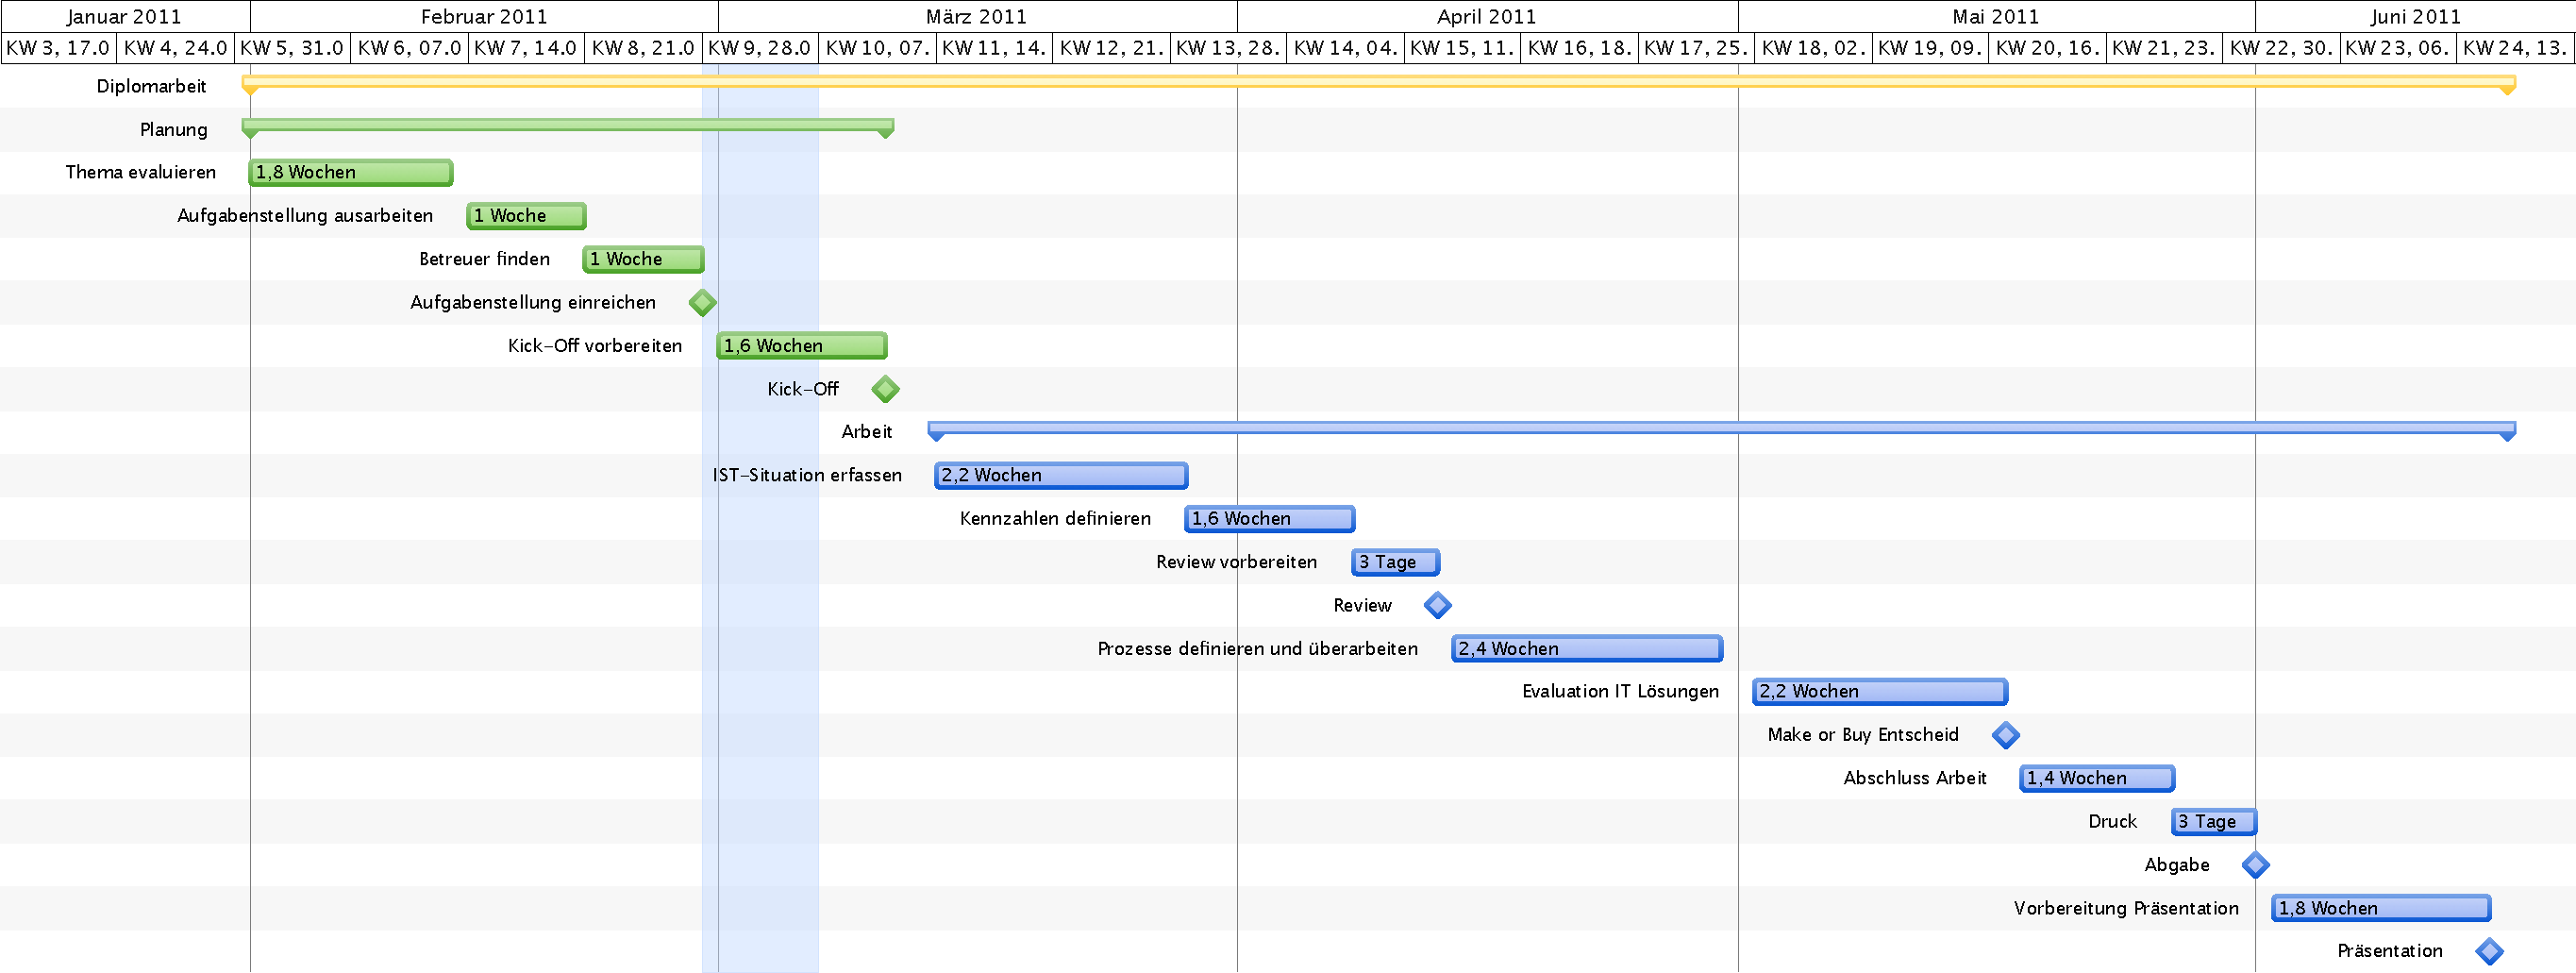
\includegraphics[width=1\textwidth,angle=0]{./bilder/anhang/projektplanung.pdf}
\caption{Projektplan der Diplomarbeit aus Merlin}
\label{pic:projektplan}
\end{center}
\end{figure}

Ich bin mir bewusst, dass es eine eher optimistische Projektplanung ist. Jedoch
steht mir, aus administrativen Gründen der HSZ-T, nur noch dieser Zeitraum für
die Durchführung der Diplomarbeit übrig um mein Studium erfolgreich abschliessen
zu können. Trotz der optimistischen Planung bin ich zuversichtlich, diese
im gegebenen Zeitrahmen umsetzen und abschliessen zu können.

\section{Termine}
In der Tablle \ref{tab:termine_diplomarbeit} sind alle Termine, die sich aus 
dem Projektplan, den bekannten Terminen und Wunschterminen ergeben, in chronologischer
Reihenfolge ihrer Durchführung aufgelistet.

Zusätzlich habe ich sie mit den abhängenden Arbeitspaketen
und Resultaten ergänzt, die zum Zeitpunkt des Termins vorhanden und erfüllt
sein sollten.

\begin{table}[htbp]
\begin{center}
    \begin{tabular}{llll}
        \toprule & & \multicolumn{2}{c}{\textbf{Abhängende}} \\
        \textbf{Datum} & \textbf{Termin} & \textbf{Arbeitspakete} & \textbf{Resultate} \\
        \midrule 28.02.2011 & Aufgabenstellung einreichen & P1, P2, P3 & - \\
        \midrule 11.03.2011 & Kick-Off Meeting & P4 & -\\
        \midrule 13.04.2011 & Review Termin & P5, P6, P7 & R1, R2, R3 \\
        \midrule 17.05.2011 & ``Make or Buy''-Entscheid & P8, P9 & R4, R5, R6 \\
        \midrule 01.06.2011 & Abgabe Diplomarbeit & P10, P11 & R7 \\
        \midrule 15.06.2011 & Präsentation Diplomarbeit & P12 & - \\
        \bottomrule
    \end{tabular}
    \caption{Auflistung der Termine der Diplomarbeit}
    \label{tab:termine_diplomarbeit}
\end{center}
\end{table}

\section{Versionsverwaltung}
Zur besseren Nachvollziehbarkeit meiner Diplomarbeit führe ich seit Beginn an
ein Repository mit git\footnote{Freie Software zur Versionsverwaltung von Dateien,
\url{http://git-scm.com/}} und ein ausführliches Arbeitsprotokoll als Wikipage.
Meinen aktuellen Stand inklusive aller Unterlagen veröffentliche ich auf der 
Plattform github\footnote{Hosting Dienst, \url{https://github.com/}}. Diese 
Informationen sind öffentlich verfügbar und für jedermann unter folgenden 
Adressen zugänglich:

\subsection{git Repository}
\url{https://github.com/sspross/diplomarbeit}

\subsection{Wiki}
\url{https://github.com/sspross/diplomarbeit/wiki}

\subsection{Arbeitsprotokoll}
\url{https://github.com/sspross/diplomarbeit/wiki/arbeitsprotokoll}

\section{Erreichte Ziele}
In der nachfolgenden Tabelle \ref{tab:erreichte_ziele} sind alle Ziele gemäss 
den erwarteten Resultaten der Aufgabenstellung aufgelistet. Alle 
erwarteten Ziele wurden erreicht.

\begin{table}[htbp]
\begin{center}
    \begin{tabular}{p{10cm}lcl}
        \toprule \textbf{Ziel} & \textbf{Resultat} & \textbf{Stand} \\
        \midrule Die Ist-Situation im Bereich Projektablauf der allink.creative
            ist beschrieben und abgebildet. & R1 & erfüllt \\
        \midrule Eine Übersicht über die bestehende Software bei allink.creative
            wurde erstellt. & R2 & erfüllt \\
        \midrule Die Anforderungen an den neuen Prozess inkl. Kennzahlen, die auf 
            Projektebene gemessen werden sollen, wurden definiert. & R3 
            & erfüllt \\
        \midrule Das Konzept des neuen und überarbeiteten Prozesses ist 
            vorhanden. & R4 & erfüllt \\
        \midrule Eine Übersicht über die bestehende Software bei allink.creative
            in der neuen Prozesslandschaft wurde erstellt. & R5 & erfüllt \\
        \midrule Eine Softwareempfehlung für die komplette Prozessabbildung
            wurde erstellt und begründet. & R6 & erfüllt \\
        \midrule Ein ``Make or Buy''-Entscheid wurde mit dem Auftraggeber 
            getroffen und festgehalten. & R7 & erfüllt \\
        \bottomrule
    \end{tabular}
    \caption{Auflistung der erwarteten Resultate mit Stand der Erfüllung}
    \label{tab:erreichte_ziele}
\end{center}
\end{table}
  
  \chapter{Protokolle}
  \section{Kick-Off Protokoll}
  \section{Design Review Protokoll}
  \section{Arbeitsprotokoll}
  
  \listoffigures
  \listoftables
  % \lstlistoflistings
  
  \bibliographystyle{unsrtnat}
  \bibliography{literaturverzeichnis}

\end{document}